% =========================================================
% main.tex - Academic Thesis Template (Optimized)
% =========================================================
\documentclass[12pt,a4paper,oneside]{report}

% -------------------- Page layout --------------------
\usepackage[
    a4paper,
    left=3.0cm,
    right=2.5cm,
    top=2.5cm,
    bottom=2.5cm,
    headheight=15pt % Tránh cảnh báo của fancyhdr nếu dùng sau này
]{geometry}

% -------------------- Encoding and language --------------------
\usepackage[utf8]{inputenc}
\usepackage[T1]{fontenc}
\usepackage[english]{babel}
\usepackage{algorithm}
\usepackage{algpseudocode}
\usepackage{url}
\usepackage{listings}
% -------------------- Font and Micro-typography --------------------
% Sử dụng New Times Roman chuẩn học thuật cho cả text và math
\usepackage{newtxtext}
\usepackage{newtxmath} % Đã bao gồm toán tập hợp, KHÔNG dùng chung với amssymb

% Microtype: Bí quyết giúp văn bản upscale, tự động sửa lỗi tràn lề, giãn chữ cực đẹp
\usepackage{microtype} 

\usepackage{setspace}
\onehalfspacing % Giãn dòng 1.5 chuẩn luận văn

% -------------------- Paragraph formatting --------------------
\usepackage{indentfirst} % Lùi đầu dòng ở cả đoạn đầu tiên sau tiêu đề
\setlength{\parindent}{1.25cm}
\setlength{\parskip}{0pt}

% -------------------- Figures & Graphics --------------------
\usepackage{graphicx}
\usepackage{float}
\usepackage{subcaption}
\graphicspath{{figures/}{images/}{outputs/figures/}}

% -------------------- Tables --------------------
\usepackage{booktabs}
\usepackage{array}
\usepackage{multirow}
\usepackage{makecell}
\usepackage{tabularx}
\usepackage{adjustbox}
\usepackage[table]{xcolor}
\usepackage{ragged2e}


% Cấu hình siunitx chuẩn phiên bản mới v3
\usepackage{siunitx}
\sisetup{
    round-mode = places,
    round-precision = 2,
    detect-all
}

% Định nghĩa lại cột X của tabularx để tự động xuống dòng và căn trái đẹp mắt
\newcolumntype{Y}{>{\RaggedRight\arraybackslash}X}
\newcommand{\tablefont}{\footnotesize} % Font chữ nhỏ gọn cho bảng data lớn

% -------------------- Diagrams (TikZ) --------------------
\usepackage{tikz}
\usetikzlibrary{arrows.meta, positioning, shapes.geometric, fit}

% Safe inline code cho tên file hoặc biến máy tính
\newcommand{\code}[1]{\texttt{\detokenize{#1}}}

% -------------------- Captions --------------------
\usepackage{caption}
\captionsetup{
    font=small,
    labelfont=bf,
    labelsep=colon,
    format=plain,
    justification=justified,
    singlelinecheck=true % Nếu caption chỉ có 1 dòng -> tự động căn giữa
}

% -------------------- Math --------------------
\usepackage{amsmath}
% \usepackage{amssymb} % ĐÃ KHÓA: Tránh xung đột với newtxmath
\usepackage{tabularray}
\usepackage{seqsplit} % Thư viện chuyên dụng để bẻ đôi các chuỗi ký tự siêu dài
% -------------------- Lists --------------------
\usepackage{enumitem}
\setlist{nosep} % Tối ưu khoảng cách các item trong list, không bị hở quá rộng

% -------------------- References and links --------------------
\usepackage[hidelinks]{hyperref}
\usepackage[nameinlink,noabbrev]{cleveref} % Cần đặt sau hyperref
% -------------------- Bibliography --------------------
\usepackage{csquotes} % Thêm dòng này để sửa lỗi
\usepackage[
    backend=biber,
    style=ieee,         % Kiểu IEEE (1, 2, 3), đổi thành style=apa nếu thuộc khối kinh tế/xã hội
    sorting=none
]{biblatex}
\addbibresource{references.bib}

% Không dùng \sloppy vì làm giãn chữ rất xấu. Microtype phía trên đã giải quyết việc này.
\emergencystretch=0.5em 

% =========================================================
% DOCUMENT BODY
% =========================================================
\begin{document}

% -------------------- Front matter --------------------
\pagenumbering{roman} % Đánh số trang kiểu i, ii, iii cho phần mở đầu

% =========================================================
% File: frontmatter/frontmatter.tex
% =========================================================

\pagenumbering{arabic}

% Nhập các cấu phần giao diện chính
% =========================================================
% File: frontmatter/cover.tex
% =========================================================

% ---------------------------------------------------------
% TRANG 1: OUTSIDE COVER (TRANG BÌA CHÍNH CÓ LOGO)
% ---------------------------------------------------------
\begin{titlepage}
    \centering
    \singlespacing
    
    % Tên trường đại học & Viện
    {\large \MakeUppercase{The University of Danang} \par}
    {\large \textbf{\MakeUppercase{VNUK Institute for Research and Executive Education}} \par}
    
    \vspace{1.5cm}
    
    % Khu vực chèn Logo trường (bỏ comment '%' nếu bạn đã có file ảnh logo)
    
\includegraphics[width=0.3\textwidth]{figures/vn-uk-logo.png} 
    
    \vspace{2.0cm}
    
    % Tên đề tài Luận văn (Viết hoa, Chữ đậm, Cỡ lớn)
    {\Large \bfseries \MakeUppercase{%
        Vision-Based Running Technique Classification from In-the-Wild Internet Videos using Markerless Pose Estimation and Deep Learning
        \vspace{0.2cm}%
    } \par}

    
    \vspace{0.5cm}
    
    % Tác giả
    {\large \textit{by} \par}
    \vspace{0.2cm}
    {\large \bfseries \MakeUppercase{Tran Cong Quoc Huy} \par}
    
    \vspace{1cm}
    
    % Giảng viên hướng dẫn
    {\large \textit{under the supervision of} \par}
    \vspace{0.2cm}
    {\large \bfseries NGUYEN CHI THIEN \par}
    \vspace{0.1cm}
    {\small VNUK Institute for Research and Executive Education, The University of Da Nang \par}
    
    \vfill
    
    % Địa điểm, thời gian dưới đáy trang
    {\large \textbf{Da Nang}, May 2026 \par}
\end{titlepage}


% ---------------------------------------------------------
% TRANG 2: INSIDE TITLE PAGE (TRANG BÌA LÓT CÓ CHỮ KÝ)
% ---------------------------------------------------------
\begin{titlepage}
    \centering
    \singlespacing
    
    % Thay thế toàn bộ cụm tiêu đề cũ bằng cụm này:
    {\Large \bfseries \MakeUppercase{%
        Vision-Based Running Technique Classification from In-the-Wild Internet Videos using Markerless Pose Estimation and Deep Learning
        \vspace{0.2cm}%
    } \par}

    
    \vspace{0.5cm} % Khoảng cách chuyển giao xuống phần thông tin tiếp theo
        
    % Tác giả
    {\large \textit{by} \par}
    \vspace{0.2cm}
    {\large \bfseries Tran Cong Quoc Huy \par}
    
    \vspace{0.5cm} % Khoảng cách chuyển giao xuống phần thông tin tiếp theo
    
    % Phần text nộp bài chuẩn quy định
    {\small Submitted to the Department of Computer Science and Engineering (CSE), \\
    VNUK Institute of Research and Executive Education, The University of Da Nang \\
    in Partial Fulfillment of the Requirements for the Degree of \\
    \textbf{Bachelor in Computer Science and Engineering} \par}
    
    \vspace{1.0cm}
    {\large Da Nang, 6/2026 \par}
    
    \vspace{2.5cm}
    
    % Khu vực ký tên (Căn lề chuẩn theo biểu mẫu mẫu)
    \flushleft
    \setlength{\tabcolsep}{0pt}
    \begin{tabular}{p{0.4\textwidth}r}
        Signature of Author: & \makebox[5cm]{\hrulefill} \\
        & Tran Cong Quoc Huy, \\
        & Student ID: 22040005 \\
        [2cm]
        Certified by: & \makebox[5cm]{\hrulefill} \\
        & \textbf{Nguyen Chi Thien} \\
        & Thesis Supervisor \\
        [2cm]
        Accepted by: & \makebox[5cm]{\hrulefill} \\
        & \textbf{[Full Name of Head of Department]} \\
        & Head of Department \\
    \end{tabular}
\end{titlepage}
\clearpage

% =========================================================
% File: frontmatter/declaration.tex
% =========================================================
\chapter*{Declaration}
\addcontentsline{toc}{chapter}{Declaration}

I hereby declare that the work presented in this thesis, titled ``Vision-Based Running Technique Classification from In-the-Wild Internet Videos using Markerless Pose Estimation and Deep Learning'', is entirely my own original research conducted under the supervision of Nguyen Chi Thien. 

All primary and secondary data sources, software tools, literature review materials, and code repositories utilized during this investigation have been appropriately cited and acknowledged in compliance with standard academic protocols. No part of this work has been previously submitted, in whole or in part, for any other degree or qualification at VNUK or any other educational institution.

\vspace{2.0cm}

\noindent
\begin{tabularx}{\textwidth}{@{} Y X @{}}
    \textbf{Date:} 10/06/2026 & \multicolumn{1}{c}{\textbf{Candidate's Signature}} \\[1.5cm]
    & \multicolumn{1}{c}{Tran Cong Quoc Huy}
\end{tabularx}
\clearpage

% =========================================================
% File: frontmatter/acknowledgement.tex
% =========================================================
\chapter*{Acknowledgements}
\addcontentsline{toc}{chapter}{Acknowledgements}

I would like to express my deepest gratitude to my supervisor, Nguyen Chi Thien, for his invaluable guidance, continuous academic support, and constructive feedback throughout the development of this research project. His expertise in machine learning and computer vision has been instrumental in shaping the methodology and analysis of this work.

I extend my appreciation to the faculty members of the Computer Science and Engineering (CSE) department at VNUK for providing a rigorous and stimulating research environment, as well as the necessary computational infrastructure that made this study possible.

Finally, I am profoundly grateful to my peers and my family for their enduring patience, encouragement, and understanding during the writing of this thesis.
\clearpage

% =========================================================
% File: frontmatter/abstract.tex
% =========================================================
\chapter*{Abstract}
\addcontentsline{toc}{chapter}{Abstract}

This study addresses the problem of vision-based running technique classification utilizing unconstrained, in-the-wild internet videos. Traditional biomechanical analysis relies heavily on marker-based motion capture, which is restricted to controlled laboratory settings. To bridge this research gap, we propose an automated computer vision pipeline that processes raw internet running videos using markerless pose estimation via MediaPipe. The structural framework extracts a custom spatial-temporal signal \code{contact_diff} through sequential landmark filtering and normalization. An autocorrelation-based automatic gait cycle detection system is established to isolate distinct strides, which are subsequently downsampled into a standardized 8-frame gait phase representation.

The classification task evaluates and compares landmark-based classifiers alongside an image-based MobileNetV2 + LSTM pipeline. To diagnose performance bottlenecks, comprehensive model, signal, and feature ablation studies are performed against a handmade cycle segmentation upper bound and an automatic baseline. While the system demonstrates that markerless pose sequences can effectively encode distinct running-technique characteristics when cycles are isolated cleanly, comprehensive error analysis reveals significant performance degradation in fully automated end-to-end extraction. Specifically, the handmade upper-bound pipeline achieves a test macro-F1 of 0.8991 and an accuracy of 0.9107 on the controlled test split, whereas the fully automatic autocorrelation-based baseline reaches a macro-F1 of 0.5417 and an accuracy of 0.5455. A further 5-fold video-level cross-validation robustness check confirms the same trend under a shared MLP protocol: handmade cycles achieve 0.860 $\pm$ 0.016 macro-F1, while autocorr cycles achieve 0.615 $\pm$ 0.081, leaving a fair gap of 0.245 macro-F1. A 100-permutation test on the autocorr MLP setting does not reach statistical significance ($p = 0.2475$), suggesting that the autocorr-derived features remain noisy and are not yet robustly separable under a simple classifier. The dataset contains 75 videos and 152 extracted running cycles, but the upper-bound and automatic baseline metrics are reported on their respective controlled test splits rather than on the full dataset. The empirical findings indicate that future deployment readiness depends fundamentally on improving upstream cycle-boundary precision rather than classifier architectural complexity.

\vspace{1.0cm}
\noindent \textbf{Keywords:} Markerless Pose Estimation, Action Classification, Gait Cycle Detection, Deep Learning, Biomechanics.

\clearpage


\tableofcontents
\clearpage
\listoffigures
\clearpage
\listoftables

\clearpage

% -------------------- Chapters --------------------
\pagenumbering{arabic} % Reset và chuyển sang đánh số trang kiểu 1, 2, 3 cho nội dung chính

% =====================================================================
% chapters/01_introduction.tex
% Chapter 1 — Introduction
% Project: Vision-Based Running Technique Classification from In-the-Wild
%          Internet Videos using Markerless Pose Estimation and Deep Learning
%
% No empirical metrics appear here. References use citation keys from the
% thesis bibliography.
% =====================================================================

\chapter{Introduction}
\label{ch:introduction}

% ---------------------------------------------------------------------
\section{Background}
\label{sec:intro-background}

Running technique --- the manner in which a person coordinates posture, foot
strike, stride, and limb motion through the running cycle --- has a direct
bearing on athletic performance, training efficiency, and the risk of
overuse injury \cite{novacheck1998biomechanics}. Coaches, clinicians, and runners
therefore have a long-standing interest in assessing whether a given running
form is sound or in need of correction. Distinguishing "correct" from "false"
technique is, however, a subtle judgement: the diagnostic information is
distributed across the whole kinematic chain and is expressed only as the body
moves periodically through repeated running cycles, rather than in any single
static posture \cite{inostroza2025runningcycle, cutting1978gaitperiodicity}.

Traditional approaches to running analysis are accurate but costly to apply at
scale. Optical marker-based motion capture provides laboratory-grade kinematics
but requires controlled environments, calibrated multi-camera rigs, and marker
placement; wearable inertial sensors enable field measurement but require
body-worn instrumentation and calibration; and expert visual inspection depends
on scarce specialist time and is inherently subjective
\cite{panconi2024markerless, bulling2014tutorial}. None of these
modalities can be applied retrospectively to footage that was not captured with
them in mind.

At the same time, \emph{in-the-wild} running videos --- clips recorded with
ordinary cameras and shared on the internet --- are abundant. This footage is an
enormous, untapped source of running data, but it is also noisy and
uncontrolled: it varies in camera viewpoint, resolution, frame rate, lighting,
and framing, and it carries no instrumentation or ground-truth measurement
\cite{topham2023hpesurvey}. Recent advances in \emph{markerless pose estimation}
make it possible to recover body landmarks directly from such ordinary RGB
video, with per-landmark confidence values, and thereby open the possibility of
analysing running technique from video that was never intended for biomechanical
study \cite{topham2023hpesurvey, lugaresi2019mediapipe, bazarevsky2020blazepose}. This thesis
investigates whether, and under what conditions, that possibility can be realised
with deep learning.

% ---------------------------------------------------------------------
\section{Problem Statement}
\label{sec:intro-problem}

The problem addressed in this thesis is stated as follows: \emph{given an
in-the-wild running video, classify the running technique as correct or false
using markerless pose estimation and deep learning.} The input is an ordinary
single-runner video with no instrumentation or calibration; the desired output
is a binary technique label, ideally accompanied by an indication of confidence.
The task must be solved without the controlled conditions assumed by
marker-based or sensor-based methods, relying instead on landmarks recovered
from the raw footage.

Solving this problem in the wild raises a set of inter-related challenges:

\begin{itemize}
  \item \textbf{Camera viewpoint variation.} Clips are filmed from arbitrary and
        inconsistent angles, so the same technique appears differently across
        videos.
  \item \textbf{Uncontrolled resolution and frame rate.} Spatial resolution and
        temporal sampling (FPS) differ between clips, affecting both pose
        quality and the temporal granularity of the running cycle.
  \item \textbf{Pose-landmark noise.} Markerless estimates from uncontrolled
        footage are noisier and less certain than laboratory measurements.
  \item \textbf{Missing or unstable lower-body landmarks.} The ankle, heel, and
        toe landmarks most diagnostic of running form are also the most
        frequently occluded, blurred, or mislocalised.
  \item \textbf{Foot-strike and cycle-boundary ambiguity.} The events that
        define a running cycle are themselves hard to localise reliably from
        noisy signals.
  \item \textbf{Automatic cycle detection affects classification.} Because the
        classifier operates on segmented cycles, errors in automatic cycle
        detection propagate into the final decision, coupling the two stages.
\end{itemize}

These challenges motivate a design that separates the difficulty of
\emph{classification} from the difficulty of automatic \emph{cycle detection},
so that the contribution of each can be measured rather than conflated.

% ---------------------------------------------------------------------
\section{Research Questions}
\label{sec:intro-rqs}

The thesis is organised around seven research questions:

\begin{description}
  \item[RQ1.] Can pose-based classifiers distinguish correct from false running
        technique when running cycles are manually or otherwise reliably
        segmented?
  \item[RQ2.] How much classification performance is lost when handmade cycles
        are replaced by automatic autocorrelation-based cycle detection?
  \item[RQ3.] Which motion signal is most reliable for automatic running-cycle
        detection?
  \item[RQ4.] Which model architecture is most suitable for classifying
        eight-phase pose sequences?
  \item[RQ5.] How do the feature representation and the number of frames sampled
        per cycle affect classification performance?
  \item[RQ6.] How does an image-based representation compare with a
        landmark-based representation under the same automatic
        (autocorrelation) pipeline?
  \item[RQ7.] How do cycle-level aggregation, decision-threshold selection, and
        pose/cycle quality affect the interpretation of the final results?
\end{description}

RQ1 establishes whether the task is solvable in principle; RQ2 quantifies the
cost of automation; RQ3--RQ5 examine the design choices internal to the
automatic pipeline; RQ6 addresses the representation question; and RQ7 concerns
how results should be measured and interpreted.

% ---------------------------------------------------------------------
\section{Contributions}
\label{sec:intro-contributions}

In addressing these questions, the thesis makes the following contributions:

\begin{enumerate}
  \item A complete markerless, pose-based pipeline for classifying running
        technique from in-the-wild internet videos, spanning pose estimation,
        landmark filtering and normalisation, motion-signal extraction,
        running-cycle detection, phase sampling, representation, deep-learning
        classification, and evaluation.
  \item A matched experimental design comprising a \emph{handmade upper bound},
        which characterises classification given reliable segmentation, and an
        \emph{autocorrelation-based automatic baseline}, which uses only
        information available from the video itself; the pairing isolates the
        effect of automatic cycle detection.
  \item An \emph{eight-phase} running-cycle representation that normalises for
        cadence so that cycles of differing duration become directly comparable.
  \item A set of controlled ablation studies on model architecture, detection
        signal, feature representation, and frames per cycle.
  \item Extended analyses comparing landmark-based and image-based
        representations on an identical cycle source, comparing cycle-level and
        video-level evaluation, examining decision-threshold selection, and
        relating pose and cycle quality to classification accuracy.
  \item A disciplined separation between \emph{historical development} results
        --- retained as method-evolution evidence --- and \emph{controlled
        benchmark} results obtained under a single fixed, leakage-free protocol,
        ensuring that development-stage milestones are not mistaken for
        benchmarks.
\end{enumerate}

% ---------------------------------------------------------------------
\section{Thesis Structure}
\label{sec:intro-structure}

The remainder of the thesis is organised as follows.
Chapter~\ref{ch:literature-review} reviews the relevant literature on running
technique, motion-analysis modalities, markerless pose estimation, running-cycle
detection, pose- and image-based classification, and evaluation protocols, and
identifies the research gap.
Chapter~\ref{ch:methodology} describes the proposed framework in detail,
including the dataset and leakage-free splitting protocol, pose estimation,
landmark filtering and normalisation, motion-signal extraction, the three
cycle-detection methods, eight-phase sampling, the landmark and image
representations, the classification models, the cycle- and video-level
prediction scheme, and threshold selection.
Chapter~\ref{ch:experimental-setup} specifies the experimental setup, including
training configurations, evaluation metrics, and the reporting protocol that
separates controlled from historical results.
Chapter~\ref{ch:results} reports the empirical results: dataset statistics, the
handmade upper bound, the automatic baseline, the ablation studies, the
historical version history, and the extended analyses.
Chapter~\ref{ch:discussion} interprets these results, locating where performance
is gained and lost across the pipeline.
Chapter~\ref{ch:conclusion} summarises the findings, restates the answers to the
research questions, and outlines directions for future work. Throughout, the
scope of the conclusions is kept commensurate with the dataset and protocol
used, and no claim of real-world deployment readiness is made.

% End of Chapter 1
% =====================================================================
% chapters/02_literature_review.tex
% Chapter 2 — Literature Review
% Project: Vision-Based Running Technique Classification from In-the-Wild
%          Internet Videos using Markerless Pose Estimation and Deep Learning
%
% Required preamble packages (declare in main.tex):
%   \usepackage{booktabs}  \usepackage{array}  \usepackage{tabularx}
%
% Citation keys are drawn from references.bib and from the verified papers in
% the project literature folder. No empirical results appear here.
% =====================================================================

\chapter{Literature Review}
\label{ch:literature-review}

This chapter reviews the research relevant to vision-based running-technique
classification. It proceeds from the biomechanics of running form, through the
sensing modalities used to measure it, to the pose-estimation, cycle-detection,
and classification methods on which an automatic pipeline can be built. It then
examines how multi-cycle video data should be evaluated, and closes by stating
the research gap that this thesis addresses.

% ---------------------------------------------------------------------
\section{Running Technique Analysis}
\label{sec:lit-running}

Running technique, or running form, is commonly characterised by a small set of
inter-related kinematic descriptors: the manner of \emph{foot strike} (rearfoot,
midfoot, or forefoot contact), trunk and pelvis \emph{posture}, \emph{stride}
parameters such as step length and cadence, and the \emph{coordination} of the
upper and lower limbs through the gait cycle
\cite{novacheck1998biomechanics, inostroza2025runningcycle}. These
descriptors are not independent; for example, an over-strided rearfoot contact
typically coincides with a more extended knee at touchdown and altered trunk
lean, so that "correct" and "incorrect" technique are better understood as
configurations of the whole kinematic chain than as single isolated events
\cite{dicharry2010kinematics}.

A recurring theme in the running-biomechanics literature is that technique is
expressed \emph{periodically}: the discriminative information lives in how the
body moves through repeated running cycles rather than in any single static
frame \cite{inostroza2025runningcycle, cutting1978gaitperiodicity}. This has two
consequences for an automatic system. First, the unit of analysis should be a
running cycle, not an arbitrary frame window. Second, the descriptors most
diagnostic of form --- foot contact, knee and ankle behaviour at touchdown, limb
swing --- are concentrated in the lower body, which motivates particular
attention to lower-limb measurement (Section~\ref{sec:lit-pose}).

% ---------------------------------------------------------------------
\section{Marker-Based and Markerless Motion Analysis}
\label{sec:lit-modalities}

Three broad modalities are used to capture running kinematics:
optical \emph{marker-based} motion capture, \emph{wearable} inertial sensors,
and \emph{markerless} video-based pose estimation. Marker-based systems track
reflective markers with calibrated multi-camera rigs and are widely regarded as
the laboratory reference for kinematic accuracy, but they require controlled
environments, specialist hardware, and marker placement, which makes them
unsuitable for analysing the large volumes of uncontrolled footage found online
\cite{panconi2024markerless}. Wearable inertial measurement units estimate
segment motion from accelerometers and gyroscopes; they are portable and usable
outdoors, but require body-worn instrumentation, calibration, and drift
correction, and are likewise absent from existing internet video
\cite{fiaz2026gaitphase, bulling2014tutorial}.

Markerless video-based analysis estimates body configuration directly from
ordinary RGB video using learned pose-estimation models. It requires no
instrumentation and can in principle be applied to any recording, which is what
makes it the only viable modality for \emph{in-the-wild} internet video. The
trade-off is reduced and less certain measurement: estimates are noisier,
subject to occlusion and viewpoint variation, and accompanied only by
model-internal confidence rather than physical calibration
\cite{lugaresi2019mediapipe, bazarevsky2020blazepose, topham2023hpesurvey}.
Table~\ref{tab:modalities} summarises the comparison that motivates the
markerless choice in this thesis.

\begin{table}[htbp]
\centering
\caption{Comparison of motion-analysis modalities for running-technique
measurement.}
\label{tab:modalities}
\renewcommand{\arraystretch}{1.2}
\begin{tabularx}{\textwidth}{l X X X}
\toprule
Property & Marker-based & Wearable sensors & Markerless video \\
\midrule
Instrumentation & Markers $+$ multi-camera rig & Body-worn IMUs & None (RGB video only) \\
Environment & Controlled lab & Field-capable & Any, incl.\ in-the-wild \\
Kinematic accuracy & Reference standard & High, drift-prone & Lower, noisier \\
Setup / calibration & High & Moderate & None \\
Applicable to internet video & No & No & Yes \\
Uncertainty signal & Physical calibration & Sensor model & Per-landmark confidence \\
\bottomrule
\end{tabularx}
\end{table}

The implication is direct: only markerless video can be applied retrospectively
to uncontrolled internet footage, so an in-the-wild system must accept the
attendant measurement noise and design around it rather than assume
laboratory-grade input.

% ---------------------------------------------------------------------
\section{Human Pose Estimation for Movement Understanding}
\label{sec:lit-pose}

Modern markerless pipelines rely on human pose estimators that localise a fixed
set of anatomical \emph{landmarks} (joints) per frame. For single-person,
monocular video, lightweight estimators produce \emph{2D landmarks} --- image
coordinates for each joint --- typically accompanied by a \emph{visibility} or
\emph{confidence} value that reflects the model's certainty that the joint is
present and correctly located
\cite{cao2019openpose, lugaresi2019mediapipe, bazarevsky2020blazepose}. This
per-landmark confidence is central to any downstream use: it allows low-quality
detections to be filtered or down-weighted, and it provides a measurable proxy
for input quality that can later be related to classification performance.

For running-technique analysis the \emph{lower-body} landmarks --- hips, knees,
ankles, heels, and toes --- are the most informative, because foot strike, knee
behaviour at touchdown, and ankle motion are precisely the descriptors that
distinguish good from poor form (Section~\ref{sec:lit-running})
\cite{novacheck1998biomechanics}. Unfortunately, these same landmarks are also
the least \emph{stable}. The feet and ankles are small, fast-moving, frequently
occluded by the opposite leg or by motion blur, and often near the image
boundary; their estimated positions therefore carry more noise and lower
confidence than torso landmarks
\cite{topham2023hpesurvey, panconi2024markerless}. This tension --- the most
diagnostic joints being the least reliably estimated --- is a defining challenge
of markerless running analysis and recurs throughout this thesis, both in the
choice of motion signals (Section~\ref{sec:lit-cycle}) and in the analysis of
error sources.

% ---------------------------------------------------------------------
\section{Running Cycle and Gait Phase Detection}
\label{sec:lit-cycle}

Because running is periodic, a natural pre-processing step is to segment the
continuous pose sequence into individual running cycles, conventionally bounded
by successive \emph{foot-strike} events of the same foot
(foot-strike-to-foot-strike) \cite{inostroza2025runningcycle, ghoussayni2004gait}.
Reliable cycle boundaries are a prerequisite for any phase-aligned
representation: if cycles are mis-bounded, samples drawn from "the same phase"
across different cycles will in fact correspond to different moments of the gait,
undermining comparison.

Two families of method are used to find these boundaries. \emph{Event-based}
methods detect foot-strike directly from a chosen motion signal, for instance by
locating peaks or valleys in a vertical-displacement or foot-contact proxy
signal \cite{ghoussayni2004gait, zhang2025heelstrike}. \emph{Periodicity-based}
methods first estimate the dominant period of the motion --- classically via
\emph{autocorrelation} of a one-dimensional signal --- and then use that period
to constrain or validate candidate boundaries, which makes detection more robust
to isolated spurious peaks \cite{cutting1978gaitperiodicity}. A practical
pipeline often combines the two: an autocorrelation estimate provides the
expected cycle length, and peak/valley detection on a foot-contact signal
supplies the actual boundaries, with the period acting as a consistency check.

The choice of signal interacts strongly with stability
(Section~\ref{sec:lit-pose}). Signals derived from torso or hip vertical motion
are smooth and easy to detect but only indirectly related to foot strike, while
signals derived from the noisy foot and heel landmarks are more directly tied to
contact events but more prone to error \cite{zhang2025heelstrike}. Selecting a
signal is therefore a trade-off between detection coverage and boundary
precision, a trade-off this thesis examines explicitly.

% ---------------------------------------------------------------------
\section{Pose-Based Action Classification}
\label{sec:lit-pose-class}

Once cycles are segmented and sampled, the resulting landmark sequences can be
classified by a range of neural architectures, ordered roughly by how much
temporal structure they model \cite{yan2018stgcn, jangua2021gait2dposes}. A
\emph{multilayer perceptron} (MLP) treats the flattened sequence as a
fixed-length vector and learns a static mapping; it is fast and low-variance but
ignores temporal ordering, which can be adequate when inputs are short and
well-aligned. A \emph{one-dimensional convolutional neural network} (1D-CNN)
applies temporal convolutions across the sequence, capturing local motion
patterns with relatively few parameters \cite{ordonez2016deephar}.

Recurrent models capture longer-range temporal dependencies. A
\emph{bidirectional long short-term memory} network (BiLSTM) processes the
sequence in both directions, allowing each phase to be interpreted in the
context of the whole cycle \cite{hochreiter1997lstm, schuster1997bidirectional}.
A \emph{CNN-BiLSTM} hybrid first extracts local features with convolutions and
then models their temporal evolution with a BiLSTM, combining local pattern
extraction with sequence modelling \cite{donahue2015lrcn}. More expressive
recurrent and hybrid models can represent richer dynamics, but on small or noisy
datasets their additional capacity also increases the risk of overfitting --- a
consideration that is especially relevant when the input cycles are themselves
imperfectly segmented.

% ---------------------------------------------------------------------
\section{Image-Based Video Classification}
\label{sec:lit-image}

An alternative to landmark sequences is to classify the \emph{appearance} of the
runner directly. Here each sampled phase is represented as an RGB crop centred
on the runner, and a convolutional backbone extracts visual features that a
temporal model then aggregates over the cycle. A widely used efficient design
pairs a lightweight pretrained convolutional backbone such as
\emph{MobileNetV2} with a recurrent temporal head such as an LSTM
(a MobileNetV2--LSTM model): the backbone encodes each frame into a feature
vector, and the LSTM models the sequence of per-frame features to produce a
cycle-level prediction \cite{sandler2018mobilenetv2, donahue2015lrcn}.

The appeal of image-based representations is that RGB crops retain information
absent from sparse landmarks --- body silhouette, limb contour, clothing-relative
motion, and surrounding visual context --- which could in principle aid
classification \cite{topham2023hpesurvey}. The cost is a substantially larger and
higher-variance input. Image pipelines must learn to ignore appearance variation
(background, clothing, lighting) that landmarks discard by construction, which
typically demands more training data; they are also sensitive to the stability
of the runner-centred crop, which itself depends on the same noisy pose estimates
discussed in Section~\ref{sec:lit-pose}.
Table~\ref{tab:representations} contrasts the two representation families.

\begin{table}[htbp]
\centering
\caption{Comparison of landmark-based and image-based cycle representations.}
\label{tab:representations}
\renewcommand{\arraystretch}{1.2}
\begin{tabularx}{\textwidth}{l X X}
\toprule
Property & Landmark-based & Image-based (RGB crop) \\
\midrule
Input per phase & Joint coordinates ($+$ confidence) & RGB crop (e.g.\ $224\times224$) \\
Dimensionality & Low & High \\
Information retained & Joint geometry only & Silhouette, contour, context \\
Invariance & Appearance-invariant by design & Must be learned \\
Typical model & MLP / CNN / BiLSTM / CNN-BiLSTM & CNN backbone $+$ temporal head \\
Data requirement & Lower & Higher \\
Main vulnerability & Pose-estimation noise & Crop instability, overfitting \\
\bottomrule
\end{tabularx}
\end{table}

% ---------------------------------------------------------------------
\section{Evaluation Protocols for Multi-Cycle Video Data}
\label{sec:lit-eval}

A subtlety specific to cycle-based video analysis is the choice of evaluation
unit. Because one video can yield several cycles, predictions may be scored at
the \emph{cycle level} --- treating each detected cycle as an independent sample
--- or at the \emph{video level} --- aggregating a video's cycles into a single
prediction by, for example, majority vote, mean probability, or
confidence-weighted vote \cite{singh2018gaitsurvey}. The two views answer
different questions: cycle-level metrics characterise per-cycle discriminability,
whereas video-level metrics estimate the performance a user would experience,
since the practical unit of interest is the video.

Two methodological hazards accompany this choice. First, if cycles from the same
video are allowed to appear in both training and test sets, the evaluation leaks
video-specific information and inflates scores; splitting strictly \emph{by
video} is therefore essential. Second, comparisons across
pipelines are only fair when the evaluation unit and protocol are held fixed; a
model evaluated on whole-video sequences is not directly comparable to one
evaluated per cycle. Sound practice is to report the split protocol explicitly,
to fix the evaluation unit within any comparison, and to state whether a tuned
decision threshold was used and how it was selected.

% ---------------------------------------------------------------------
\section{Research Gap}
\label{sec:lit-gap}

The reviewed literature establishes that running technique is a periodic,
lower-body-dominated phenomenon (Section~\ref{sec:lit-running}); that only
markerless video can be applied to in-the-wild footage, at the price of noisy
estimates (Section~\ref{sec:lit-modalities}); that the most diagnostic landmarks
are also the least stable (Section~\ref{sec:lit-pose}); and that cycle detection,
representation, and classification each offer well-studied options
(Sections~\ref{sec:lit-cycle}--\ref{sec:lit-image}). What remains
under-addressed is their combination on \emph{uncontrolled internet video} under
a rigorous, leakage-free evaluation.

Specifically, three gaps motivate this thesis. First, prior work seldom
\emph{separates} the contribution of automatic cycle detection from that of the
classifier; without a controlled upper bound, it is unclear whether failures
stem from segmentation or from learning. Second, landmark-based and image-based
representations are rarely compared on an \emph{identical} automatic cycle source
under a fixed split, so apparent representation advantages may merely reflect
protocol differences --- and historical, differently-evaluated milestones risk
being mistaken for controlled benchmarks. Third, the interaction between
pose/cycle quality and classification accuracy on in-the-wild data is rarely
quantified, leaving the dominant error source unidentified. This thesis addresses
these gaps with a matched handmade-upper-bound versus automatic-baseline design,
a controlled landmark-versus-image comparison on a shared cycle source, and an
explicit analysis of cycle-level versus video-level evaluation, threshold
selection, and pose/cycle quality
(Chapters~\ref{ch:methodology}--\ref{ch:discussion}).

% End of Chapter 2
% =====================================================================
% chapters/03_methodology.tex
% Chapter 3 — Methodology
% Project: Vision-Based Running Technique Classification from In-the-Wild
%          Internet Videos using Markerless Pose Estimation and Deep Learning
%
% Required preamble packages (declare in main.tex):
%   \usepackage{booktabs}  \usepackage{array}  \usepackage{tabularx}
%   \usepackage{graphicx}  \usepackage{amsmath}
%   \usepackage{algorithm}  \usepackage{algpseudocode}
%
% This chapter describes methods only. No empirical results appear here.
% Citation keys are drawn from references.bib and the verified project
% literature papers. Method/contribution sentences carry no citation.
% =====================================================================

\chapter{Methodology}
\label{ch:methodology}

This chapter describes the proposed framework for classifying running technique
from in-the-wild video. It follows the pipeline end to end: pose estimation,
landmark filtering and normalisation, motion-signal extraction, cycle detection,
eight-phase sampling, the two cycle representations, the classification models,
the cycle- and video-level prediction scheme, and threshold selection. No
results are reported; the experimental outcomes appear in
Chapter~\ref{ch:results}.

% ---------------------------------------------------------------------
\section{Overview of the Proposed Framework}
\label{sec:method-overview}

The framework transforms a raw video into a correct/false technique prediction
through the stages shown in Figure~\ref{fig:method_pipeline}: markerless pose
estimation, landmark filtering, motion-signal extraction, running-cycle
detection, eight-phase sampling, construction of a pose-based or image-based
representation, deep-learning classification, and evaluation. A deliberate
design principle is to keep the cycle-detection stage interchangeable so that a
manual (handmade) segmentation, a rule-based autocorrelation detector, and a
learned boundary detector can be compared under an otherwise identical pipeline,
isolating the effect of cycle source on performance.

\begin{figure}[htbp]
\centering
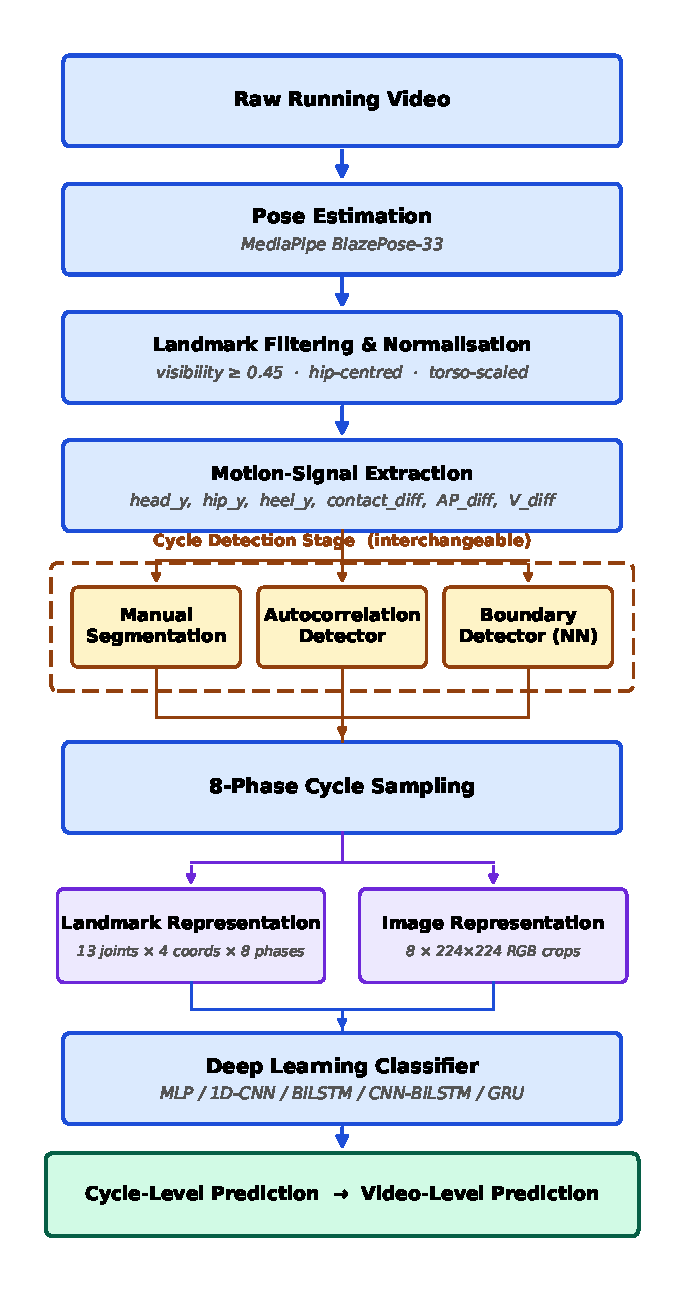
\includegraphics[width=\textwidth,height=0.75\textheight,keepaspectratio]{figures_new/fig31_pipeline}
\caption{Overall framework for vision-based running technique classification
from in-the-wild videos. Starting from a raw running video, the pipeline
applies markerless pose estimation, filters and normalises the resulting
landmarks, extracts one-dimensional motion signals, and detects running cycles
via one of three interchangeable detectors (manual, autocorrelation-based, or
learned boundary detector). Each accepted cycle is resampled into eight phases
and encoded as either a landmark sequence or a set of image crops, which are
then classified by a deep-learning model. Cycle-level predictions are
aggregated into a final video-level decision.}
\label{fig:method_pipeline}
\end{figure}


% ---------------------------------------------------------------------
\section{Dataset Construction and Splitting Protocol}
\label{sec:method-dataset}

The dataset consists of single-runner clips labelled as correct or false
technique. Because a single video yields multiple running cycles, the
\emph{splitting protocol} is critical: the data are split \emph{by video
identifier}, so that all cycles extracted from a given video are confined to a
single partition (train, validation, or test). This prevents \emph{leakage} of
video-specific information --- if cycles from one video appeared in both training
and test sets, the model could recognise the video rather than the technique,
inflating the apparent accuracy. The split is fixed once
and reused unchanged across every experiment so that all pipelines are evaluated
on the same videos. The resulting per-split counts are reported in
Chapter~\ref{ch:results}.

% ---------------------------------------------------------------------
\section{Markerless Pose Estimation}
\label{sec:method-pose}

Each frame is processed by a markerless pose estimator that returns a fixed set
of body landmarks with image coordinates and a per-landmark \emph{visibility}
(confidence) value \cite{lugaresi2019mediapipe, bazarevsky2020blazepose}. The
visibility value is retained throughout the pipeline: it is used both to filter
unreliable detections (Section~\ref{sec:method-filter}) and, in later analysis,
as a measurable proxy for input quality. A reduced set of \emph{selected
landmarks} relevant to running technique --- nose, shoulders, hips, knees,
ankles, heels, and foot indices --- is used as the basis of the pose
representation, since the discriminative information for running form is
concentrated in the trunk orientation and the lower limbs
(Chapter~\ref{ch:literature-review}). The lower-limb landmarks (ankles, heels,
toes) are the most diagnostic but also the most prone to noise and occlusion,
which motivates the filtering and normalisation described next.
Figure~\ref{fig:pose_estimation} shows an example of the estimator output on a
running frame.

\begin{figure}[htbp]
\centering
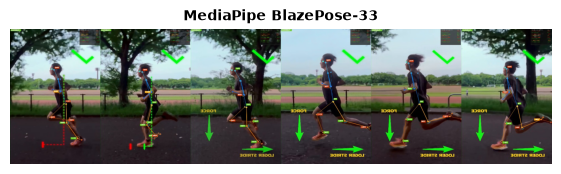
\includegraphics[width=0.60\textwidth]{figures_new/fig33_pose_estimation}
\caption{MediaPipe BlazePose-33 applied to a sample running frame. The model
produces 33 body landmarks with per-landmark visibility scores. A subset of
13 landmarks relevant to running form --- nose, hips, knees, ankles, heels,
and foot indices --- is selected for all downstream processing.}
\label{fig:pose_estimation}
\end{figure}

% ---------------------------------------------------------------------
\section{Landmark Filtering and Normalization}
\label{sec:method-filter}

Raw landmark trajectories are filtered before use. Detections whose visibility
falls below a threshold are treated as unreliable and discarded or interpolated,
and the resulting per-joint trajectories are temporally smoothed to suppress
high-frequency jitter introduced by frame-to-frame estimation noise.
Visibility-based screening is applied with particular care to the nose and heel
landmarks, which serve as quality indicators for the head and foot regions
respectively.

Landmarks are then \emph{normalised} so that the representation is invariant to
the runner's position and apparent scale in the frame. Coordinates are expressed
relative to a body-centred reference and scaled by a body-size measure (for
example a torso-span normalisation), removing dependence on where the runner
appears in the image and how far they are from the camera. This normalisation is
essential for in-the-wild video, where framing, zoom, and runner position vary
arbitrarily between clips. Figure~\ref{fig:landmark_normalization} illustrates
the effect on the vertical trajectories of the nose, hip, and heel landmarks.

\begin{figure}[htbp]
\centering
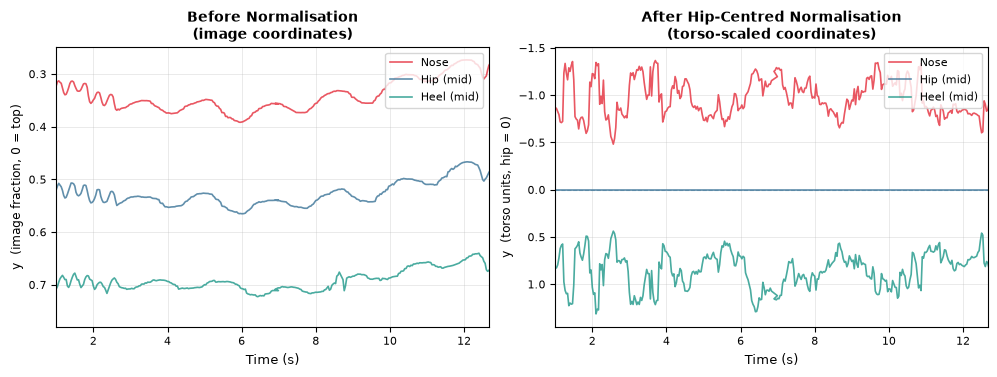
\includegraphics[width=\textwidth]{figures_new/fig34_landmark_normalization}
\caption{Landmark vertical coordinates before (left) and after (right)
hip-centred normalisation for an example video. Before normalisation, the
trajectories drift with the runner's absolute position in the frame. After
normalisation, all trajectories oscillate stably about zero (the hip
reference) with consistent amplitude regardless of camera distance or
runner position.}
\label{fig:landmark_normalization}
\end{figure}

% ---------------------------------------------------------------------
\section{Motion Signal Extraction}
\label{sec:method-signals}

From the filtered, normalised landmarks, a set of one-dimensional \emph{motion
signals} is derived for cycle detection. Each signal is a scalar time series
whose periodic structure reflects the running cycle.
Table~\ref{tab:signals} lists the candidate signals.

\begin{table}[htbp]
\centering
\caption{Candidate one-dimensional motion signals used for running-cycle
detection.}
\label{tab:signals}
\renewcommand{\arraystretch}{1.2}
\begin{tabularx}{\textwidth}{l X}
\toprule
Signal & Definition (per frame) \\
\midrule
head-Y & Vertical position of the head/nose landmark \\
hip-Y & Vertical position of the hip (pelvis) landmark \\
heel-Y & Vertical position of the heel landmark \\
toe-Y & Vertical position of the toe (foot index) landmark \\
\texttt{contact\_diff} & Foot-contact proxy from the heel/toe landmarks (left--right contact difference) \\
\texttt{AP\_diff} & Anterior--posterior (horizontal) displacement difference between feet \\
\texttt{V\_diff} & Vertical displacement difference between feet \\
\bottomrule
\end{tabularx}
\end{table}

The vertical-oscillation signals (head-Y, hip-Y) are smooth and easy to detect
but only indirectly related to foot strike, whereas the foot-derived signals
(\texttt{contact\_diff}, \texttt{AP\_diff}, \texttt{V\_diff}, heel-Y, toe-Y) are
more directly tied to ground contact but noisier
(Chapter~\ref{ch:literature-review}). The pipeline supports any single signal as
the detection driver; the comparison of signals is treated as an ablation
(Chapter~\ref{ch:results}). Each signal is smoothed and detrended before
detection to stabilise period estimation. Figure~\ref{fig:motion_signals} shows
the four main signals over an example running clip.

\begin{figure}[htbp]
\centering
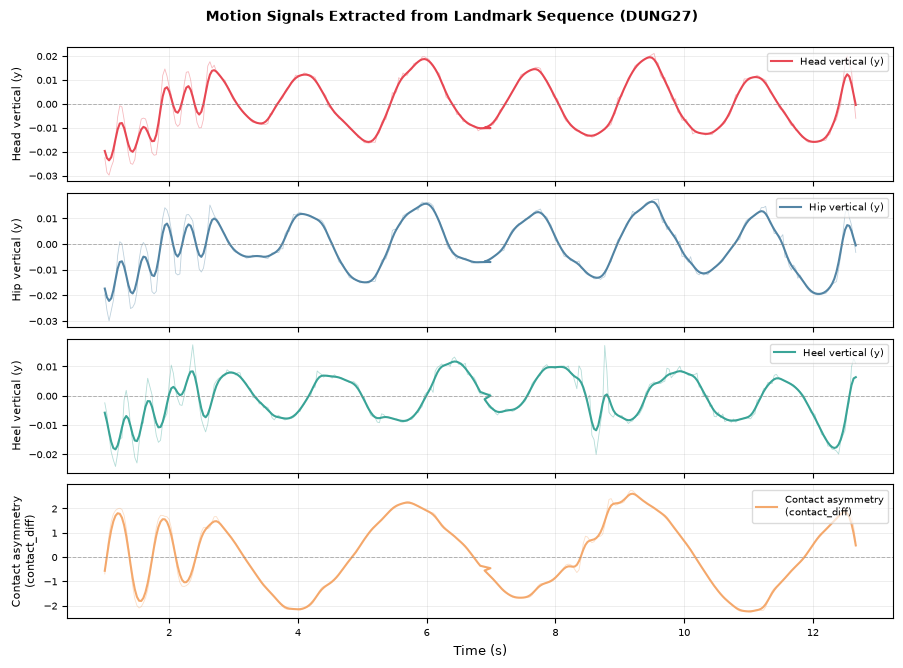
\includegraphics[width=\textwidth]{figures_new/fig35_motion_signals}
\caption{Motion signals extracted from a single running video (DUNG27). Faint
lines show the raw detrended signal; solid lines show the Gaussian-smoothed
version ($\sigma=2$). The periodic oscillation visible in all four signals
reflects the running cycle; \texttt{contact\_diff} captures left--right
foot-contact asymmetry and is used as the primary cycle-detection driver.}
\label{fig:motion_signals}
\end{figure}

% ---------------------------------------------------------------------
\section{Running Cycle Detection}
\label{sec:method-cycle}

A running cycle is bounded by successive foot-strike events of the same foot
(foot-strike-to-foot-strike, FS-to-FS). The framework provides three
interchangeable detectors --- a manual handmade segmentation, an automatic
autocorrelation-based detector, and a learned boundary detector --- followed by a
common quality-filtering step.

\subsection{Handmade Cycle Segmentation}
\label{sec:method-handmade}

In the handmade pipeline, cycle boundaries are determined manually so that each
extracted cycle is correctly segmented. This pipeline is used as an
\emph{upper bound}: it characterises how well the representation and classifier
can separate correct from false technique \emph{when segmentation is reliable},
and thereby separates the difficulty of classification from the difficulty of
automatic detection. It is not a deployable baseline, since a fielded system
cannot rely on manual segmentation.

\subsection{Autocorrelation-Based Automatic Cycle Detection}
\label{sec:method-autocorr}

The automatic baseline detects cycles without manual input. A chosen motion
signal is smoothed and detrended; its dominant period is estimated by
\emph{autocorrelation}; candidate foot-strike boundaries are located by
peak/valley detection on the signal; and the estimated period is used to
validate boundary spacing, including a correction for spurious double-stride
detections (a two-stride fix). Candidate cycles are then passed to quality
filtering. Algorithm~\ref{alg:autocorr_cycle_detection} summarises the procedure.

\begin{algorithm}[htbp]
\caption{Autocorrelation-based running cycle detection}
\label{alg:autocorr_cycle_detection}
\begin{algorithmic}[1]
\Require Filtered landmark sequence, motion signal $s$, duration bounds $[\tau_{\min}, \tau_{\max}]$
\Ensure Set of accepted FS-to-FS running cycles $C$
\State $x \gets \textsc{ExtractSignal}(s)$
\State $x \gets \textsc{Smooth}(x)$
\State $\hat{p} \gets \textsc{EstimatePeriod}(\textsc{Autocorrelation}(x))$
\State $P \gets \textsc{FindCandidateBoundaries}(x)$
\State $P \gets \textsc{TwoStrideFix}(P, \hat{p})$
\State $C \gets \emptyset$
\For{each consecutive boundary pair $(f_i, f_{i+1})$ in $P$}
    \State $\tau \gets \textsc{Duration}(f_i, f_{i+1})$
    \If{$\tau_{\min} \leq \tau \leq \tau_{\max}$ and visibility is adequate}
        \State $C \gets C \cup \{(f_i, f_{i+1})\}$
    \EndIf
\EndFor
\State \Return $\textsc{QualityFilter}(C)$
\end{algorithmic}
\end{algorithm}

This detector is the main \emph{automatic baseline} of the thesis: it uses only
information available from the video itself, with no fixed-margin assumption on
boundary placement, and produces cycles directly comparable to the handmade
ones because the downstream stages are identical.
Figure~\ref{fig:cycle_boundaries} shows an example detection result.

\begin{figure}[htbp]
\centering
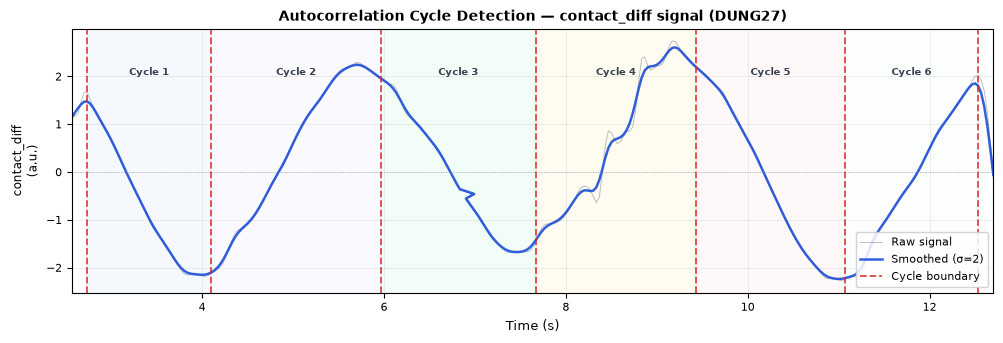
\includegraphics[width=\textwidth]{figures_new/fig36_cycle_boundaries}
\caption{Running cycle boundaries detected by the autocorrelation-based
detector overlaid on the \texttt{contact\_diff} signal for an example video
(DUNG27). Alternating shaded bands correspond to individual FS-to-FS cycles;
red dashed lines mark the detected boundaries. The periodic structure of the
signal makes the boundaries reliably locatable by the autocorrelation
procedure.}
\label{fig:cycle_boundaries}
\end{figure}

\subsection{Boundary Detector-Based Cycle Detection}
\label{sec:method-bd}

As a learned alternative to rule-based detection, a \emph{boundary detector}
(BD) replaces autocorrelation with a trained sequence model
\cite{zhang2025heelstrike, sui2020gaitsegmentation}. The BD is a BiLSTM that
consumes a sliding window of frames and predicts the probability that the
central frame is a foot-strike boundary; ground-truth boundaries are taken from
the endpoints of handmade single-cycle clips. At inference, the per-frame
boundary probabilities are smoothed and thresholded, peaks are taken as
boundaries, and consecutive boundaries define FS-to-FS cycles, which are then
quality-filtered exactly as for the autocorrelation detector. The BD is treated
as a supplementary pipeline.

\subsection{Cycle Quality Filtering}
\label{sec:method-quality}

Regardless of detector, candidate cycles pass through a common
\emph{quality-filtering} step before being accepted. Cycles whose duration falls
outside the plausible running-cycle range, whose constituent landmarks have
insufficient visibility, or which cannot be sampled into the required number of
phases are rejected. This step enforces a consistent definition of a usable
cycle across all pipelines, so that the only intended difference between them is
how boundaries are obtained. The rejected-cycle statistics are later used to
analyse where the automatic pipeline loses data (Chapter~\ref{ch:results}).

% ---------------------------------------------------------------------
\section{Eight-Phase Cycle Sampling}
\label{sec:method-phases}

Each accepted cycle is resampled into a fixed number of \emph{gait phases} so
that cycles of different absolute durations become directly comparable. Eight
phases are used, spanning one full FS-to-FS cycle:

\begin{figure}[htbp]
    \centering
    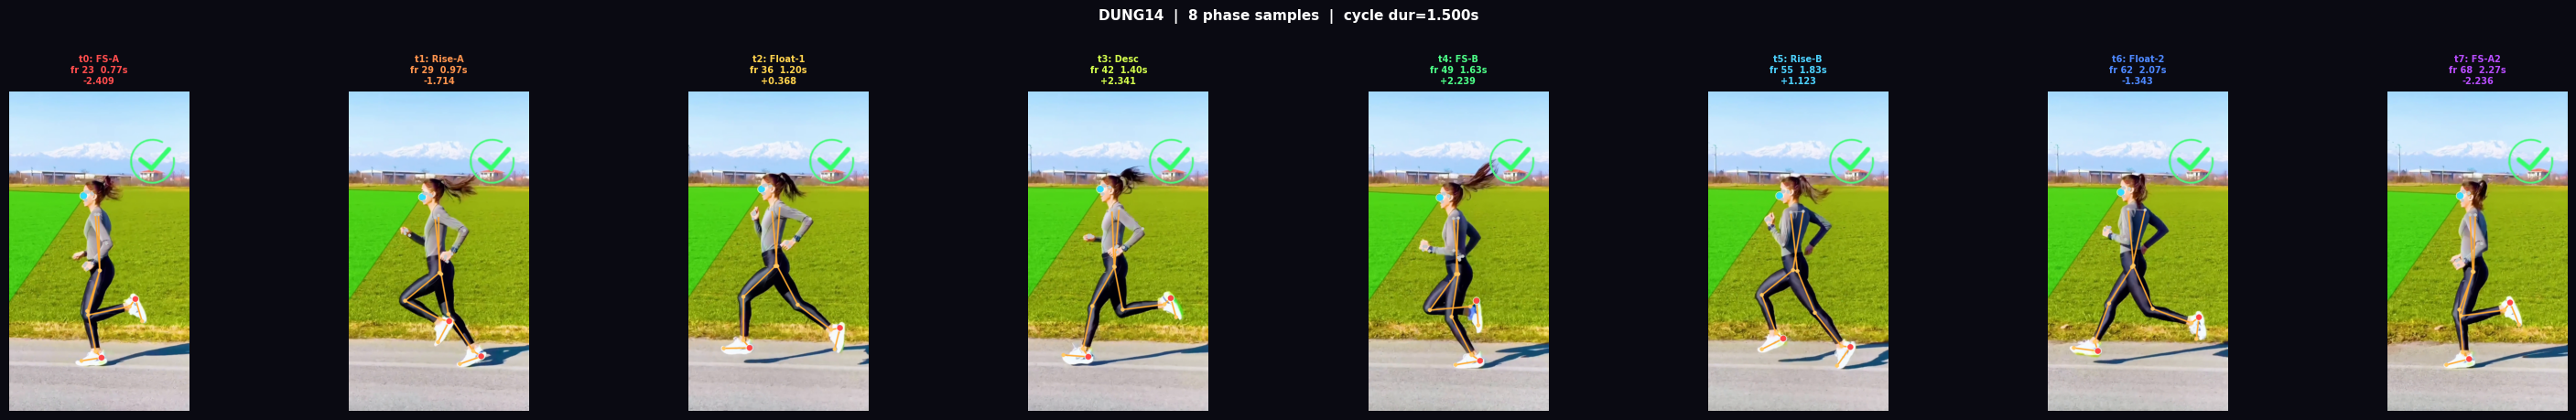
\includegraphics[width=\textwidth]{figures/8_sample_phase.png}
    \caption{Example of eight-phase sampling from an automatically detected running cycle.}
    \label{fig:8phase_sampling}
\end{figure}

Sampling at fixed phases (rather than fixed frame offsets) normalises for
cadence, so that "the same phase" denotes the same point in the running cycle
across runners and speeds \cite{inostroza2025runningcycle}. The eight-phase
sampling defines the temporal length of every representation that follows; its
sufficiency relative to finer samplings is examined as a frames-per-cycle
ablation in Chapter~\ref{ch:results}.

% ---------------------------------------------------------------------
\section{Landmark-Based Pose Representation}
\label{sec:method-landmark-rep}

In the landmark representation, each of the eight phases is encoded by the
normalised coordinates of the selected landmarks, optionally augmented with
\emph{velocity} (the inter-phase change in coordinates) and other derived
quantities. The result is a compact, fixed-size sequence per cycle that is
invariant to appearance by construction. This representation is the basis of the
main automatic baseline and of the model, feature, and signal ablations.

% ---------------------------------------------------------------------
\section{Image-Based Cycle Representation}
\label{sec:method-image-rep}

In the image representation, each phase is encoded as an RGB \emph{crop} centred
on the runner. A stable bounding box is computed per cycle from the pose
estimates (for example a median box over the cycle) and used to crop and resize
each sampled frame to a fixed resolution, yielding an eight-frame image sequence
per cycle. This representation retains appearance information absent from
landmarks --- silhouette, limb contour, clothing-relative motion --- at the cost
of higher dimensionality and sensitivity to crop stability. To ensure a
\emph{fair} comparison, the image pipeline uses exactly the same automatic cycle
source as the landmark baseline, so that the two differ only in representation
(Chapter~\ref{ch:results}).

% ---------------------------------------------------------------------
\section{Classification Models}
\label{sec:method-models}

Several classifiers are used across the representations and pipelines, chosen to
span a range of temporal modelling capacity.
Figure~\ref{fig:model_architectures} shows the layer-by-layer architectures of
the four landmark-based models.

\begin{figure}[htbp]
\centering
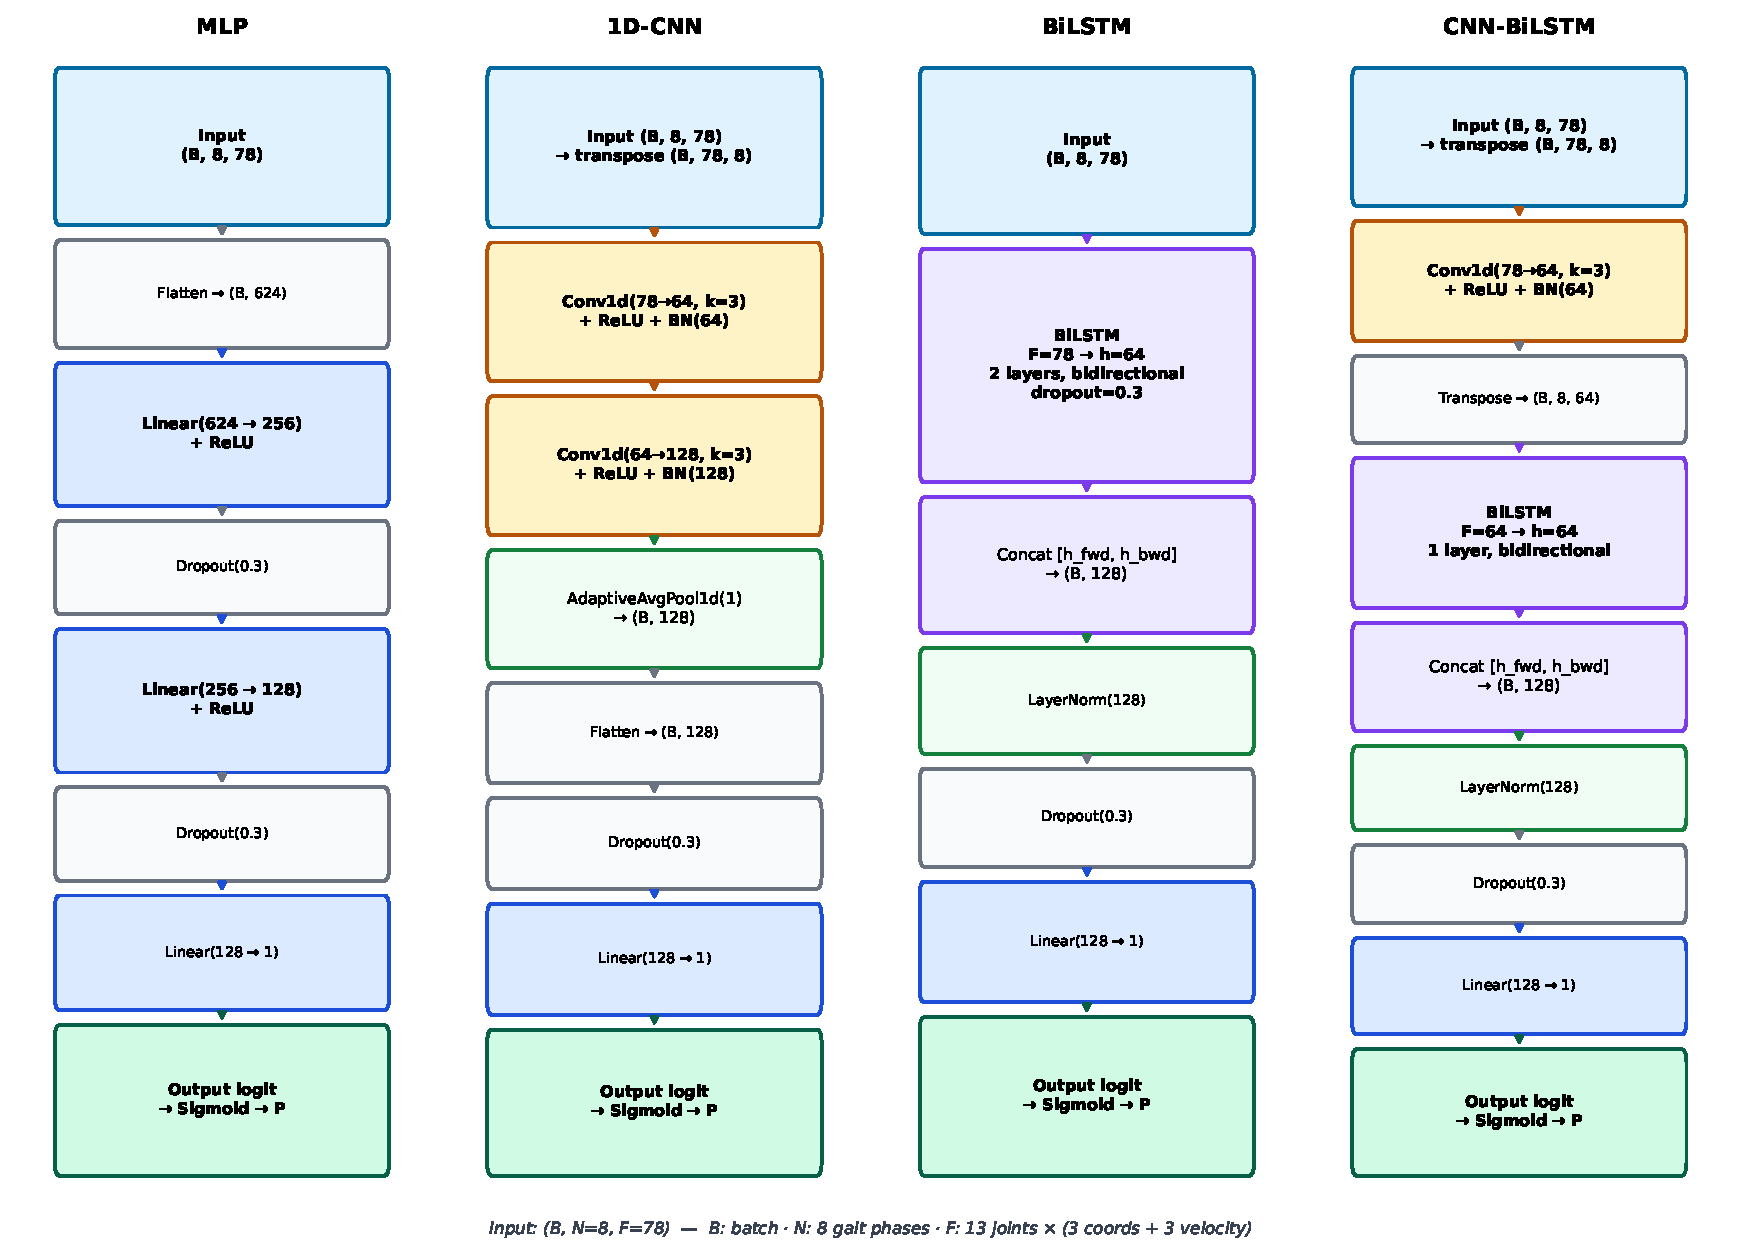
\includegraphics[width=\textwidth]{figures_new/fig_model_architectures}
\caption{Layer-by-layer architectures of the four landmark-based classifiers.
All models receive an input tensor of shape $(B,\,8,\,78)$ --- batch size,
eight gait phases, and $F{=}78$ features (13 joints $\times$ 3 coordinates
$+$ 3 velocity components) --- and produce a single binary logit. Colour
indicates layer type: blue --- linear; amber --- convolutional; violet ---
recurrent (BiLSTM); green --- normalisation or pooling; grey --- utility
(flatten, dropout).}
\label{fig:model_architectures}
\end{figure}

\subsection{MLP Baseline}
\label{sec:method-mlp}

The multilayer perceptron flattens the eight-phase landmark sequence into a
single vector and learns a static mapping to the correct/false decision. It does
not model temporal order, but is fast and low-variance, which can be
advantageous for short, well-aligned inputs.

\subsection{One-Dimensional CNN}
\label{sec:method-cnn}

The 1D-CNN applies temporal convolutions across the eight-phase sequence,
capturing local kinematic patterns with relatively few parameters before a
classification head \cite{ordonez2016deephar}.

\subsection{BiLSTM}
\label{sec:method-bilstm}

The bidirectional LSTM processes the phase sequence in both directions, so that
each phase is represented in the context of the entire cycle, capturing
longer-range temporal dependencies than the convolutional model
\cite{hochreiter1997lstm, schuster1997bidirectional}.

\subsection{CNN-BiLSTM}
\label{sec:method-cnn-bilstm}

The CNN-BiLSTM hybrid first extracts local features with one-dimensional
convolutions and then models their temporal evolution with a BiLSTM, combining
local pattern extraction with sequence modelling \cite{donahue2015lrcn}.

\subsection{MobileNetV2-LSTM}
\label{sec:method-mobilenet}

For the image representation, a MobileNetV2--LSTM model is used: a MobileNetV2
convolutional backbone encodes each RGB crop into a feature vector, and an LSTM
aggregates the eight per-phase feature vectors into a cycle-level prediction. The
backbone may be frozen or partially fine-tuned
\cite{sandler2018mobilenetv2, donahue2015lrcn}. This model operates on image
crops rather than landmark coordinates and is therefore used only in the
image-based pipeline.

\subsection{GRU for Raw Sequence Modeling}
\label{sec:method-gru}

To probe whether explicit cycle cutting is necessary, a recurrent model
(a gated recurrent unit, GRU, alongside a BiLSTM) is applied to the
\emph{raw} pose sequence of an entire video, without segmentation into cycles.
Here one sample corresponds to one video, so this is an exploratory,
supplementary configuration rather than part of the cycle-based comparison.

% ---------------------------------------------------------------------
\section{Cycle-Level and Video-Level Prediction}
\label{sec:method-cycle-video}

Because each video yields several cycles, predictions are produced at two
levels. \emph{Cycle-level} prediction treats each detected cycle as an
independent sample. \emph{Video-level} prediction aggregates a video's cycle
predictions into a single decision; three aggregation rules are considered:
\emph{majority vote}, \emph{mean probability}, and \emph{confidence-weighted
vote}. Since the underlying data unit is the video, video-level prediction is
the more faithful measure of practical performance; both levels are reported so
that the effect of aggregation can be examined (Chapter~\ref{ch:results}).

% ---------------------------------------------------------------------
\section{Threshold Selection}
\label{sec:method-threshold}

Each probabilistic classifier requires a \emph{decision threshold} to convert
predicted probabilities into a correct/false label. Two settings are
considered: the default threshold of $0.5$, and a \emph{tuned} threshold
selected on the \emph{validation} set by sweeping candidate thresholds and
choosing the one that maximises validation macro-F1, which is then applied
unchanged to the test set. Selecting the threshold on validation rather than on
test avoids optimistic bias; reporting both the default and the tuned result
makes any threshold overfitting visible. Every reported metric states which
threshold setting it uses.

% ---------------------------------------------------------------------
\section{Implementation Outputs}
\label{sec:method-outputs}

The pipeline is implemented as a sequence of self-contained, configurable
notebooks, each writing standardised outputs --- per-cycle and per-video
prediction files, result summaries, cycle-detection statistics, and diagnostic
figures --- to a fixed directory structure. These artefacts provide the inputs
to the controlled comparisons, ablations, and quality analyses presented in
Chapter~\ref{ch:results}, and are designed so that missing files degrade
gracefully rather than invalidating downstream aggregation.

% End of Chapter 3
% =====================================================================
% chapters/04_experimental_setup.tex
% Chapter 4 — Experimental Setup
% Project: Vision-Based Running Technique Classification from In-the-Wild
%          Internet Videos using Markerless Pose Estimation and Deep Learning
%
% Required preamble packages (declare in main.tex):
%   \usepackage{booktabs}  \usepackage{array}  \usepackage{tabularx}
%   \usepackage{amsmath}
%
% This chapter specifies the experimental protocol only. No empirical results
% appear here; they are reported in Chapter 5. Training hyper-parameters are
% reported only when supported by experiment evidence rather than guessed.
% Architecture parameter counts are configuration facts and are stated where known.
% =====================================================================

\chapter{Experimental Setup}
\label{ch:experimental-setup}

This chapter specifies how the framework of Chapter~\ref{ch:methodology} is
evaluated: the fixed dataset split and evaluation protocol, the experimental
pipelines and their roles, the model training configuration, the evaluation
metrics, and the design of the ablation and extended analyses. No results are
reported here; all empirical outcomes appear in Chapter~\ref{ch:results}.

% ---------------------------------------------------------------------
\section{Dataset Split and Evaluation Protocol}
\label{sec:setup-split}

All experiments use a single \emph{fixed split by video identifier}. Each video
is assigned to exactly one partition --- train, validation, or test --- and all
running cycles extracted from that video inherit its partition. This guarantees
that no cycle from a test video is ever seen during training, preventing the
model from recognising a specific video rather than the technique and thereby
avoiding the optimistic bias that video-level leakage would introduce
. The split is generated once and reused unchanged by every
pipeline and every ablation, so that all configurations are compared on
identical videos.

The validation partition is used for model selection and for decision-threshold
tuning (Section~\ref{sec:setup-metrics} and
Section~\ref{sec:abl-threshold}); the test partition is held out and used only
for final reporting. The per-split counts at both the video and cycle level are
reported with the results in Section~\ref{sec:dataset-stats}, since they
describe the data on which the controlled benchmarks are computed.

% ---------------------------------------------------------------------
\section{Experimental Pipelines}
\label{sec:setup-pipelines}

Five pipelines are evaluated. They share every stage except cycle source and
representation, which is what allows their differences to be attributed to those
two factors. Table~\ref{tab:pipelines} summarises their design and role.

\begin{table}[htbp]
\centering
\caption{Experimental pipelines, their cycle source, representation, models, and intended role. Only the first two rows constitute the main controlled comparison; the image pipeline is an extended representation comparison and the last two are supplementary.}
\label{tab:pipelines}
\renewcommand{\arraystretch}{1.3}
\footnotesize % Giữ nguyên cỡ chữ nhỏ để bảng gọn gàng

% Cấu hình mới: cột 1 và 2 để 'l' (vì chữ ngắn), các cột còn lại dùng 'X' hoặc định dạng của 'X' để tự động xuống dòng.
\begin{tabularx}{\textwidth}{l l X X X}
\toprule
Pipeline & Cycle source & Representation & Model(s) & Role \\
\midrule
Handmade landmark & Manual segmentation & Landmark $+$ velocity & MLP, 1D-CNN, BiLSTM, CNN-BiLSTM & Upper bound (not deployable) \\
\addlinespace
Autocorr landmark & Autocorr.\ (\texttt{contact\_diff}) & Landmark $+$ velocity & MLP, 1D-CNN, BiLSTM, CNN-BiLSTM & Main automatic baseline \\
\addlinespace
Autocorr image & Autocorr.\ (\texttt{contact\_diff}) & RGB crop & MobileNetV2--LSTM & Representation comparison \\
\addlinespace
Boundary detector & Learned BiLSTM boundaries & Landmark $+$ velocity & BiLSTM, CNN-BiLSTM & Supplementary \\
\addlinespace
Raw sequence & None (whole video) & Full landmark sequence & GRU, BiLSTM & Supplementary / exploratory \\
\bottomrule
\end{tabularx}
\end{table}


% ---------------------------------------------------------------------
\section{Model Training Configuration}
\label{sec:setup-training}

All models are trained on the train partition, selected on the validation
partition, and evaluated once on the test partition. The pose-sequence models
operate on eight-phase landmark inputs of shape $(B,\,8,\,78)$, where
$F{=}78$ features comprise 13 selected joints $\times$ 3 coordinates $+$ 3
velocity components (Section~\ref{sec:method-phases}). The layer-by-layer
architectures of the four landmark classifiers are shown in
Figure~\ref{fig:model_architectures}.

The four landmark-sequence models share a common training schedule confirmed
from the experiment notebooks: \textbf{AdamW} optimiser with learning rate
$10^{-3}$ and weight decay $10^{-4}$; \textbf{OneCycleLR} scheduler with
\texttt{pct\_start}$=0.2$; \textbf{BCEWithLogitsLoss} with a class-ratio
\texttt{pos\_weight}; gradient clipping (max norm $1.0$); and early stopping
with patience $15$. Batch size is $16$, maximum epochs $80$, and random seed
$42$.

The image model uses eight RGB crops per detected cycle and a MobileNetV2--LSTM
architecture \cite{sandler2018mobilenetv2, donahue2015lrcn}.
Table~\ref{tab:model-config} summarises the per-model configuration.
The audited MobileNetV2--LSTM experiment uses learning rate $10^{-3}$, batch
size $8$, $40$ epochs, dropout $0.4$, two recurrent layers, weight decay
$10^{-4}$, and random seed $42$.


\begin{table}[htbp]
\centering
\caption{Model configuration confirmed from the experiment notebooks. Parameter
counts are taken from the exported model-ablation report. The four
landmark-sequence models share a common optimizer/scheduler/loss (see text);
per-model architecture details follow Figure~\ref{fig:model_architectures}.}
\label{tab:model-config}
\renewcommand{\arraystretch}{1.18}
\scriptsize
\begin{tabularx}{\textwidth}{
>{\raggedright\arraybackslash}p{0.16\textwidth}
>{\raggedright\arraybackslash}p{0.18\textwidth}
>{\raggedright\arraybackslash}p{0.22\textwidth}
>{\raggedright\arraybackslash}p{0.10\textwidth}
>{\raggedright\arraybackslash}X}
\toprule
Model & Pipeline use & Input & Params & Architecture notes \\
\midrule
MLP & Handmade \& autocorr landmark & $(B,8,78)$ & $193{,}025$ &
  Flatten $\to$ Linear(624$\to$256)+ReLU $\to$ Dropout(0.3) $\to$
  Linear(256$\to$128)+ReLU $\to$ Dropout(0.3) $\to$ Linear(128$\to$1). \\
\addlinespace
1D-CNN & Handmade \& autocorr landmark & $(B,8,78)$ & $40{,}257$ &
  Conv1d(78$\to$64, $k$=3)+ReLU+BN $\to$ Conv1d(64$\to$128, $k$=3)+ReLU+BN
  $\to$ AdaptiveAvgPool1d(1) $\to$ Dropout(0.3) $\to$ Linear(128$\to$1). \\
\addlinespace
BiLSTM & Handmade \& autocorr landmark & $(B,8,78)$ & $173{,}441$ &
  2-layer bidirectional LSTM ($h$=64) $\to$ concat[$h_\text{fwd}$, $h_\text{bwd}$]
  (128-d) $\to$ LayerNorm(128) $\to$ Dropout(0.3) $\to$ Linear(128$\to$1). \\
\addlinespace
CNN-BiLSTM & Handmade \& autocorr landmark & $(B,8,78)$ & $82{,}113$ &
  Conv1d(78$\to$64, $k$=3)+ReLU+BN $\to$ 1-layer BiLSTM ($h$=64) $\to$
  concat (128-d) $\to$ LayerNorm(128) $\to$ Dropout(0.3) $\to$ Linear(128$\to$1). \\
\addlinespace
MobileNetV2--LSTM & Autocorr image pipeline & 8$\times$RGB $224{\times}224$ & --- &
  MobileNetV2 backbone (frozen or fine-tuned) $\to$ 2-layer LSTM
  ($h$=256, dropout=0.4) $\to$ Linear($\to$1).
  lr=$10^{-3}$; batch=8; epochs=40; seed=42. \\
\addlinespace
GRU / BiLSTM (raw) & Supplementary raw-sequence & Full video landmark seq. & --- &
  Whole-video recurrent model; one sample per video. Treated as supplementary
  evidence; detailed hyper-parameters not audited. \\
\bottomrule
\end{tabularx}
\end{table}

Parameter counts for the four landmark models are taken directly from the
exported model-ablation report and are used as a reference for model complexity.
The MobileNetV2--LSTM and raw-sequence rows are included for completeness;
their parameter counts were not exported. All landmark classifiers were trained
under the shared schedule described above; the MobileNetV2--LSTM and
raw-sequence models follow separate configurations noted in their respective
rows.

% ---------------------------------------------------------------------
\section{Evaluation Metrics}
\label{sec:setup-metrics}

The following metrics are used.
\emph{Accuracy}, \emph{precision}, \emph{recall}, and \emph{F1} follow their standard definitions.
The \emph{macro-averaged F1} (macro-F1) is the unweighted mean of per-class F1 over the two classes (correct, false):
\begin{equation}
\mathrm{macro\text{-}F1} =
\frac{1}{2}\left(\mathrm{F1}_{\text{correct}} + \mathrm{F1}_{\text{false}}\right).
\end{equation}

\emph{ROC-AUC} is the area under the receiver-operating-characteristic curve,
which plots the true-positive rate against the false-positive rate as the
decision threshold varies; it summarises ranking quality independently of any
single threshold, with $0.5$ corresponding to chance \cite{fawcett2006roc}.

\paragraph{Why macro-F1 is the primary metric.}
Because the dataset is class-imbalanced at the video level (more false than
correct videos, Section~\ref{sec:dataset-stats}), accuracy can be misleading: a
classifier that favours the majority class can attain deceptively high accuracy
while failing on the minority class. Macro-F1 weights both classes equally
regardless of their frequency, so a model must perform well on \emph{both}
correct and false technique to score well \cite{sokolova2009metrics}. Macro-F1 is
therefore reported as the primary metric throughout, with accuracy, per-class
F1, and ROC-AUC reported alongside it for completeness. ROC-AUC is particularly
useful for separating ranking quality from threshold choice, which is examined
explicitly in Section~\ref{sec:abl-threshold}.

% ---------------------------------------------------------------------
\section{Ablation Study Design}
\label{sec:setup-ablations}

The ablations and extended analyses each vary one factor while holding the
remainder of the pipeline fixed, so that the measured effect can be attributed
to that factor. Table~\ref{tab:ablations} summarises the design; the
corresponding results appear in Chapter~\ref{ch:results}.

\begin{table}[htbp]
\centering
\caption{Design of the ablation studies and extended analyses. Each study varies
one factor on a fixed pipeline and split.}
\label{tab:ablations}
\renewcommand{\arraystretch}{1.3}
\footnotesize
\begin{tabularx}{\textwidth}{l X l X}
\toprule
Study & Varied factor & Pipeline & Held fixed \\
\midrule
Model ablation & Classifier (MLP / 1D-CNN / BiLSTM / CNN-BiLSTM) & Handmade \& Autocorr & Data, split, representation, threshold \\
Feature ablation & Feature set (selected, full-33, $+$velocity, $+$AP/V, $+$contact, $+$all) & Handmade & Model, split, frames \\
Signal ablation & Detection signal (head-Y, hip-Y, heel-Y, toe-Y, \texttt{contact\_diff}, \texttt{AP\_diff}, \texttt{V\_diff}) & Autocorr & Model, split, representation \\
Frames-per-cycle & Frames sampled per cycle (8 / 16 / 24 / 32) & Handmade & Model family, split, representation \\
Representation & Landmark vs.\ image & Autocorr (shared cycle source) & Cycle source, split \\
Cycle vs.\ video & Evaluation unit (cycle vs.\ video aggregation) & Autocorr (and others) & Model, split \\
Threshold & Decision threshold ($0.5$ vs.\ validation-tuned) & All & Model, split \\
Pose/cycle quality & Quality factor (visibility, autocorr., missing-ratio, duration, period) & Autocorr & Model, split \\
Fair-gap robustness & Cycle source under repeated folds and label permutations & Handmade vs.\ autocorr & MLP, video-level CV, threshold $0.5$ \\
\bottomrule
\end{tabularx}
\end{table}

\subsection{Model Ablation}
\label{sec:abl-model}
The four classifiers are compared on identical data for both the handmade and
autocorr pipelines, holding the representation, split, and decision threshold
fixed, to isolate the effect of architecture.

\subsection{Feature Ablation}
\label{sec:abl-feature}
On the handmade pipeline, the input feature set is varied --- from the compact
selected-landmark set through the full landmark set and several
derived-feature augmentations --- with the classifier and all other stages held
fixed, to measure the effect of feature representation.

\subsection{Signal Ablation}
\label{sec:abl-signal}
On the autocorr pipeline, the one-dimensional motion signal driving cycle
detection is varied across the seven candidates of
Table~\ref{tab:signals}, holding the classifier fixed. Both detection
statistics (coverage, period regularity, rejections) and downstream
classification are recorded, since signal choice affects both.

\subsection{Frames-per-Cycle Ablation}
\label{sec:abl-frames}
On the handmade pipeline, the number of frames sampled per cycle is varied
(8/16/24/32) for the sequence models, holding all else fixed, to test whether
temporal resolution beyond eight phases improves classification and at what
computational cost.

\subsection{Representation Ablation}
\label{sec:abl-representation}
The landmark and image representations are compared on the \emph{same}
autocorrelation cycle source and split, so that any difference is attributable
to representation rather than to cycle source or protocol. This analysis is kept
separate from the historical image-based development milestone, which was
recorded under a different protocol and is not a controlled benchmark.

\subsection{Cycle-Level versus Video-Level Evaluation}
\label{sec:abl-cycle-video}
Predictions are evaluated both per cycle and aggregated per video (majority
vote, mean probability, confidence-weighted vote), holding the model and split
fixed, to assess how aggregation affects measured performance. Video-level
results are treated as the more faithful estimate of practical performance.

\subsection{Threshold 0.5 versus Tuned Threshold}
\label{sec:abl-threshold}
For each model, performance at the default $0.5$ threshold is compared with
performance at a threshold selected on the \emph{validation} set (by maximising
validation macro-F1) and applied unchanged to test. Reporting both, together
with the change between them, exposes any threshold overfitting rather than
concealing it.

\subsection{Pose and Cycle Quality Analysis}
\label{sec:abl-quality}
Test cycles from the autocorr pipeline are grouped by pose- and cycle-quality
factors --- landmark visibility, autocorrelation strength, landmark
missing-ratio, cycle duration, and cycle period --- and classification
performance is compared across groups, to locate the dominant source of error in
the automatic pipeline. Because no canonical quality thresholds exist, groups are
formed by a median split, and the resulting group sizes are reported with the
results so that small groups are interpreted cautiously
(Section~\ref{sec:quality}).

\subsection{Fair Gap Robustness Check and Permutation Test}
\label{sec:abl-fair-gap}

The fixed split gives the primary controlled benchmark. Because the validation
and test partitions are small, an additional robustness check is used to test
whether the handmade--autocorr gap is specific to that split. Both cycle sources
are evaluated with the same MLP classifier, 5-fold video-level cross-validation,
the default threshold of $0.5$, and macro-F1 as the main metric. Splitting is
again performed by video identifier, so all cycles from one video remain within
the same fold.

A permutation test is also applied to the autocorr MLP setting. The observed
cross-validation macro-F1 is compared with a null distribution obtained by
randomly permuting the labels and rerunning the same cross-validation procedure.
The test is used as a diagnostic of separability under a simple classifier, not
as a replacement for the controlled benchmark. A non-significant result is
therefore interpreted conservatively: it indicates that the autocorr-derived
features are not robustly separable under that MLP configuration, rather than
proving that no useful signal exists.

% End of Chapter 4

% =====================================================================
% chapters/05_results.tex
% Chapter 5 — Results
% Project: Vision-Based Running Technique Classification from In-the-Wild
%          Internet Videos using Markerless Pose Estimation and Deep Learning
% =====================================================================

\chapter{Results}
\label{ch:results}

This chapter reports the empirical results of the running-technique
classification pipelines. Following the experimental protocol of
Chapter~\ref{ch:experimental-setup}, a strict separation is maintained
between (i)~\emph{controlled benchmark} results, obtained under the fixed
split-by-video protocol with a unified reporting procedure, and
(ii)~\emph{historical development} results, retained only as method-evolution
evidence. All controlled tables use the same fixed train/validation/test
split summarised in Section~\ref{sec:dataset-stats}. A separate fair-gap
robustness check then repeats the handmade--autocorr comparison under
5-fold video-level cross-validation to assess whether the fixed-split gap is
systematic.

% ---------------------------------------------------------------------
\section{Dataset Statistics}
\label{sec:dataset-stats}
% Source file: outputs/dataset/split_summary.csv

The dataset is partitioned by video identifier so that all cycles extracted
from a given video are confined to a single split, preventing video-specific
information from leaking between training and evaluation. Table~\ref{tab:split}
summarises the resulting split.

\begin{table}[htbp]
\centering
\caption[Dataset split by video and by detected running cycle. Source: \protect\path{split_summary.csv}.]{Dataset split by video and by detected running cycle. Source: \path{split_summary.csv}.}
\label{tab:split}
\tablefont
\begin{tabularx}{\textwidth}{X r r r r}
\toprule
\textbf{Split} & \textbf{Videos} & \textbf{Correct videos} & \textbf{False videos} & \textbf{Detected cycles} \\
\midrule
Train       & 52 & 20 & 32 & 97  \\
Validation  & 11 &  5 &  6 & 33  \\
Test        & 12 &  5 &  7 & 22  \\
\midrule
\textbf{Total} & \textbf{75} & \textbf{30} & \textbf{45} & \textbf{152} \\
\bottomrule
\end{tabularx}
\end{table}

The class balance at the video level is moderately skewed
toward the \emph{false} class (45 vs.\ 30), a distribution that motivates the
use of macro-averaged F1 as the primary evaluation metric throughout this
chapter, since macro-F1 weights both classes equally and is therefore
robust to this imbalance \cite{sokolova2009metrics}. The small validation and test
splits (11 and 12 videos respectively) also caution against over-interpreting
single-point differences, a consideration revisited in the discussion of
threshold tuning (Section~\ref{sec:threshold}).

% ---------------------------------------------------------------------
\section{Handmade Landmark Upper Bound}
\label{sec:handmade}
% Source file: outputs/handmade/handmade_results.csv

The handmade landmark pipeline uses manually controlled cycle segmentation and
therefore estimates the upper bound of the landmark representation under clean
cycle boundaries. It is not treated as a deployment baseline. Table~\ref{tab:handmade}
reports the four trained architectures.

\begin{table}[htbp]
\centering
\caption[Handmade landmark upper-bound results. Best macro-F1 and metrics in bold. Source: \protect\path{handmade_results.csv}.]{Handmade landmark upper-bound results. Best macro-F1 and metrics in bold. Source: \path{handmade_results.csv}.}
\label{tab:handmade}
\tablefont
\begin{tabularx}{\textwidth}{X r r r r r}
\toprule
\textbf{Model} & \textbf{Test acc.} & \textbf{Macro-F1} & \textbf{F1-correct} & \textbf{F1-false} & \textbf{ROC-AUC} \\
\midrule
MLP        & 0.8571 & 0.8545 & 0.8293 & 0.8798 & 0.9444 \\
1D-CNN     & 0.8929 & 0.8772 & 0.8889 & 0.8649 & 0.9444 \\
BiLSTM     & 0.8750 & 0.8623 & 0.8889 & 0.8357 & 0.9556 \\
\textbf{CNN-BiLSTM} & \textbf{0.9107} & \textbf{0.8991} & \textbf{0.9333} & \textbf{0.8649} & \textbf{0.9556} \\
\bottomrule
\end{tabularx}
\end{table}

The handmade setting establishes that the landmark representation is
learnable when cycle segmentation is reliable, with all four architectures
exceeding 0.85 macro-F1 and ROC-AUC above 0.94. This directly answers the first research
question: when running cycles are correctly segmented, the markerless pose
representation carries sufficient information for a deep model to discriminate
correct from false technique. The narrow spread across
architectures (macro-F1 0.8545--0.8991) indicates that, given clean cycles,
classification is not strongly architecture-limited.

% ---------------------------------------------------------------------
\section{Autocorr Landmark Baseline}
\label{sec:autocorr-baseline}
% Source files: outputs/autocorr/autocorr_results.csv,
%               outputs/autocorr/autocorr_cycle_stats.csv

The autocorrelation landmark pipeline is the main automatic baseline. It uses
the \texttt{contact\_diff} motion signal, autocorrelation period estimation,
foot-strike-to-foot-strike cycle cutting, no cycle margin, selected landmark
features, and velocity features. Table~\ref{tab:autocorr} reports the
controlled fixed-split results.

\begin{table}[htbp]
\centering
\caption[Autocorr landmark baseline results. Best macro-F1 in bold. Source: \protect\path{autocorr_results.csv}.]{Autocorr landmark baseline results. Best macro-F1 in bold. Source: \path{autocorr_results.csv}.}
\label{tab:autocorr}
\small
\begin{tabular}{lrrrrr}
\toprule
Model & Test acc. & Macro-F1 & F1-correct & F1-false & ROC-AUC \\
\midrule
MLP & 0.5455 & 0.5417 & 0.5000 & 0.5833 & 0.6068 \\
1D-CNN & 0.5000 & 0.3425 & 0.6850 & 0.0000 & 0.5684 \\
BiLSTM & 0.4545 & 0.3714 & 0.7429 & 0.0000 & 0.5342 \\
CNN-BiLSTM & \textbf{0.5909} & \textbf{0.5901} & 0.5333 & 0.6468 & \textbf{0.6370} \\
\bottomrule
\end{tabular}
\end{table}

% SỬA LỖI DÒNG 149 TẠI ĐÂY: Thay \sec:threshold} bằng \ref{sec:threshold}
Although the CNN-BiLSTM has the best fixed-threshold macro-F1 in the raw
autocorr model table, the thesis baseline uses the MLP row in later summary
tables because the threshold analysis in Section~\ref{sec:threshold} shows it
is more stable after validation-based threshold selection. This distinction is
important: the automatic baseline is evaluated not only by its peak
fixed-threshold score but also by its robustness to the complete reporting
protocol. Compared with the handmade upper bound, the autocorr landmark baseline drops
substantially. The best fixed-threshold automatic result reaches only 0.5901
macro-F1, and the robust reported MLP baseline reaches 0.5417 macro-F1. Some
sequential models collapse on the \emph{false} class so dominantly that F1-false reaches 0.0000.
This validation-to-test collapse, combined with ROC-AUC values close to 0.5,
indicates that the limiting factor in the automatic pipeline is not classifier
capacity but the quality and consistency of the automatically segmented
cycles. The contrast with Section~\ref{sec:handmade} is quantified directly in Section~\ref{sec:hm-vs-ac}.

\IfFileExists{figures/autocorr_confusion_matrix.png}{%
\begin{figure}[htbp]
\centering
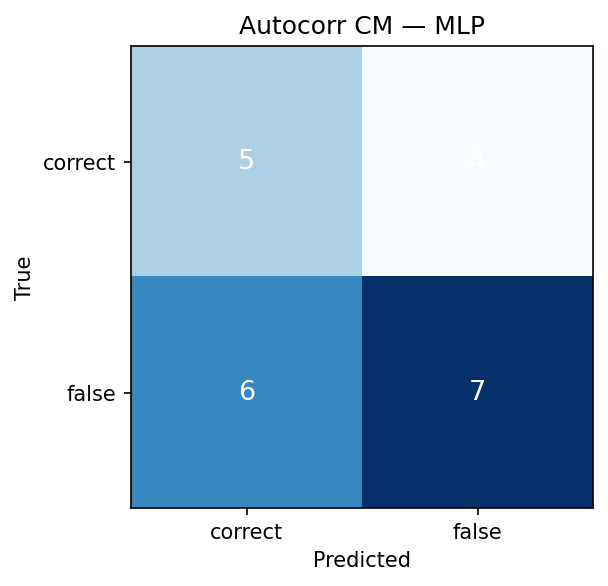
\includegraphics[width=0.65\textwidth]{figures/autocorr_confusion_matrix.png}
\caption[Confusion matrix for autocorr-based landmark pipeline on test split.]{Confusion matrix for the autocorrelation-based landmark pipeline on the controlled test split.}
\label{fig:autocorr-confusion-matrix}
\end{figure}
}{}

% ---------------------------------------------------------------------
\section{Handmade versus Autocorr Comparison}
\label{sec:hm-vs-ac}
% Source file: figures/main_pipeline_comparison.csv

Table~\ref{tab:hm-ac} gives the main controlled comparison between clean
manual cycles and automatic autocorrelation cycles. The rows use the same
landmark representation family, so the comparison isolates the effect of cycle
source.

\begin{table}[htbp]
\centering
\caption[Main comparison between handmade upper bound and autocorr baseline. Source: \protect\path{main_pipeline_comparison.csv}.]{Main comparison between handmade upper bound and autocorr automatic landmark baseline. Best controlled result in bold. Source: \path{main_pipeline_comparison.csv}.}
\label{tab:hm-ac}
\small
% Sử dụng tabularx với cột X đầu tiên giúp tự động xuống dòng các tên Pipeline quá dài
\begin{tabularx}{\textwidth}{X l r r r r r}
\toprule
\textbf{Pipeline} & \textbf{Cycle source} & \textbf{Test acc.} & \textbf{Macro-F1} & \textbf{F1-correct} & \textbf{F1-false} & \textbf{ROC-AUC} \\
\midrule
Handmade landmark upper bound & Manual & \textbf{0.9107} & \textbf{0.8991} & \textbf{0.9333} & \textbf{0.8649} & \textbf{0.9556} \\
\addlinespace
Autocorr landmark baseline & Automatic & 0.5455 & 0.5417 & 0.5000 & 0.5833 & 0.6068 \\
\bottomrule
\end{tabularx}
\end{table}

Replacing handmade cycles with automatic cycles reduces accuracy by
0.3652 (from 0.9107 to 0.5455) and macro-F1 by 0.3574 (from 0.8991 to 0.5417).
Because both pipelines share the same landmark representation, classifier
family, split, and reporting protocol, this gap is attributable primarily to
the cycle-segmentation stage rather than to the classifier. This is the
central empirical finding of the thesis: the markerless representation is
\emph{learnable} (Section~\ref{sec:handmade}) but the automatic
\emph{segmentation} of in-the-wild running cycles is the dominant bottleneck.
The detection-stage statistics also show why: the
\texttt{contact\_diff} pipeline retains only 151 of its raw cycles and fails
to detect usable cycles in a substantial number of videos
(Section~\ref{sec:signal-ablation}). Section~\ref{sec:fair-gap} tests the
same interpretation under repeated video-level folds.

\begin{figure}[htbp]
\centering
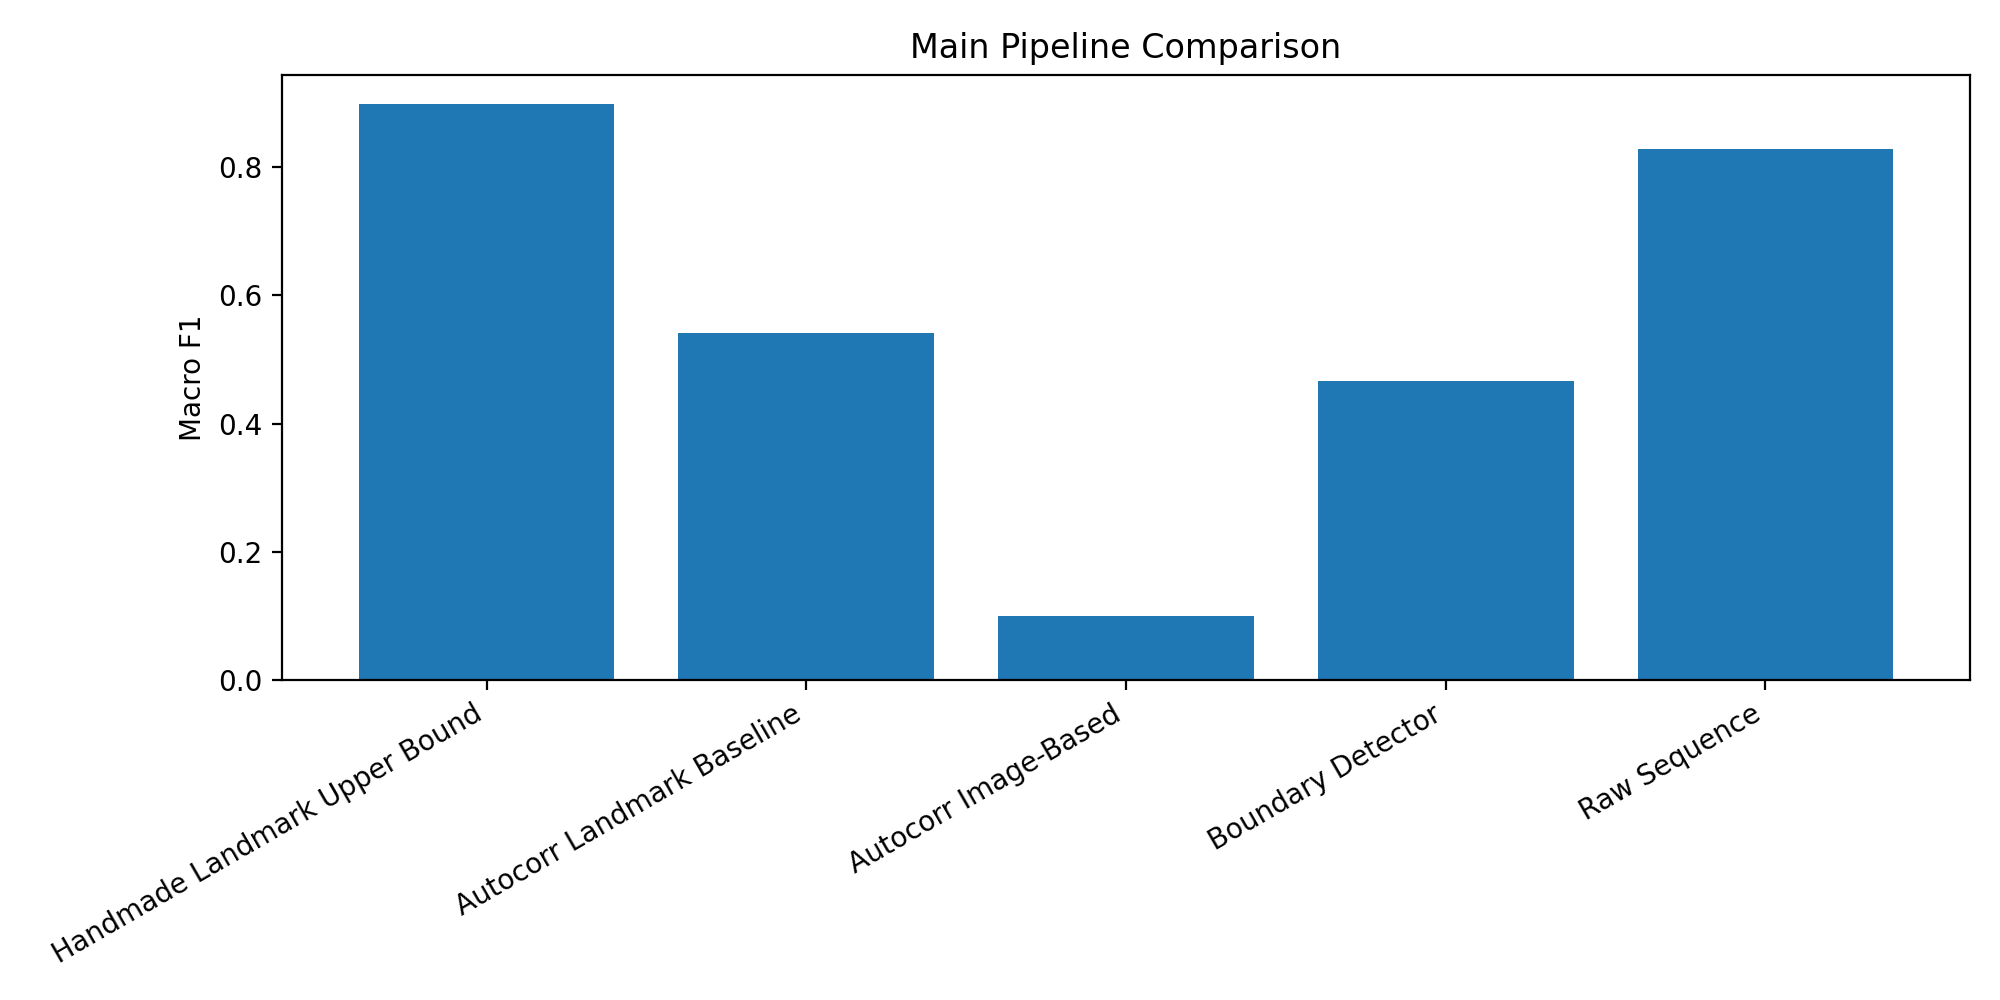
\includegraphics[width=0.85\textwidth]{figures/main_pipeline_comparison.png}
\caption[Main pipeline comparison. Source: \protect\path{main_pipeline_comparison.png}.]{Main pipeline comparison between the handmade landmark upper bound, the autocorr landmark baseline, and supplementary pipelines. Source: \path{main_pipeline_comparison.png}.}
\label{fig:main-pipeline-comparison}
\end{figure}


% ---------------------------------------------------------------------
\section{Fair Gap Robustness Check}
\label{sec:fair-gap}

The fixed-split comparison in Section~\ref{sec:hm-vs-ac} gives the primary
controlled benchmark, but the validation and test sets are small. To test
whether the handmade--autocorr gap was merely a difficult split artefact, an
additional fair-gap robustness check was conducted. Both cycle sources were
evaluated using the same MLP classifier, 5-fold video-level cross-validation,
a fixed threshold of $0.5$, and macro-F1 as the main metric.

\begin{table}[htbp]
\centering
\caption[Fair-gap robustness check under 5-fold video-level CV. Source: \protect\path{fair_gap_and_mlp_perm.csv}.]{Fair-gap robustness check under 5-fold video-level cross-validation using the same MLP classifier and threshold $0.5$. Source: \path{outputs/autocorr/fair_gap_and_mlp_perm.csv}.}
\label{tab:fair-gap-cv}
\small
\begin{tabularx}{\textwidth}{X r r r l}
\toprule
\textbf{Cycle source} & \textbf{Cycles} & \textbf{Videos} & \textbf{CV macro-F1} & \textbf{OOF macro-F1, 95\% CI} \\
\midrule
Handmade cycles & 370 & 369 & $0.860 \pm 0.016$ & $0.860$ [0.822, 0.897] \\
Autocorr cycles & 151 & 55  & $0.615 \pm 0.081$ & $0.655$ [0.580, 0.728] \\
\midrule
\multicolumn{3}{l}{\textbf{Fair gap (handmade $-$ autocorr)}} & \textbf{0.245} & -- \\
\bottomrule
\end{tabularx}
\end{table}

Table~\ref{tab:fair-gap-cv} confirms the same conclusion as the fixed-split
benchmark. Handmade cycles remain stable under repeated video-level folds,
achieving $0.860 \pm 0.016$ macro-F1. Autocorr cycles remain substantially
weaker, achieving $0.615 \pm 0.081$ macro-F1. The resulting fair gap of 0.245
macro-F1 is smaller than the single fixed-split gap of 0.3574, but it remains
large enough to show that the performance loss is systematic rather than only
the result of one difficult split.

A permutation test was then applied to the autocorr MLP setting to assess
whether the observed autocorr features were robustly separable under the same
simple classifier. With 100 random label permutations, the observed CV macro-F1
was 0.5206, while the null distribution had a mean of 0.468 and a standard
deviation of 0.074, giving $p = 0.2475$. This does not establish statistically
significant separation from the permutation baseline. The result should be read
conservatively: autocorr-derived cycles contain some discriminative signal, as
also reflected by the CV comparison, but the signal is noisy and not robustly
separable under the tested MLP configuration.

\begin{table}[htbp]
\centering
\caption[Permutation test for the autocorr MLP setting. Source: \protect\path{fair_gap_and_mlp_perm.json}.]{Permutation test for the autocorr MLP setting. Source: \path{outputs/autocorr/fair_gap_and_mlp_perm.json}.}
\label{tab:autocorr-permutation}
\small
\begin{tabularx}{\textwidth}{X r}
\toprule
\textbf{Quantity} & \textbf{Value} \\
\midrule
Observed autocorr CV macro-F1 & 0.5206 \\
Null mean macro-F1 & 0.4680 \\
Null standard deviation & 0.0740 \\
Number of permutations & 100 \\
Permutation $p$-value & 0.2475 \\
\bottomrule
\end{tabularx}
\end{table}


% ---------------------------------------------------------------------
\section{Model Ablation Results}
\label{sec:model-ablation}
% Source file: outputs/ablation/model_ablation.csv

The model ablation compares MLP, 1D-CNN, BiLSTM, and CNN-BiLSTM architectures
under the handmade and autocorr pipelines. Table~\ref{tab:model-ablation}
shows the macro-F1 and accuracy for each setting.

\begin{table}[htbp]
\centering
\caption[Model ablation on handmade and autocorr pipelines. Source: \protect\path{model_ablation.csv}.]{Model ablation on handmade and autocorr pipelines. Best macro-F1 within each pipeline in bold. Source: \path{model_ablation.csv}.}
\label{tab:model-ablation}
\small
\begin{tabular}{llrrr}
\toprule
Pipeline & Model & Test acc. & Macro-F1 & ROC-AUC \\
\midrule
\multirow{4}{*}{Handmade}
& MLP & 0.8571 & 0.8545 & 0.9444 \\
& 1D-CNN & 0.8929 & 0.8772 & 0.9444 \\
& BiLSTM & 0.8750 & 0.8623 & \textbf{0.9556} \\
& CNN-BiLSTM & \textbf{0.9107} & \textbf{0.8991} & \textbf{0.9556} \\
\midrule
\multirow{4}{*}{Autocorr}
& MLP & 0.5455 & 0.5417 & 0.6068 \\
& 1D-CNN & 0.5000 & 0.3425 & 0.5684 \\
& BiLSTM & 0.4545 & 0.3714 & 0.5342 \\
& CNN-BiLSTM & \textbf{0.5909} & \textbf{0.5901} & \textbf{0.6370} \\
\bottomrule
\end{tabular}
\end{table}

The architecture effect is pipeline-dependent. In the handmade setting, the
hybrid CNN-BiLSTM performs best, suggesting that local pose patterns and
temporal ordering are both useful when the eight phases are correctly aligned.
In the automatic setting, model ranking becomes unstable: at a 0.5 threshold the CNN-BiLSTM is best (macro-F1 0.5901), whereas the
simpler MLP wins once thresholds are tuned (Section~\ref{sec:threshold}). The
absolute values remain low for every automatic-pipeline model, reinforcing
that architecture choice cannot recover the information lost to imperfect
segmentation.

% ---------------------------------------------------------------------
\section{Feature Ablation Results}
\label{sec:feature-ablation}
% Source file: outputs/ablation/feature_ablation.csv

The feature ablation fixes the classifier and varies only the input feature
set, on the handmade pipeline. Table~\ref{tab:feature-ablation} reports the
resulting performance.

\begin{table}[htbp]
\centering
\caption[Feature ablation on handmade cycles. Source: \protect\path{feature_ablation.csv}.]{Feature ablation on handmade cycles. Best macro-F1 in bold. Source: \path{feature_ablation.csv}.}
\label{tab:feature-ablation}
\small
\begin{tabular}{lrrrr}
\toprule
Feature set & Test acc. & Macro-F1 & F1-false & ROC-AUC \\
\midrule
Selected 13 landmarks & 0.9107 & \textbf{0.8991} & 0.8649 & \textbf{0.9556} \\
All 33 landmarks & 0.8929 & 0.8961 & \textbf{0.9189} & 0.9389 \\
Lower-body only & 0.8929 & 0.8961 & \textbf{0.9189} & 0.9222 \\
Selected 13 + velocity & 0.9107 & \textbf{0.8991} & 0.8649 & \textbf{0.9556} \\
\bottomrule
\end{tabular}
\end{table}

The selected 13-landmark representation matches the best macro-F1 while
remaining lower-dimensional than the full 33-landmark representation. The
lower-body-only and all-landmark variants improve F1-false but do not improve
macro-F1 overall, suggesting that additional coordinates can alter class
balance without yielding a more robust classifier. The selected-landmark
configurations cluster tightly around 0.90~macro-F1, supporting the use of the
compact 13-landmark representation as the pipeline default for the automatic
experiments, where added input dimensionality offers little benefit relative
to its sensitivity to landmark noise.

% ---------------------------------------------------------------------
\section{Signal Ablation Results}
\label{sec:signal-ablation}
% Source file: outputs/ablation/signal_ablation.csv

The signal ablation compares the seven candidate motion signals used for
cycle detection, holding the classifier family fixed. Table~\ref{tab:signal}
reports detection coverage and classification performance.

\begin{table}[htbp]
\centering
\caption[Cycle-detection signal ablation. Source: \protect\path{signal_ablation.csv}.]{Cycle-detection signal ablation. Best macro-F1 and best retained cycle count are bolded separately. Source: \path{signal_ablation.csv}.}
\label{tab:signal}
\small
\begin{tabular}{lrrrrr}
\toprule
Signal & Test acc. & Macro-F1 & Videos OK & Cycles retained & Cycles rejected \\
\midrule
head\_y & 0.6818 & 0.6703 & \textbf{72} & \textbf{204} & 13 \\
hip\_y & \textbf{0.7333} & \textbf{0.7321} & 67 & 190 & 15 \\
heel\_y & 0.6667 & 0.6623 & 35 & 49 & 36 \\
toe\_y & 0.5000 & 0.5000 & 35 & 52 & 33 \\
contact\_diff & 0.5909 & 0.5901 & 50 & 151 & 42 \\
AP\_diff & 0.2500 & 0.2000 & 32 & 33 & 39 \\
V\_diff & 0.6364 & 0.6022 & 48 & 125 & 34 \\
\bottomrule
\end{tabular}
\end{table}

The \texttt{hip\_y} signal achieves the highest classification macro-F1 in this
ablation, while \texttt{contact\_diff} is retained as the main baseline signal
because it reflects foot-contact dynamics and produces more semantically
aligned cycle boundaries. The decision is not based on accuracy alone. In this
thesis, the baseline signal must support foot-strike-to-foot-strike sampling,
eight-phase interpretation, and stable comparison to the image pipeline. The
\texttt{contact\_diff} signal therefore produces the most temporally coherent
foot-strike-to-foot-strike boundaries, consistent with periodic gait-cycle structure in human motion \cite{cutting1978gaitperiodicity,plotnik2007gaitasymmetry}, which is why it is adopted as the
baseline cycle-detection signal even though its classification macro-F1
(0.5901) is not the single highest. The vertical signals
(\texttt{head\_y}, \texttt{hip\_y}) detect more videos but admit many
ill-formed cycles, illustrating the trade-off between detection coverage and
boundary precision that underlies the segmentation bottleneck identified in
Section~\ref{sec:hm-vs-ac}.

% ---------------------------------------------------------------------
\section{Frames-per-Cycle Ablation Results}
\label{sec:frames-ablation}
% Source file: outputs/ablation/frames_ablation.csv

The frame ablation tests whether increasing temporal resolution beyond the
eight-phase representation improves performance on handmade cycles. Table~\ref{tab:frames} summarises the best model at each frame count.

\begin{table}[htbp]
\centering
\caption[Frames-per-cycle ablation on handmade cycles. Source: \protect\path{frames_ablation.csv}.]{Frames-per-cycle ablation on handmade cycles. Best macro-F1 in bold. Source: \path{frames_ablation.csv}.}
\label{tab:frames}
\small
\begin{tabular}{lrrrr}
\toprule
Frames per cycle & Best model & Test acc. & Macro-F1 & ROC-AUC \\
\midrule
8 & CNN-BiLSTM & 0.9107 & \textbf{0.8991} & \textbf{0.9556} \\
16 & BiLSTM & 0.8750 & 0.8623 & \textbf{0.9556} \\
24 & CNN-BiLSTM & 0.8393 & 0.8347 & 0.9389 \\
32 & CNN-BiLSTM & 0.8571 & 0.8545 & 0.9444 \\
\bottomrule
\end{tabular}
\end{table}

The eight-phase representation gives the best macro-F1 despite being the
shortest sequence. Sixteen frames remain highly competitive
(BiLSTM macro-F1 0.8623 at the lowest cost), and increasing frame count
yields no monotonic improvement. This supports the eight-phase sampling
choice as an efficient representation of the running cycle, with additional
temporal resolution providing diminishing returns on this dataset.

% ---------------------------------------------------------------------
\section{Autocorr Version History and Method Evolution}
\label{sec:version-history}
% Source file: figures/autocorr_version_comparison.csv

This section documents the evolution of the autocorrelation pipeline. The
values in Table~\ref{tab:version-history} are \emph{historical} validation
figures drawn from development notebooks; they are presented as method-evolution
evidence only and must not be read as controlled benchmark results. Where a
metric was never recorded under the controlled protocol it is marked
\texttt{[MISSING RESULT]}.

\begin{table}[htbp]
\centering
\caption[Autocorr version history and development evidence.]{Autocorr version history (historical development evidence --- not a controlled benchmark). Source: \protect\path{autocorr_version_comparison.csv}.}
\label{tab:version-history}
\footnotesize
\begin{tabularx}{\textwidth}{l X l X r}
\toprule
\textbf{Version} & \textbf{Signal} & \textbf{Input} & \textbf{Model} & \textbf{Val. acc. (\%)} \\
\midrule
\texttt{autocorr\_fixed\_val\_acc\_69\_6} & head-Y oscillation & landmarks & CNN+LSTM & 69.6 \\
\addlinespace
% SỬA LỖI DÒNG 161+ TẠI ĐÂY: Thêm dấu escape \% ở 69.6\%, 72.9\%, 76.5\% để không bị lỗi Missing $
\texttt{autocorr\_fixed\_val\_acc\_72\_9} & \texttt{contact\_diff} & landmarks & CNN+LSTM & 72.9 \\
\addlinespace
\texttt{autocorr\_fixed\_biLSTM} & \texttt{contact\_diff} & landmarks $+$ vel. & BiLSTM & 65.0 \\
\addlinespace
\texttt{autocorr\_fixed\_val\_acc\_76\_5} & \texttt{contact\_diff} & RGB crop $224^2$ & MobileNetV2$+$LSTM & 76.5 \\
\midrule
\texttt{02\_baseline\_landmark} & \texttt{contact\_diff} & 13 lm $+$ vel. & best of 4 & \multicolumn{1}{c}{$^{\dagger}$} \\
\bottomrule
\end{tabularx}
\end{table}

\begin{figure}[htbp]
\centering
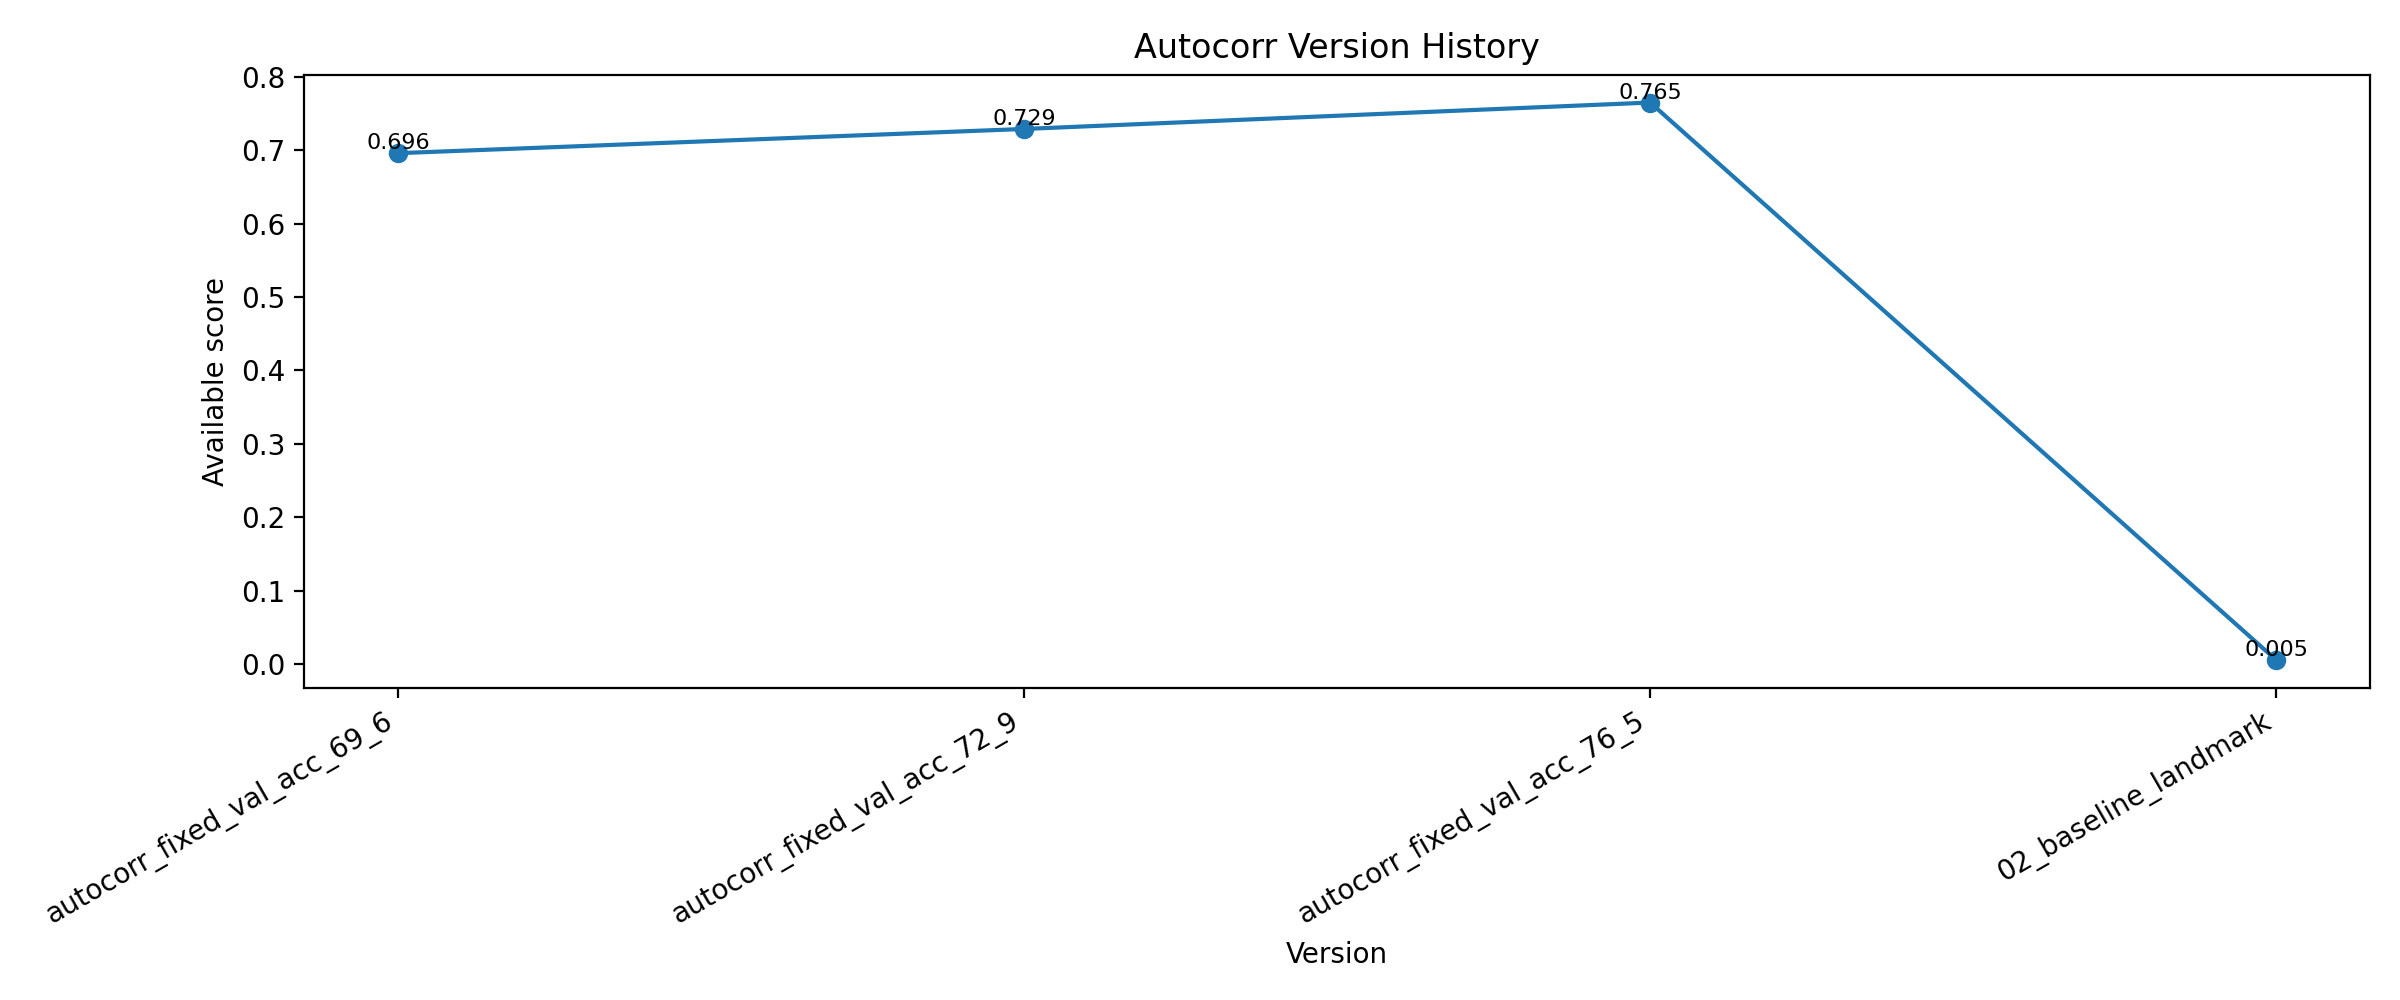
\includegraphics[width=0.85\textwidth]{figures/autocorr_version_history.png}
\caption[Historical autocorr method evolution.]{Historical autocorr method evolution. This figure is development evidence only; Source: \path{autocorr_version_history.png}.}
\label{fig:autocorr-version-history}
\end{figure}

\noindent$^{\dagger}$ The \texttt{02\_baseline\_landmark} row is the only
controlled entry; under the fixed-split protocol it records a test accuracy of
0.5455 and a test macro-F1 of 0.5417 (Section~\ref{sec:autocorr-baseline}), in
[0,1] rather than percent. Its historical validation accuracy was not recorded
(\texttt{[MISSING RESULT]}).

The development trace shows three substantive changes: replacing the noisy
head-Y oscillation signal with \texttt{contact\_diff} (historical validation
69.6\% $\rightarrow$ 72.9\%), adopting autocorrelation period estimation with
foot-strike-to-foot-strike alignment, and an exploratory shift to an
image-based representation (\texttt{autocorr\_fixed\_val\_acc\_76\_5}). The
76.5\% figure is the most technically complex historical milestone, but it is
a development validation accuracy on an RGB-crop representation and was not
re-confirmed under the controlled protocol; it is therefore retained as
motivation for the organised image-based rerun
(Section~\ref{sec:image-results}) rather than as evidence that image-based
modelling outperforms the landmark baseline.

% ---------------------------------------------------------------------
\section{Autocorr Image-Based Results}
\label{sec:image-results}
% Source file: outputs/autocorr_image/image_results.csv

The image-based pipeline is the \emph{controlled} rerun of the historical
image idea: it reuses the exact \texttt{contact\_diff}/autocorrelation cycle
source of the landmark baseline, but represents each phase as a runner-centred
RGB crop processed by a MobileNetV2$+$LSTM model \cite{sandler2018mobilenetv2,hochreiter1997lstm,donahue2015lrcn}. Table~\ref{tab:image}
reports the controlled result.

\begin{table}[htbp]
\centering
\caption[Autocorr image-based pipeline results. Source: \protect\path{image_results.csv}.]{Autocorr image-based pipeline (controlled rerun). Source: \path{image_results.csv}.}
\label{tab:image}
\small
\begin{tabular}{llrrrr}
\toprule
Input & Model & Test acc. & Macro-F1 & F1-false & ROC-AUC \\
\midrule
RGB crop & MobileNetV2$+$LSTM & 0.1111 & 0.1000 & 0.2000 & 0.0592 \\
\bottomrule
\end{tabular}
\end{table}

Under the controlled protocol the image-based pipeline reaches a test macro-F1
of only 0.1000, with F1-correct of 0.0000 and a ROC-AUC of 0.0592, i.e.\ far
below chance. The model effectively fails to learn a usable decision boundary
on this small dataset. Crucially, this controlled result does \emph{not}
reproduce the historical 76.5\% validation figure of
Section~\ref{sec:version-history}, which underscores why that figure cannot
serve as a benchmark. The collapse is consistent with the known fragilities of
the image representation on limited in-the-wild data: bounding-box and crop
instability, domain shift, and overfitting of a high-capacity visual backbone \cite{sandler2018mobilenetv2}.
This indicates that the current image-based implementation
is not yet stable enough to replace the landmark baseline, not that image-based
modelling is invalid in principle.

\IfFileExists{figures/image_confusion_matrix.png}{%
\begin{figure}[htbp]
\centering
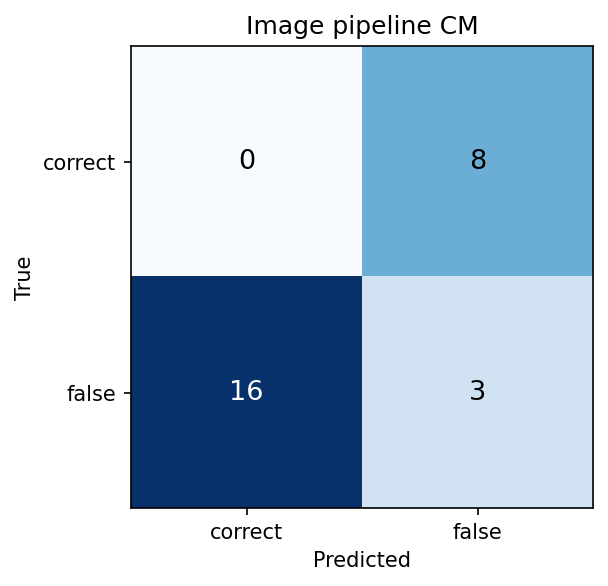
\includegraphics[width=0.65\textwidth]{figures/image_confusion_matrix.png}
\caption[Confusion matrix for the image-based pipeline.]{Confusion matrix for the image-based pipeline on the controlled test split.}
\label{fig:image-confusion-matrix}
\end{figure}
}{}

% ---------------------------------------------------------------------
\section{Landmark-Based versus Image-Based Representation}
\label{sec:representation}
% Source file: figures/representation_comparison.csv
%              (video-level: representation_video_level_comparison.csv)

Table~\ref{tab:repr} compares the two representations on the same automatic
cycle source, at the cycle (sample) level.

\begin{table}[htbp]
\centering
\caption[Landmark vs image representation. Source: \protect\path{representation_comparison.csv}.]{Landmark versus image representation (controlled), identical cycle source. Source: \path{representation_comparison.csv}.}
\label{tab:repr}
\small
\begin{tabular}{llrrrr}
\toprule
Representation & Model & Test acc. & Macro-F1 & ROC-AUC & Test samples \\
\midrule
Landmark & MLP & \textbf{0.5455} & \textbf{0.5417} & 0.6068 & 22 \\
Image & MobileNetV2$+$LSTM & 0.1111 & 0.1000 & 0.0592 & 27 \\
\bottomrule
\end{tabular}
\end{table}

On a matched cycle source, the landmark representation clearly outperforms the
image representation (macro-F1 0.5417 versus 0.1000).The same ordering holds at the video level, where the landmark pipeline reaches 0.6250 accuracy / 0.6190 macro-F1 under majority voting against 0.2857 / 0.2222 for the image pipeline (\path{representation_video_level_comparison.csv}).
For this dataset and
implementation, the sparse landmark sequence is the more reliable
representation; the RGB-crop pipeline does not add usable discriminative
information and is markedly less stable. This addresses the
representation research question while remaining within the controlled
protocol, separately from the historical 76.5\% milestone.

\begin{figure}[htbp]
\centering
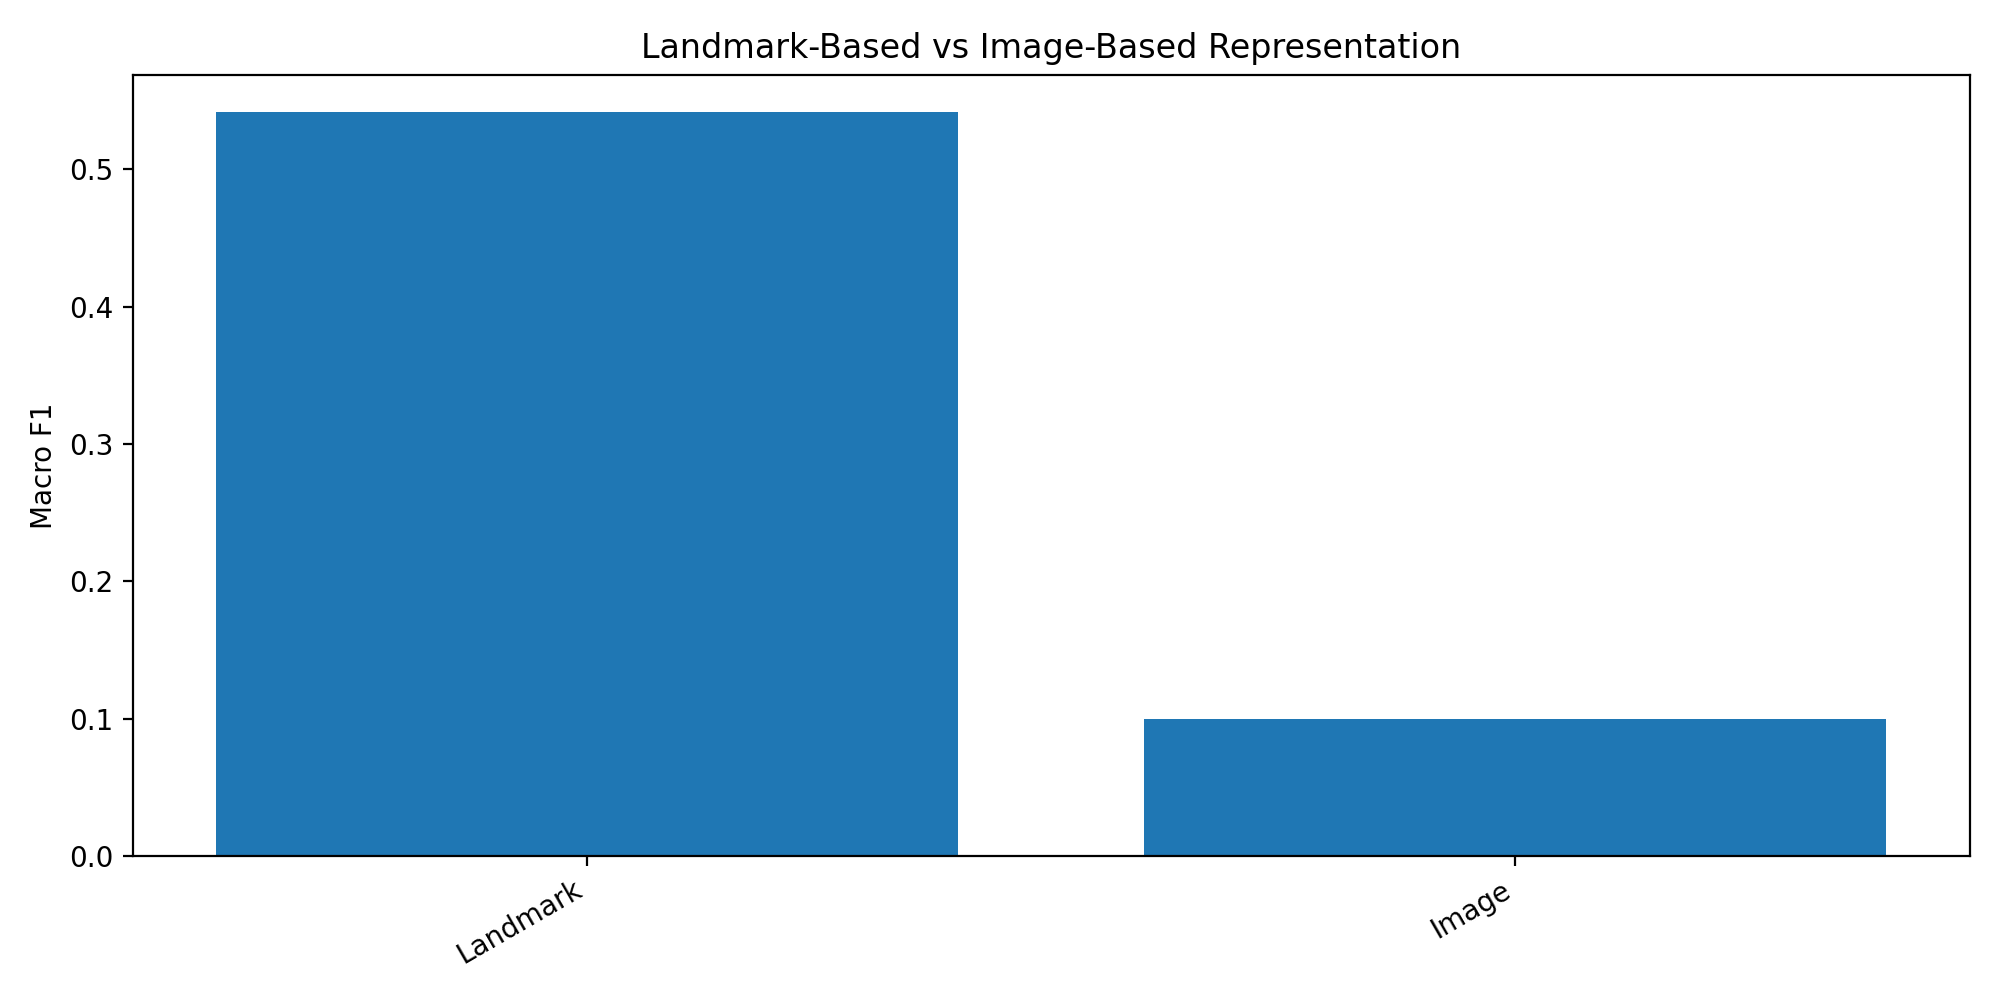
\includegraphics[width=0.85\textwidth]{figures/landmark_vs_image_comparison.png}
\caption[Controlled landmark-versus-image comparison.]{Controlled landmark-versus-image representation comparison under the automatic autocorr cycle source. Source: \path{landmark_vs_image_comparison.png}.}
\label{fig:landmark-vs-image-comparison}
\end{figure}

% ---------------------------------------------------------------------
\section{Cycle-Level versus Video-Level Evaluation}
\label{sec:cycle-vs-video}
% Source files: figures/cycle_level_metrics.csv,
%               figures/video_level_metrics.csv

Because each video may yield several cycles, predictions can be reported per
cycle or aggregated per video. Table~\ref{tab:cyc-vid} compares the two for the
automatic landmark baseline (the main pipeline) and lists the supplementary
pipelines for reference.

\begin{table}[htbp]
\centering
\caption[Cycle-level versus video-level evaluation.]{Cycle-level versus video-level evaluation. Video-level uses majority vote. Sources: \protect\path{cycle_level_metrics.csv}, \protect\path{video_level_metrics.csv}.}
\label{tab:cyc-vid}
\small
\begin{tabular}{llrrrr}
\toprule
Pipeline & Level & Acc. & Macro-F1 & F1-false & $N$ \\
\midrule
\multirow{2}{*}{Autocorr (baseline)}
& Cycle & 0.5238 & 0.5139 & 0.5833 & 21 \\
& Video (majority) & \textbf{0.5714} & \textbf{0.5333} & 0.6667 & 7 \\
\midrule
Image & Cycle & 0.1111 & 0.1000 & 0.2000 & 27 \\
Image & Video (majority) & 0.2857 & 0.2222 & 0.4444 & 7 \\
\midrule
Boundary Detector & Cycle & 0.6000 & 0.5833 & 0.5000 & 5 \\
Boundary Detector & Video (majority) & 0.6667 & 0.6667 & 0.6667 & 3 \\
\midrule
Raw sequence & Cycle/Video & 0.8182 & 0.8036 & 0.8571 & 11 \\
\bottomrule
\end{tabular}
\end{table}

For the automatic landmark baseline, aggregating cycle predictions to the video
level by majority vote improves both accuracy (0.5238 $\rightarrow$ 0.5714) and
macro-F1 (0.5139 $\rightarrow$ 0.5333). The same direction appears for the image
and boundary-detector pipelines. This indicates that per-cycle predictions
contain noise that partially cancels under aggregation, so video-level reporting
gives a fairer estimate of practical performance. The very
small video counts ($N=3$--$7$) mean these gains, while consistent in
direction, rest on few samples and should be treated as indicative.

\begin{figure}[htbp]
\centering
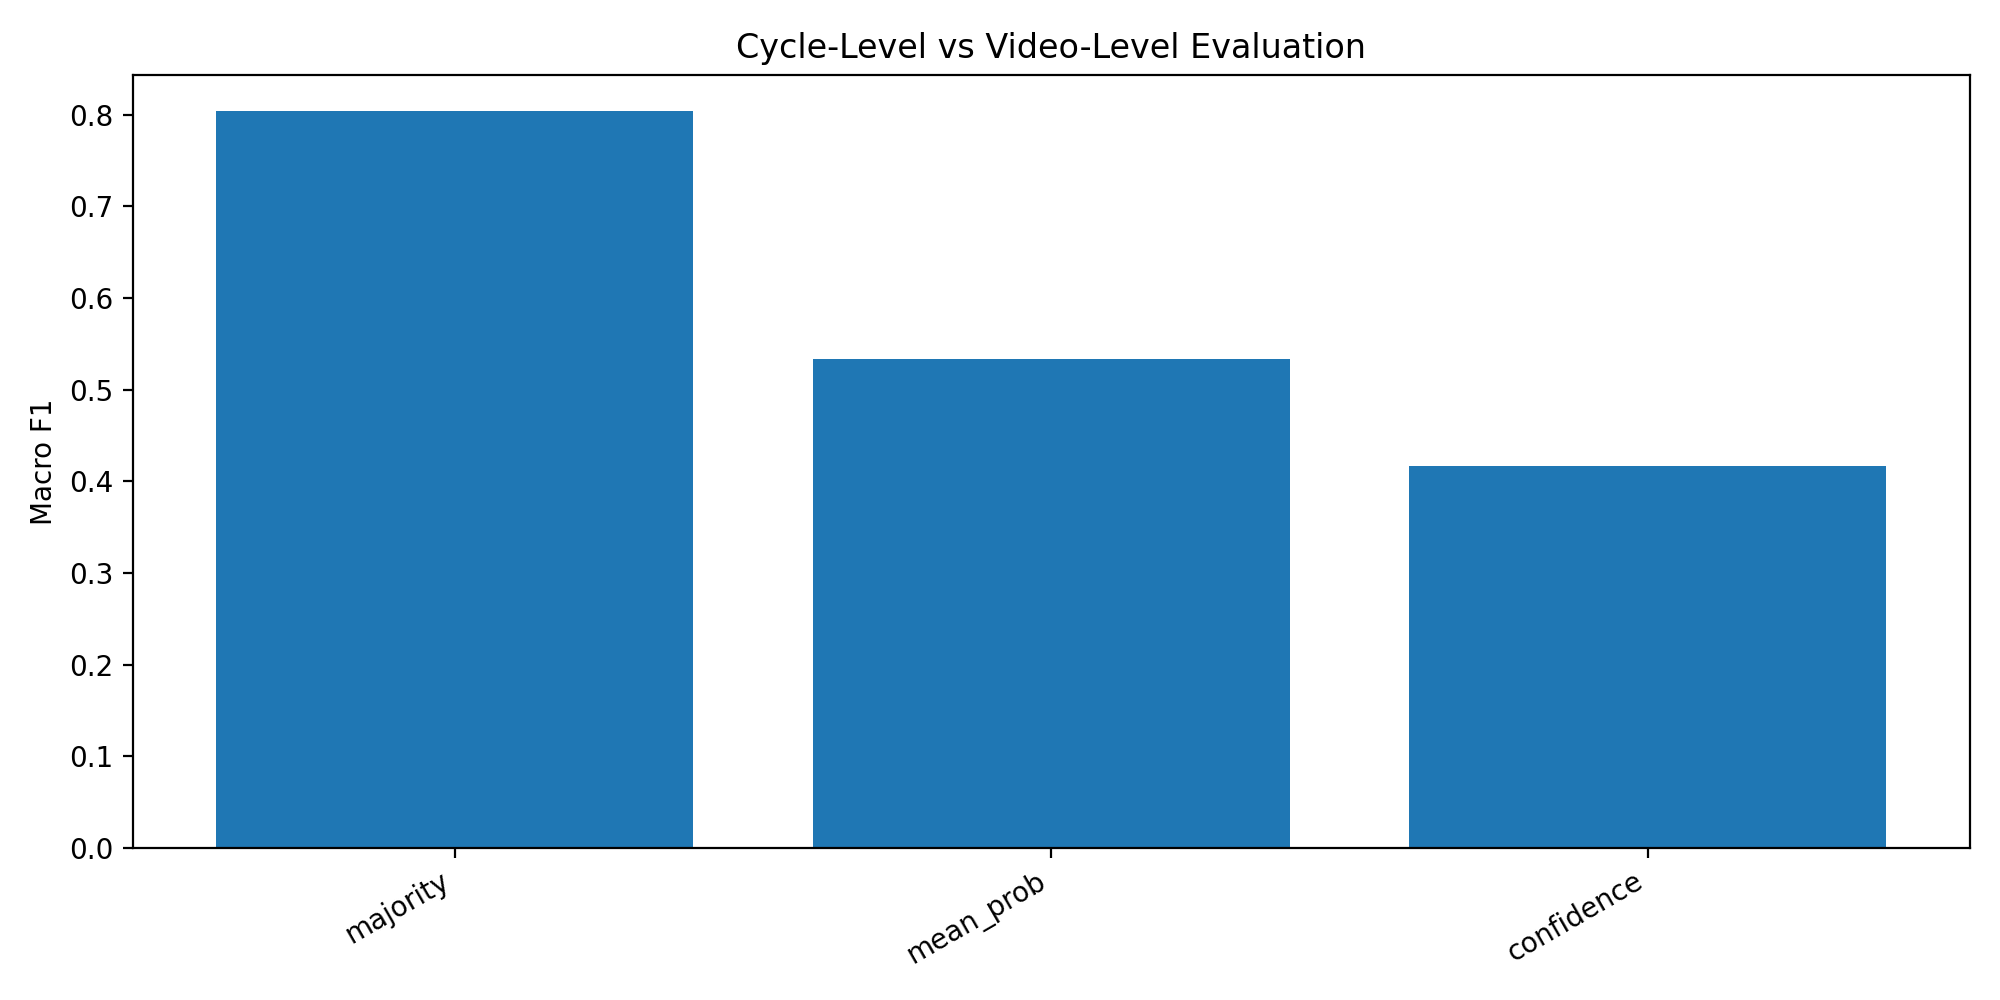
\includegraphics[width=0.85\textwidth]{figures/cycle_vs_video_comparison.png}
\caption[Cycle-level versus video-level evaluation.]{Cycle-level versus video-level evaluation. Video-level predictions aggregate cycle predictions by majority voting. Source: \path{cycle_vs_video_comparison.png}.}
\label{fig:cycle-vs-video-comparison}
\end{figure}

% ---------------------------------------------------------------------
\section{Threshold 0.5 versus Tuned Threshold}
\label{sec:threshold}
% Source file: figures/threshold_05_vs_tuned.csv

Decision thresholds tuned on validation can either improve or overfit test
performance. Table~\ref{tab:threshold} reports, for each model, the macro-F1 at
the default 0.5 threshold and at the validation-selected threshold, together
with the change and an overfit flag.

\begin{table}[htbp]
\centering
\caption[Default threshold versus validation-tuned threshold.]{Default threshold versus validation-tuned threshold. Thresholds are selected on validation and applied to test. Source: \protect\path{threshold_05_vs_tuned.csv}.}
\label{tab:threshold}
\tablefont
\begin{adjustbox}{max width=\textwidth}
\begin{tabular}{llrrrrl}
\toprule
Pipeline & Model & Macro-F1@0.5 & Best thr. & Tuned macro-F1 & $\Delta$ & Overfit \\
\midrule
\multirow{4}{*}{Handmade}
& 1D-CNN & 0.8961 & 0.34 & 0.8772 & $-0.0189$ & True \\
& BiLSTM & 0.8772 & 0.78 & 0.8772 & $0.0000$ & False \\
& CNN-BiLSTM & 0.8772 & 0.40 & \textbf{0.8991} & $+0.0219$ & False \\
& MLP & 0.8250 & 0.16 & 0.8545 & $+0.0295$ & False \\
\midrule
\multirow{4}{*}{Autocorr}
& MLP & 0.5417 & 0.34 & \textbf{0.5417} & $0.0000$ & False \\
& 1D-CNN & 0.3425 & 0.50 & 0.3425 & $0.0000$ & False \\
& BiLSTM & 0.3714 & 0.54 & 0.2903 & $-0.0811$ & True \\
& CNN-BiLSTM & 0.5901 & 0.18 & 0.4359 & $-0.1542$ & True \\
\midrule
Image & all & 0.1000 & \texttt{[MISSING RESULT]} & \texttt{[MISSING RESULT]} & \texttt{[MISSING RESULT]} & False \\
\bottomrule
\end{tabular}
\end{adjustbox}
\end{table}

On the clean handmade pipeline, validation-tuned thresholds mostly help or are
neutral (CNN-BiLSTM improves to 0.8991). On the automatic pipeline the picture
reverses: tuning leaves the MLP unchanged but severely degrades the sequential
models, with the CNN-BiLSTM dropping by 0.1542 macro-F1 and being flagged as
threshold-overfit. This explains the apparent disagreement with the model
ablation (Section~\ref{sec:model-ablation}): the CNN-BiLSTM is best at the 0.5
threshold but unstable once a validation-selected threshold is applied, whereas
the MLP is the robust choice for the reported baseline. The
image pipeline exposes only an aggregate row with no probability-based sweep, so
its tuned entries are \texttt{[MISSING RESULT]}. All reported baseline metrics
state explicitly whether a 0.5 or tuned threshold was used.

\begin{figure}[htbp]
\centering
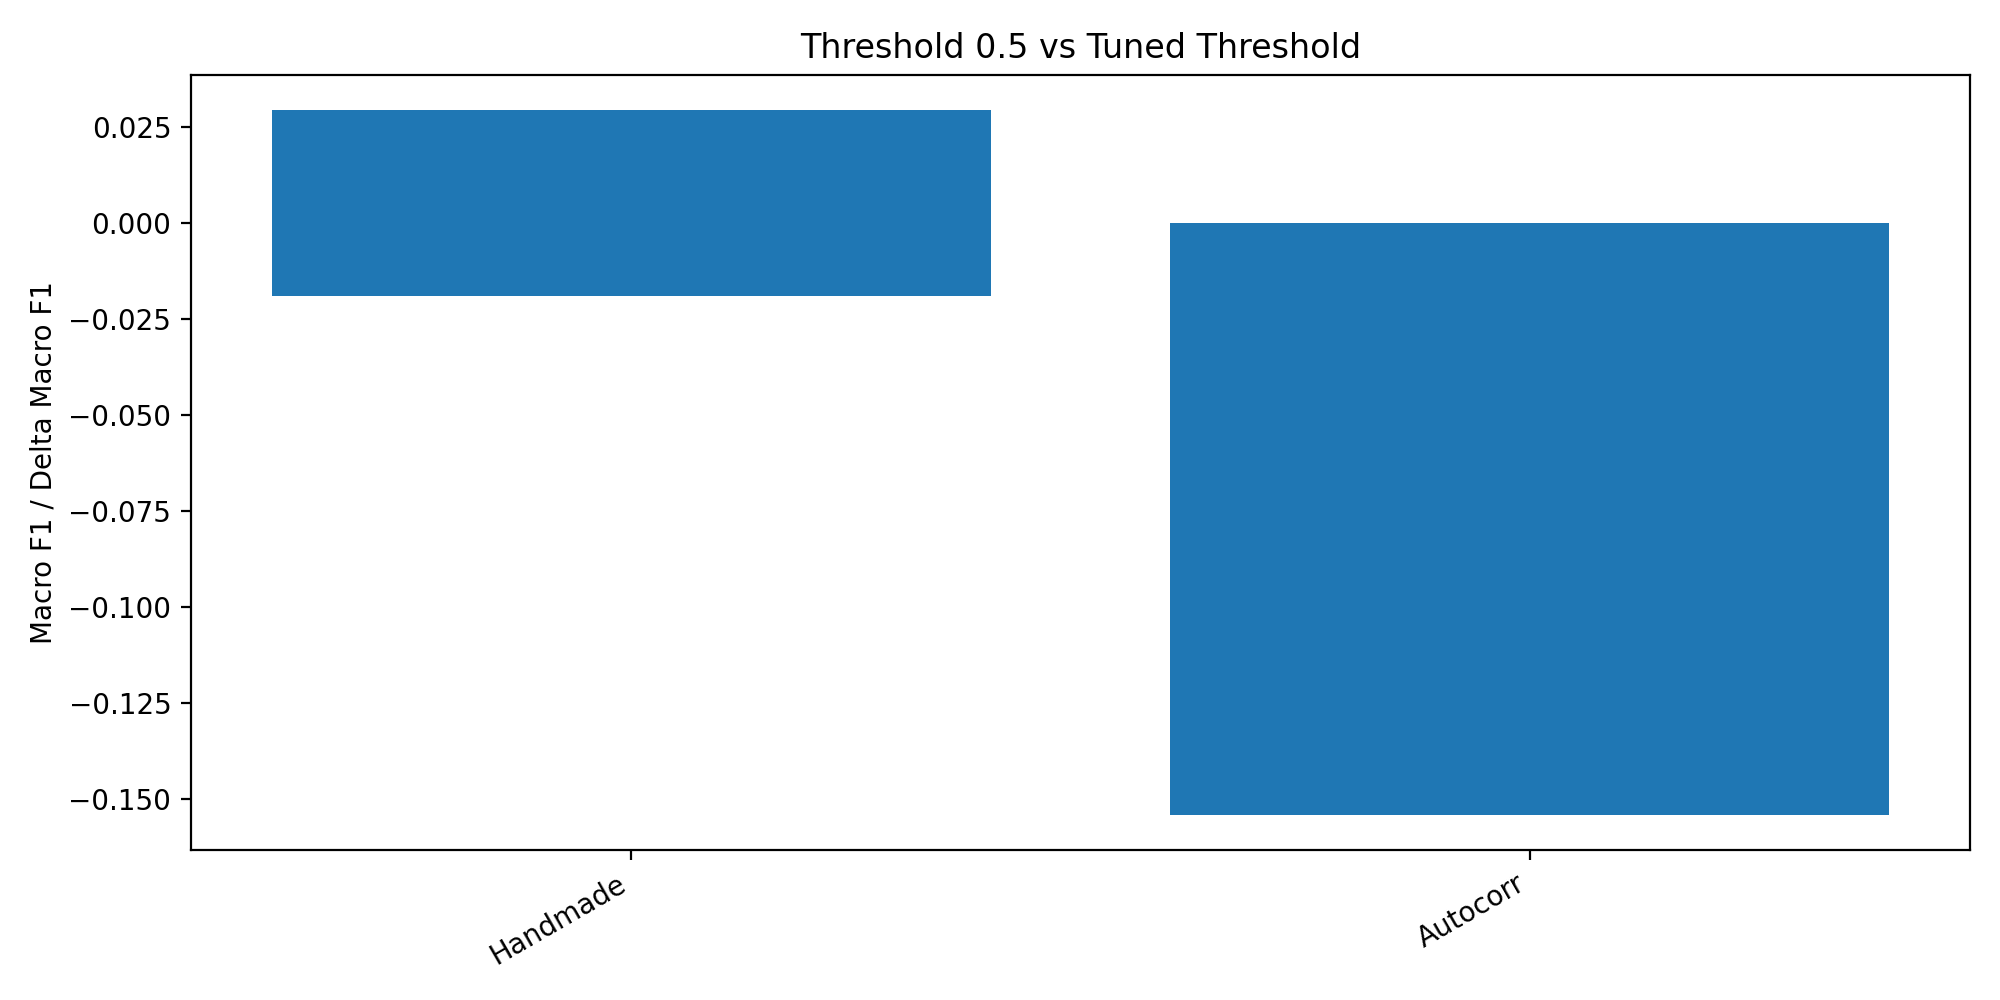
\includegraphics[width=0.85\textwidth]{figures/threshold_comparison.png}
\caption[Comparison between default 0.5 threshold and tuned thresholds.]{Comparison between the default 0.5 decision threshold and validation-tuned thresholds. Source: \path{threshold_comparison.png}.}
\label{fig:threshold-comparison}
\end{figure}

% ---------------------------------------------------------------------
\section{Pose and Cycle Quality Analysis}
\label{sec:quality}
% Source file: figures/pose_cycle_quality_metrics.csv

To locate the source of automatic-pipeline errors, test cycles are grouped by
pose- and cycle-quality factors (median split) and accuracy/macro-F1 compared
across groups. Table~\ref{tab:quality} reports representative factors; within
each factor the higher-accuracy group is bold.

\begin{table}[htbp]
\centering
\caption[Pose and cycle quality analysis (Autocorr baseline).]{Pose and cycle quality analysis (Autocorr baseline). Median-split groups. Source: \protect\path{pose_cycle_quality_metrics.csv}.}
\label{tab:quality}
\small
\begin{tabular}{llrrr}
\toprule
Quality factor & Group & $n$ & Acc. & Macro-F1 \\
\midrule
\multirow{2}{*}{Heel visibility}
& low ($\le 0.91$) & 11 & 0.4545 & 0.4107 \\
& high ($>0.91$) & 11 & \textbf{0.6364} & 0.5417 \\
\midrule
\multirow{2}{*}{Autocorr correlation}
& low ($\le 0.59$) & 18 & 0.5000 & 0.4582 \\
& high ($>0.59$) & 4 & \textbf{0.7500} & 0.4286 \\
\midrule
\multirow{2}{*}{Missing-ratio proxy}
& low ($\le 0.05$) & 11 & \textbf{0.6364} & 0.5417 \\
& high ($>0.05$) & 11 & 0.4545 & 0.4107 \\
\midrule
\multirow{2}{*}{Cycle duration}
& low ($\le 0.88$) & 16 & 0.5000 & 0.4921 \\
& high ($>0.88$) & 6 & \textbf{0.6667} & \textbf{0.6667} \\
\midrule
\multirow{2}{*}{Cycle period}
& low ($\le 0.77$) & 12 & \textbf{0.5833} & 0.5556 \\
& high ($>0.77$) & 10 & 0.5000 & 0.3333 \\
\bottomrule
\end{tabular}
\end{table}

The accuracy trends are consistent with the segmentation-bottleneck
interpretation: cycles with higher heel visibility (0.6364 vs.\ 0.4545), lower
landmark missing-ratio (0.6364 vs.\ 0.4545), and stronger autocorrelation
(0.7500 vs.\ 0.5000) are classified more accurately. In other words, errors
concentrate where pose estimation is unreliable or the periodic signal is weak,
rather than being uniformly distributed. Several
high-quality groups are very small ($n=4$--$6$), so the magnitudes are
indicative; the direction, however, points clearly at upstream pose and cycle
quality as the dominant error source for the automatic pipeline. A complementary
breakdown of failed videos (\texttt{failed\_video\_quality\_summary.csv})
attributes the majority of failures to the cycle-detection stage.

\begin{figure}[htbp]
\centering
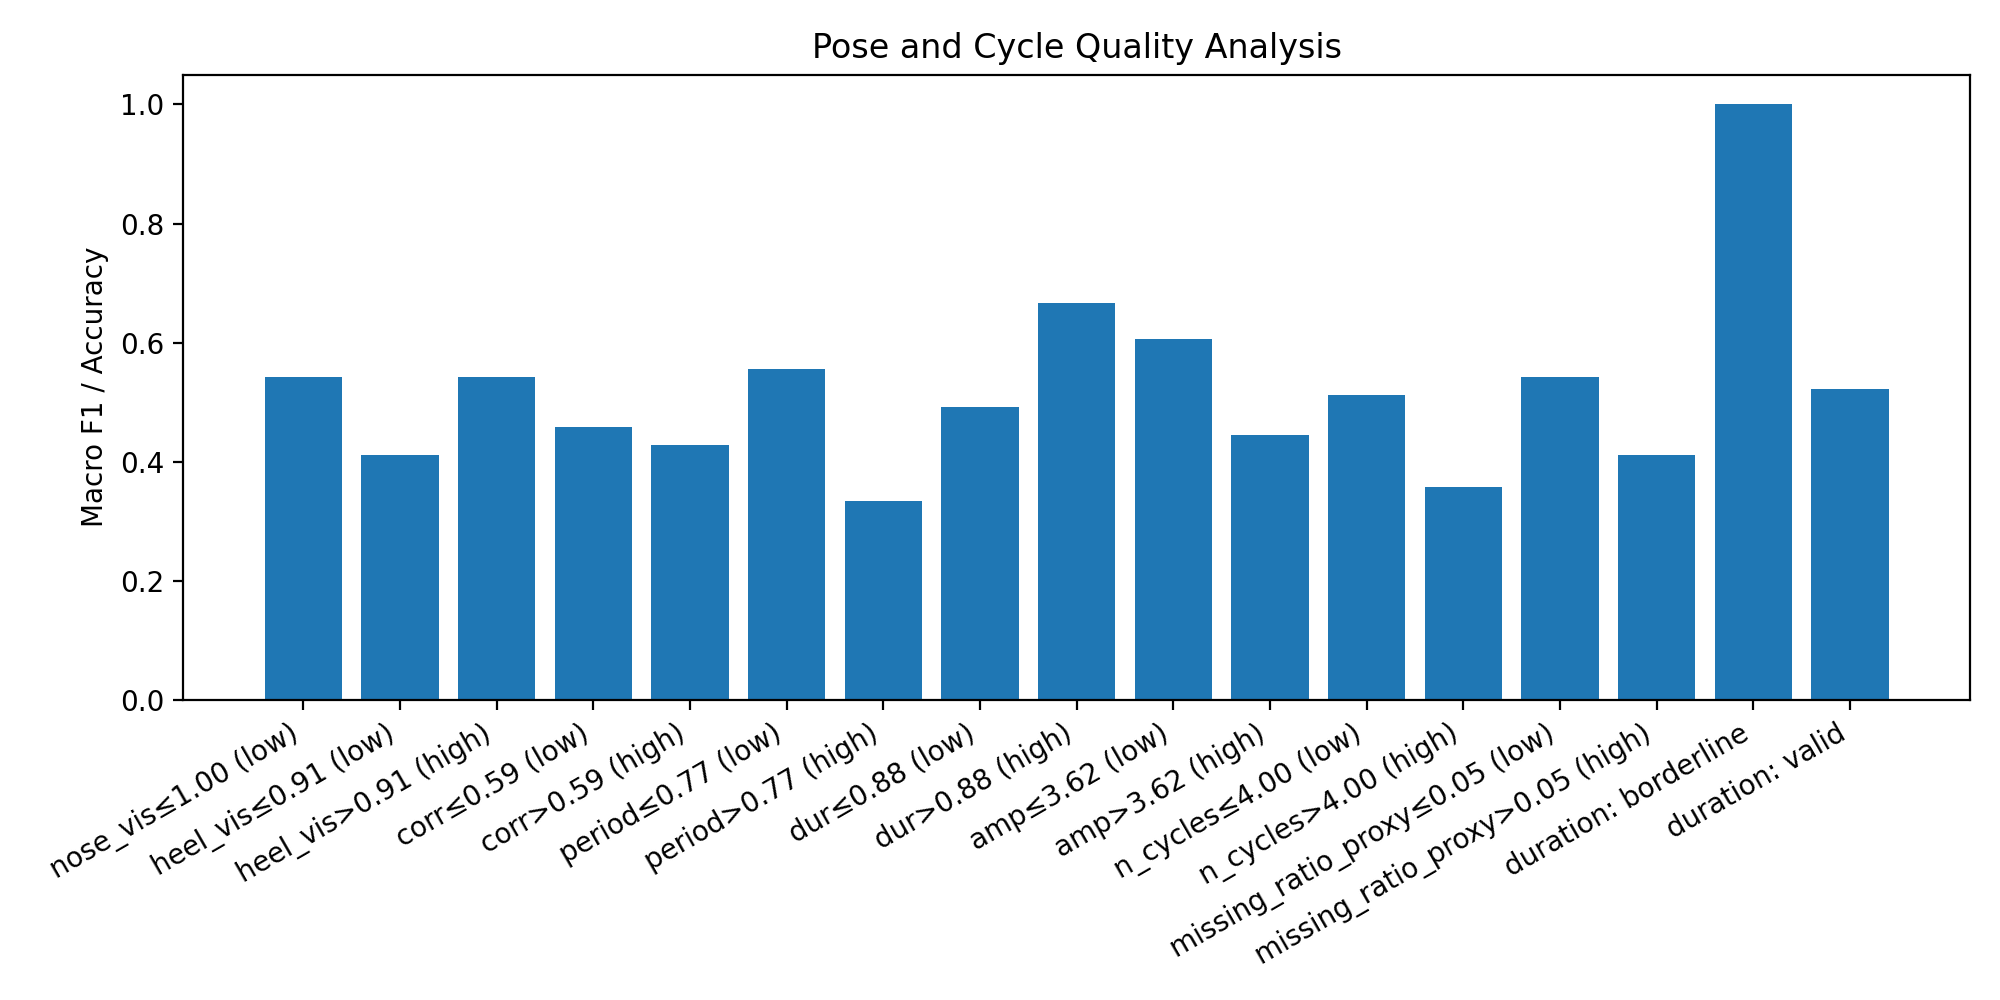
\includegraphics[width=0.85\textwidth]{figures/quality_analysis_summary.png}
\caption[Pose and cycle quality summary.]{Pose and cycle quality summary for the automatic landmark pipeline. Source: \path{quality_analysis_summary.png}.}
\label{fig:quality-analysis-summary}
\end{figure}

% ---------------------------------------------------------------------
\section{Boundary Detector and Raw Sequence Results}
\label{sec:bd-raw}

Two exploratory alternatives to rule-based cycle detection are reported here as
supplementary evidence. The learned Boundary Detector replaces autocorrelation
with a BiLSTM foot-strike detector; the raw-sequence model classifies the whole
pose sequence without explicit cycle cutting (one sample per video). Table~\ref{tab:bd-raw} summarises their best configurations.

\begin{table}[htbp]
\centering
\caption[Boundary Detector and raw-sequence pipelines.]{Boundary Detector and raw-sequence pipelines (Supplementary results). Sources: \protect\path{main_pipeline_comparison.csv}, \protect\path{bd_results.csv}, and \protect\path{raw_sequence_results.csv}.}
\label{tab:bd-raw}
\tablefont
\begin{adjustbox}{max width=\textwidth}
\begin{tabular}{llrrrr}
\toprule
Pipeline & Best config. & Test acc. & Macro-F1 & F1-false & ROC-AUC \\
\midrule
Boundary Detector & BiLSTM & 0.5000 & 0.4667 & 0.3333 & \texttt{[MISSING RESULT]} \\
Raw sequence & BiLSTM, seq$=16$, selected & 0.8333 & 0.8286 & 0.8571 & \texttt{[MISSING RESULT]} \\
\bottomrule
\end{tabular}
\end{adjustbox}
\end{table}

The Boundary Detector (best macro-F1 0.4667) does not improve on the
autocorrelation baseline and remains limited by the same scarce, noisy cycle
boundaries. The raw-sequence BiLSTM reports a high macro-F1 (0.8286), but this
figure is computed over only 12 video-level test samples and uses a different
evaluation unit (one sequence per video) than the cycle-level benchmarks; it
is therefore reported as an exploratory direction rather than as evidence that
cycle cutting is unnecessary. ROC-AUC was not stored for
either pipeline (\texttt{[MISSING RESULT]}). Both are kept out of the main
controlled comparison.

% ---------------------------------------------------------------------
\section{Summary of Main Findings}
\label{sec:summary}

Table~\ref{tab:summary} consolidates the controlled pipelines alongside the
supplementary ones. The best \emph{controlled benchmark} is bold. The
image-based row is shown without bold emphasis, in line with its exploratory
status, and the historical 76.5\% milestone of
Section~\ref{sec:version-history} is deliberately excluded from this benchmark
table.

\begin{table}[htbp]
\centering
\caption[Summary of pipeline results.]{Summary of pipeline results. The best controlled benchmark is bolded. Source: \protect\path{main_pipeline_comparison.csv}.}
\label{tab:summary}
\tablefont
\begin{adjustbox}{max width=\textwidth}
\begin{tabular}{lllrrrr}
\toprule
Pipeline & Input & Model & Acc. & Macro-F1 & F1-false & ROC-AUC \\
\midrule
\multicolumn{7}{l}{\emph{Controlled benchmark}} \\
Handmade upper bound & 13 lm $+$ vel. & CNN-BiLSTM & \textbf{0.9107} & \textbf{0.8991} & 0.8649 & 0.9556 \\
Autocorr landmark baseline & landmark feats. & MLP & 0.5455 & 0.5417 & 0.5833 & 0.6068 \\
Autocorr image-based & RGB crop & MobileNetV2$+$LSTM & 0.1111 & 0.1000 & 0.2000 & 0.0592 \\
\midrule
\multicolumn{7}{l}{\emph{Supplementary; small $N$, not controlled benchmark}} \\
Boundary Detector & landmark seq. & BiLSTM & 0.5000 & 0.4667 & 0.3333 & \texttt{[MISSING RESULT]} \\
Raw sequence & selected, seq$=16$ & BiLSTM & 0.8333 & 0.8286 & 0.8571 & \texttt{[MISSING RESULT]} \\
\bottomrule
\end{tabular}
\end{adjustbox}
\end{table}

The results give a coherent answer to the thesis research questions. First,
the markerless pose representation is sufficient to classify correct versus
false running technique when cycles are clean: the handmade upper bound reaches
0.8991 macro-F1. Second, automatic cycle detection is the dominant bottleneck:
the matched automatic baseline falls to 0.5417 macro-F1, a fixed-split gap of
0.3574. A separate 5-fold video-level CV check confirms that this is not only a
single-split artefact: handmade cycles reach $0.860 \pm 0.016$ macro-F1, while
autocorr cycles reach $0.615 \pm 0.081$, leaving a fair gap of 0.245. Together,
the ablations and robustness check attribute the loss to segmentation and pose
quality rather than to the classifier or temporal resolution. Third, within the controlled protocol
the compact landmark representation is more reliable than the RGB-crop image
representation, which collapses on this small dataset. The supplementary
boundary-detector and raw-sequence pipelines do not overturn these conclusions.
Taken together, the evidence supports investing future work in robust cycle
segmentation and pose quality rather than in larger classifiers or richer image
representations. Consistent with this scope, the results do
not claim real-world deployment readiness.
% =====================================================================
% chapters/06_discussion.tex
% Chapter 6 — Discussion
% Project: Vision-Based Running Technique Classification from In-the-Wild
%          Internet Videos using Markerless Pose Estimation and Deep Learning
%
% This chapter interprets the results reported in Chapter 5; it does not
% re-tabulate them. Numerical values are quoted only where needed to anchor
% an interpretation, and refer back to the controlled tables of Chapter 5.
% Controlled benchmark results and historical development results are kept
% strictly separate. No claim of real-world deployment readiness is made.
% =====================================================================

\chapter{Discussion}
\label{ch:discussion}

This chapter interprets the empirical results of Chapter~\ref{ch:results}. The
guiding question is not only \emph{how well} the pipelines perform, but
\emph{where} performance is gained and lost, and \emph{what that implies} for
the dataset and protocol used in this work.

% ---------------------------------------------------------------------
\section{Interpretation of the Main Findings}
\label{sec:disc-main}

The central pattern across all experiments is a decoupling between
\emph{representation learnability} and \emph{automatic segmentation
reliability}. When running cycles are correctly segmented, the markerless pose
representation is clearly sufficient: the handmade upper bound separates
correct from false technique at a macro-F1 near 0.90
(Section~\ref{sec:handmade}) . When the same representation and classifiers are
driven by automatically detected cycles, performance falls to roughly chance
(Section~\ref{sec:autocorr-baseline}) . The natural reading is that the
classification \emph{model} is not the binding constraint; the binding
constraint is the upstream pipeline that converts raw, uncontrolled video into
clean, comparable cycle samples.

This conclusion is supported at two levels. The fixed-split benchmark shows a
drop from 0.8991 macro-F1 for handmade cycles to 0.5417 for the autocorr
baseline. The fair-gap robustness check then repeats the comparison with the
same MLP classifier under 5-fold video-level cross-validation: handmade cycles
reach $0.860 \pm 0.016$ macro-F1, while autocorr cycles reach
$0.615 \pm 0.081$, leaving a fair gap of 0.245. Thus, the loss is not only a
single-split artefact; it remains visible when the comparison is repeated across
video-level folds.

This interpretation reframes the contribution of the thesis. The work does not
claim a high-accuracy automatic classifier. Instead, it provides evidence,
through a matched upper-bound/baseline design and a series of ablations, that
the difficulty of in-the-wild running-technique analysis lies predominantly in
robust cycle detection and pose quality rather than in the choice of classifier
or representation depth. Every subsequent section in this chapter can be read
as locating one facet of that bottleneck.

% ---------------------------------------------------------------------
\section{Effect of Cycle Source}
\label{sec:disc-cycle-source}

The comparison between the handmade and autocorrelation (autocorr) pipelines
(Section~\ref{sec:hm-vs-ac}) is the most informative single contrast in the
study. Because the two pipelines share the landmark representation, classifier
family, split, and reporting protocol, the large gap between them isolates the
effect of cycle segmentation almost cleanly: the manual and automatic pipelines
differ chiefly in \emph{how cycle boundaries are obtained}. The fair-gap
robustness check strengthens this interpretation: under the same MLP classifier
and 5-fold video-level cross-validation, handmade cycles achieve
$0.860 \pm 0.016$ macro-F1, whereas autocorr cycles achieve
$0.615 \pm 0.081$. The 0.245 macro-F1 fair gap shows that the fixed-split
drop is not simply due to one unlucky train/test partition.

Two mechanisms plausibly explain the gap. First, automatic detection discards a
substantial fraction of the data: many videos yield no usable cycle at all, and
of those that do, a large share of raw cycles are rejected by the
duration/quality filters (Section~\ref{sec:signal-ablation}). The surviving
cycles are therefore both fewer and biased toward easier cases. Second, even
retained cycles may have imprecise foot-strike-to-foot-strike boundaries, so
that the eight-phase samples are not temporally aligned across examples. A
classifier that performed well on manually aligned phases then faces a
distribution of misaligned, partially mis-segmented inputs. 

The validation-to-test collapse of the sequential models under automatic cycles
(Section~\ref{sec:autocorr-baseline}) is consistent with this misalignment: the
models latch onto regularities that do not transfer once boundaries vary. The
practical message is that improving the automatic pipeline should target
detection coverage and boundary precision before any change to the classifier.

The permutation test further tempers the interpretation of the autocorr signal.
The observed autocorr MLP CV macro-F1 was 0.5206, compared with a permutation
null mean of 0.468 and $p = 0.2475$. This does not prove that the automatic
features contain no information; rather, it suggests that the information is
weak and unstable under a simple MLP configuration. This is consistent with a
pipeline whose errors originate upstream in cycle boundary quality.

% ---------------------------------------------------------------------
\section{Effect of Representation: Landmark versus Image}
\label{sec:disc-representation}

On a matched automatic cycle source, the landmark representation clearly
outperformed the RGB-crop image representation
(Section~\ref{sec:representation}), and the image pipeline collapsed below
chance in the controlled rerun (Section~\ref{sec:image-results}). At first
sight this is surprising, since RGB crops carry strictly more raw information
(silhouette, limb contour, clothing-relative motion) than sparse landmarks.

The likely explanation is not that this information is useless, but that the
image pipeline cannot exploit it reliably under the present conditions: a small
training set, a high-capacity visual backbone prone to overfitting, and crop
instability driven by the same noisy pose estimates that bound the boundary
quality. In effect, the image pipeline inherits the segmentation bottleneck and
adds a second source of variance --- the runner-centred crop --- on top of it.

The landmark representation, by contrast, acts as a compact inductive bias:
by reducing each frame to a fixed set of joint coordinates, it discards
appearance variation that would otherwise have to be learned away from limited
data. For this dataset, that compression is an advantage rather than a loss.
The appropriate conclusion is conditional: image-based modelling is not
invalidated in principle, but the current implementation is not yet stable
enough to compete with the landmark baseline. A fair re-test would require more
data and more robust cropping.

This is also the right place to interpret the historical
\texttt{autocorr\_fixed} (val\_acc 76.5) milestone
(Section~\ref{sec:version-history}) . It represents the most technically ambitious
step in the project's development --- the move from landmark-only sequences to
an image-based MobileNetV2--LSTM pipeline --- and it motivated the organised
image-based rerun. However, its 76.5\% figure is a historical validation
accuracy from a development notebook, recorded under a different protocol and
never re-confirmed on the fixed test split. The controlled rerun did not
reproduce it. The milestone is therefore valuable as evidence of methodological
exploration and as the reason the image direction was worth testing, but it
cannot serve as a benchmark and must not be compared directly against the
controlled landmark baseline.

% ---------------------------------------------------------------------
\section{Effect of Model Architecture}
\label{sec:disc-model}

The model ablation (Section~\ref{sec:model-ablation}) shows that architecture
matters far less than data quality. On the clean handmade data, the CNN-BiLSTM
achieved the strongest macro-F1, while the 1D-CNN, BiLSTM, and MLP remained
close enough to show that the spread across architectures was narrow. This
indicates that, given well-segmented cycles, the discriminative signal is
accessible to several standard architectures and does not depend solely on deep
temporal machinery.

On the automatic pipeline the more expressive sequential models behaved
unstably. The 1D-CNN and BiLSTM both produced zero F1 for the false class at
their operating thresholds, while the CNN-BiLSTM looked best at the default
0.5 threshold but became unstable under validation-tuned thresholding. High-capacity sequence models
are precisely those most able to overfit the spurious regularities introduced
by inconsistent segmentation, so their poor generalisation is symptomatic of
the upstream noise rather than of an architectural deficiency. The robustness
of the simple MLP as the reported automatic baseline follows from the same
logic: with noisy, scarce inputs, a lower-variance model is preferable. This
argues against reaching for larger classifiers as a remedy for the automatic
pipeline's weakness.

% ---------------------------------------------------------------------
\section{Effect of Signal Choice}
\label{sec:disc-signal}

The signal ablation (Section~\ref{sec:signal-ablation}) exposed a tension
between two notions of a ``good'' detection signal. The vertical-oscillation
signals (\texttt{head\_y}, \texttt{hip\_y}) detected cycles in more videos and,
for \texttt{hip\_y}, even produced the highest downstream classification
macro-F1. Yet they admitted many ill-formed cycles, reflected in weak mean
autocorrelation and a large number of duration-based rejections.

The \texttt{contact\_diff} signal showed a different profile: fewer detected
videos, but cycle boundaries that were more directly tied to foot-contact
events and therefore more suitable for foot-strike-to-foot-strike sampling.
Selecting \texttt{contact\_diff} as the baseline signal therefore reflects a
deliberate preference for boundary \emph{precision} over detection
\emph{coverage}. This is the defensible choice for a pipeline whose downstream
representation is an eight-phase sampling that assumes accurate
foot-strike-to-foot-strike boundaries: a cleanly segmented minority is more
useful than a larger but temporally inconsistent set. 

The fact that \texttt{hip\_y} scored a higher macro-F1 is interpreted cautiously, given the
small test set and the risk that more permissive detection coincided with
easier videos rather than with genuinely better segmentation. The broader
lesson is that signal selection for in-the-wild data must be judged on
segmentation quality, not only on a single end-to-end accuracy number.

% ---------------------------------------------------------------------
\section{Effect of Feature Representation}
\label{sec:disc-feature}

The feature ablation (Section~\ref{sec:feature-ablation}) found that the
selected 13-landmark representation and the selected-landmark-plus-velocity
variant matched the best handmade macro-F1, while the full 33-landmark and
lower-body-only variants remained close but did not improve the overall
macro-F1. The conservative interpretation is that additional landmarks may
carry complementary cues for one class, but they did not produce a more robust
overall result on this split.

The near-equivalence of the selected-landmark
configurations supports using the compact representation as the pipeline
default, especially for the automatic experiments where every additional input
dimension also imports additional pose-estimation noise. This connects back to the representation discussion
(Section~\ref{sec:disc-representation}): both results favour parsimony.
Reducing the input to a small, well-chosen set of joints limits the model's
exposure to noise and to spurious appearance variation, which is advantageous
precisely because the dataset is small and the upstream estimates are imperfect.
The choice of features should therefore be coupled to the data regime rather
than maximised in isolation.

% ---------------------------------------------------------------------
\section{Effect of Frame Resolution per Cycle}
\label{sec:disc-frames}

The frames-per-cycle ablation (Section~\ref{sec:frames-ablation}) showed no
benefit from increasing temporal resolution beyond the eight-phase
representation, and there was no monotonic trend across frame counts. The
eight-phase sampling remained the strongest and most compact setting. The
interpretation is that eight phases already capture the salient kinematic
structure of a running cycle for this binary task; finer sampling mostly adds
redundant frames and, on limited data, additional opportunity to overfit rather
than additional discriminative signal.

This finding has a useful methodological consequence: the eight-phase
representation is justified not merely by convention but by an explicit
cost-benefit comparison. It keeps sample dimensionality low, which is
consistent with the parsimony favoured by the model and feature analyses, and
it reduces the computational burden of the pipeline without a meaningful
accuracy penalty.

% ---------------------------------------------------------------------
\section{Cycle-Level versus Video-Level Interpretation}
\label{sec:disc-cycle-video}

Aggregating cycle predictions to the video level by majority vote consistently
improved the automatic baseline (Section~\ref{sec:cycle-vs-video}), and the same
direction held for the other pipelines. This is the expected behaviour when
per-cycle predictions contain independent noise: aggregating several cycles from
the same video lets correct predictions outweigh sporadic errors, reducing
variance. Because the underlying data unit is the video, not the cycle,
video-level reporting is also the more faithful measure of practical
performance and is therefore the appropriate headline metric for any future
deployment-oriented evaluation.

The interpretation must nonetheless be tempered by sample size. The video-level
evaluation rests on only a handful of test videos, several of which contribute a
single cycle. The improvement from aggregation is consistent and theoretically
motivated, but its precise magnitude is uncertain at this scale, and the result
should be read as directional evidence rather than as a calibrated estimate.

% ---------------------------------------------------------------------
\section{Effect of Threshold Selection}
\label{sec:disc-threshold}

The threshold analysis (Section~\ref{sec:threshold}) revealed an asymmetry
between the clean and the automatic pipelines. On the handmade data,
validation-selected thresholds were mostly neutral or beneficial. On the
automatic data, the same procedure left the robust MLP unchanged but sharply
degraded the sequential models, with the CNN-BiLSTM losing substantial macro-F1
and being flagged as threshold-overfit.

This is the resolution of the apparent
contradiction with the model ablation: the CNN-BiLSTM looks best at the default
threshold but is unstable once a validation-chosen threshold is applied to
test, whereas the MLP is stable, which is why it is the reported baseline.
The deeper interpretation is that decision-threshold tuning is only as reliable
as the validation set on which it is performed. With a small validation split
and noisy automatic cycles, the validation-optimal threshold need not transfer,
and tuning can transfer noise rather than signal. 

The methodological
implication, reflected in the reporting throughout Chapter~\ref{ch:results}, is
that any tuned result must state that the threshold was selected on validation
and must be accompanied by the default-threshold result, so that threshold
overfitting is visible rather than hidden.

% ---------------------------------------------------------------------
\section{Effect of Pose and Cycle Quality}
\label{sec:disc-quality}

The quality analysis (Section~\ref{sec:quality}) provides the most direct
evidence for the segmentation-bottleneck interpretation. Classification
accuracy on the automatic pipeline rose with higher heel visibility, lower
landmark missing-ratio, and stronger autocorrelation of the cycle signal. In
other words, the errors are not distributed uniformly across the test set; they
concentrate in cycles where pose estimation is unreliable or the periodic
structure is weak.

Together with the failed-video breakdown, which attributes
the majority of failures to the cycle-detection stage, this locates the
dominant error source firmly upstream of the classifier. This is the unifying thread of the discussion. The cycle-source gap
(Section~\ref{sec:disc-cycle-source}), the fragility of expressive models under
automatic cycles (Section~\ref{sec:disc-model}), the preference for the
boundary-precise \texttt{contact\_diff} signal
(Section~\ref{sec:disc-signal}), and the instability of the image pipeline
(Section~\ref{sec:disc-representation}) are all consequences of the same
underlying limitation: imperfect markerless pose estimation and the difficulty
of detecting clean running cycles in uncontrolled footage. The quality analysis
makes that limitation measurable.

% ---------------------------------------------------------------------
\section{Error Analysis}
\label{sec:disc-error}

Synthesising the error evidence, three failure modes can be distinguished. First, \emph{detection failures}: videos in which no usable cycle is found, so
the system cannot make a prediction at all; these dominate the failed-video
counts and arise mainly at the cycle-detection stage
(Section~\ref{sec:quality}) . Second, \emph{segmentation errors}: cycles that are
detected but poorly bounded, producing misaligned eight-phase samples that
degrade classification even when pose visibility is adequate; the
validation-to-test collapse of the sequential models is the clearest symptom
(Section~\ref{sec:autocorr-baseline}) . Third, \emph{classifier errors} on
genuinely clean cycles, which the handmade results show to be comparatively
rare.

The relative weight of these modes is itself a result: the first two,
both upstream, account for the bulk of the gap between the upper bound and the
automatic baseline, while the third is small. This ordering should guide
remediation. Reducing detection and segmentation errors --- through more robust
pose estimation, better signal conditioning, or a learned boundary detector
trained on more data --- is likely to yield far larger gains than further work
on the classifier. The exploratory boundary-detector and raw-sequence pipelines
(Section~\ref{sec:bd-raw}) are first steps in that direction, but on the present
data they did not yet improve over the rule-based baseline and remain
inconclusive.

% ---------------------------------------------------------------------
\section{Limitations}
\label{sec:disc-limitations}

Several limitations bound the conclusions of this work. The dataset is small,
and the validation and test splits in particular are very small
(Section~\ref{sec:dataset-stats}) ; consequently, single-point differences,
figures after threshold tuning, and the highest-scoring feature configuration
should be treated as indicative rather than precise. The 5-fold fair-gap check
partly mitigates this concern by repeating the main handmade--autocorr contrast
across folds, but it does not remove the need for a larger external dataset. The video-level results
also rest on few videos. The class distribution is moderately imbalanced at the
video level, which is mitigated but not eliminated by the use of macro-F1
\cite{sokolova2009metrics}.

The pipeline also inherits the limitations of its components. Markerless pose
estimation is itself noisy on in-the-wild footage \cite{bazarevsky2020blazepose}.
Recent markerless-running analyses also note that such noise can affect
downstream biomechanical interpretation \cite{panconi2024markerless}. In this
pipeline, that noise propagates into signal extraction, cycle detection, and
--- for the image pipeline --- crop stability. 

Cycle detection relies on a
periodicity assumption that does not hold for very short clips or atypical gait,
contributing to detection failures. The handmade pipeline, used as the upper
bound, depends on manual segmentation and therefore reflects an idealised
condition that an automatic system cannot fully attain. Finally, all results
are obtained on a single corpus collected under one labelling convention;
generalisation to other populations, camera viewpoints, and definitions of
``correct'' technique remains untested. The historical version-history results
(Section~\ref{sec:version-history}) are excluded from all benchmark claims for
the reasons given above and add a further caution against over-reading
development-stage numbers. The permutation test is also limited by the same
small autocorr sample size and should be interpreted as a diagnostic robustness
check, not as a definitive statistical claim about all possible classifiers.

% ---------------------------------------------------------------------
\section{Practical Implications}
\label{sec:disc-practical}

The practical implications follow directly from the bottleneck analysis. For
researchers and practitioners building on this work, effort is best invested in
the upstream stages: more robust markerless pose estimation, signal conditioning
that improves cycle-boundary precision, and data-driven boundary detection
trained on enough examples to outperform rule-based autocorrelation. The
evidence indicates that such improvements would raise the automatic pipeline
toward the handmade upper bound more effectively than any change to the
classifier or any increase in temporal or feature resolution. Where an
automatic system is used, predictions should be reported and consumed at the
video level, with explicit handling of videos for which no reliable cycle can
be detected.

It must be stated plainly that these results do not establish deployment
readiness. The automatic pipeline performs near chance on the controlled test
set, the evaluation rests on a small single-source dataset, and the upper bound
depends on manual segmentation that a deployed system would not have. 

The
appropriate framing of the contribution is diagnostic: the work demonstrates
that markerless pose sequences can encode running-technique distinctions when
cycles are clean, and it identifies, through controlled comparison and
ablation, exactly where an automatic in-the-wild system currently breaks down.
Turning that diagnosis into a usable tool is left to future work
(Chapter~\ref{ch:conclusion}) .

% End of Chapter 6
% =====================================================================
% chapters/07_conclusion.tex
% Chapter 7 — Conclusion and Future Work
% Project: Vision-Based Running Technique Classification from In-the-Wild
%          Internet Videos using Markerless Pose Estimation and Deep Learning
%
% Headline metrics quoted below are the controlled results established in
% Chapter 5; they are not re-derived here. No claim of clinical,
% professional, or real-world deployment readiness is made.
% =====================================================================

\chapter{Conclusion and Future Work}
\label{ch:conclusion}

% ---------------------------------------------------------------------
\section{Conclusion}
\label{sec:concl-summary}

This thesis addressed the problem of classifying running technique as correct or
false from \emph{in-the-wild} internet videos using markerless pose estimation
and deep learning. The work developed a complete pipeline consisting of
markerless pose estimation, landmark filtering and normalisation, motion-signal
extraction, running-cycle detection, eight-phase sampling, landmark-based or
image-based cycle representation, deep-learning classification, and evaluation
under a fixed split by video identifier.

The experimental design separated two questions that are often mixed together:
whether the pose representation is learnable when cycle boundaries are reliable,
and how much performance is lost when cycle boundaries must be detected
automatically. The handmade landmark pipeline, using controlled cycle
segmentation, reached a test accuracy of 0.9107 and a macro-F1 of 0.8991. This
result is interpreted as an upper bound, not as a deployment baseline. The
autocorrelation-based landmark pipeline, using automatic cycles detected from
the \texttt{contact\_diff} signal, reached a test accuracy of 0.5455 and a
macro-F1 of 0.5417 under the reported baseline setting. Because the two
pipelines use the same general pose-representation family but differ in cycle
source, the gap between them localises the main difficulty of the task in the
automatic cycle-detection stage. This interpretation is supported by an
additional fair-gap robustness check: under the same MLP classifier and
5-fold video-level cross-validation, handmade cycles achieved
$0.860 \pm 0.016$ macro-F1, whereas autocorr cycles achieved
$0.615 \pm 0.081$, giving a fair gap of 0.245 macro-F1. A 100-permutation test
on the autocorr MLP setting did not reach statistical significance
($p = 0.2475$), suggesting that the autocorr-derived features are not yet
robustly separable under that simple classifier.

The ablation studies and extended analyses refine this conclusion. The model
ablation showed that architecture choice matters less than segmentation quality:
the CNN-BiLSTM is strongest on clean handmade cycles, while the simpler MLP is
more stable as the reported automatic baseline after validation-based threshold
selection. The feature ablation showed that compact selected-landmark
representations are sufficient and competitive with larger landmark sets. The
frames-per-cycle ablation showed that eight-phase sampling is an efficient
choice, since increasing the number of sampled frames did not improve macro-F1.

The signal ablation showed a trade-off between detection coverage and
semantically meaningful foot-strike-to-foot-strike boundaries; \texttt{contact\_diff}
was therefore retained as the main baseline signal even though \texttt{hip\_y}
achieved the highest classification macro-F1 in the signal ablation. The
controlled landmark-versus-image comparison showed that the RGB-crop
MobileNetV2--LSTM pipeline did not reproduce the historical image-based
development result and was not stable enough to replace the landmark baseline.

Taken together, the results support a diagnostic conclusion. Markerless pose
sequences can encode correct-versus-false running-technique differences when
cycles are clean, but the current automatic pipeline is limited by pose quality,
cycle detection, and boundary alignment. The fixed-split result and the
cross-validation robustness check point to the same conclusion, while the
permutation test shows that the autocorr representation remains statistically
fragile under a simple MLP. The thesis therefore does not claim
real-world deployment readiness. Its contribution is to identify where the
automatic in-the-wild pipeline succeeds, where it fails, and which components
should be improved before any practical feedback system is attempted.

% ---------------------------------------------------------------------
\section{Answers to Research Questions}
\label{sec:concl-rqs}

The seven research questions introduced in Section~\ref{sec:intro-rqs} are
answered below using the controlled results from Chapter~\ref{ch:results}.

\paragraph{RQ1 --- Can pose-based classifiers distinguish correct from false
technique under reliable segmentation?}
Yes. Under reliable manually controlled cycle segmentation, the handmade
landmark upper bound reached a test accuracy of 0.9107 and a macro-F1 of
0.8991. All handmade models exceeded 0.85 macro-F1, and the best CNN-BiLSTM
model reached the strongest overall result. This shows that the markerless pose
representation contains useful information for distinguishing correct from
false running technique when the running cycles are cleanly segmented.

\paragraph{RQ2 --- How much performance is lost when handmade cycles are
replaced by automatic autocorrelation-based detection?}
The loss is substantial. On the controlled fixed split, the reported autocorr
landmark baseline reached a test accuracy of 0.5455 and a macro-F1 of 0.5417,
compared with 0.9107 accuracy and 0.8991 macro-F1 for the handmade upper
bound. This corresponds to a drop of 0.3652 in accuracy and 0.3574 in
macro-F1. The fair 5-fold video-level CV check confirms that this loss is not
only a fixed-split artefact: under the same MLP classifier and threshold 0.5,
handmade cycles reached $0.860 \pm 0.016$ macro-F1, while autocorr cycles
reached $0.615 \pm 0.081$, leaving a fair gap of 0.245 macro-F1. A permutation
test on the autocorr MLP setting did not reach statistical significance
($p = 0.2475$), suggesting that autocorr-derived features are not yet robustly
separable under this simple classifier. Since the comparison keeps the general
landmark-representation family fixed while changing the cycle source, the loss
is attributed primarily to automatic cycle detection and boundary alignment.

\paragraph{RQ3 --- Which motion signal is most reliable for automatic cycle
detection?}
The answer depends on the criterion. In the signal ablation, \texttt{hip\_y}
achieved the highest downstream classification macro-F1 (0.7321) and accuracy
(0.7333). However, \texttt{contact\_diff} was retained as the main automatic
baseline signal because it is more directly tied to foot-contact dynamics and
supports foot-strike-to-foot-strike cycle interpretation. Thus, \texttt{hip\_y}
was the strongest signal by classification score in this ablation, while
\texttt{contact\_diff} was the most appropriate baseline signal for
semantically aligned cycle detection.

\paragraph{RQ4 --- Which architecture is most suitable for eight-phase pose
sequences?}
The answer is pipeline-dependent. On the handmade upper-bound pipeline, the
CNN-BiLSTM achieved the best macro-F1 (0.8991), indicating that local temporal
patterns and sequential modelling are useful when cycle alignment is reliable.
On the automatic autocorr pipeline, the CNN-BiLSTM was strongest at the default
0.5 threshold, but it became unstable under validation-tuned thresholding. The
MLP was therefore used as the more robust reported automatic baseline. This
suggests that higher model capacity is useful only when the cycle samples are
reliable; it does not compensate for noisy automatic segmentation.

\paragraph{RQ5 --- How do feature representation and frames-per-cycle affect
performance?}
The selected 13-landmark representation and the selected-landmark-plus-velocity
variant matched the best handmade macro-F1 (0.8991), while the full
33-landmark and lower-body-only variants remained close but did not improve the
overall macro-F1. This supports using a compact landmark representation as the
default. For temporal resolution, the eight-frame setting achieved the best
macro-F1 (0.8991), while 16, 24, and 32 frames did not yield a monotonic
improvement. The eight-phase representation is therefore both effective and
computationally economical for this dataset.

\paragraph{RQ6 --- How does the image-based representation compare with the
landmark-based representation under the autocorr pipeline?}
Under the controlled matched-cycle comparison, the landmark representation was
clearly more reliable. The autocorr landmark baseline reached a macro-F1 of
0.5417, while the image-based MobileNetV2--LSTM pipeline reached only 0.1000
macro-F1 and a ROC-AUC of 0.0592. The historical
\texttt{autocorr\_fixed} image-based milestone with validation accuracy 76.5\%
was not reproduced under the final fixed-split protocol. It is therefore treated
as development evidence and motivation for the organised image-based rerun, not
as a benchmark result.

\paragraph{RQ7 --- How do cycle aggregation, threshold selection, and pose/cycle
quality affect interpretation?}
Each factor materially affects interpretation. Aggregating cycle-level
predictions to the video level by majority vote improved the automatic landmark
baseline from 0.5139 to 0.5333 macro-F1, although the video-level test set was
small. Validation-tuned thresholds improved or preserved some clean handmade
results but overfit several automatic-pipeline models, especially the
CNN-BiLSTM. The quality analysis showed that higher heel visibility, lower
missing-ratio, and stronger autocorrelation were associated with better
classification accuracy. These findings confirm that evaluation should report
cycle-level and video-level behaviour, state whether thresholds are tuned on
validation, and account for pose and cycle quality.

% ---------------------------------------------------------------------
\section{Future Work}
\label{sec:concl-future}

The findings point to several future directions, ordered by their likely impact
on the automatic pipeline.

\begin{itemize}
    \item \textbf{Larger and more diverse dataset.} The validation and test sets
    are small, so future work should collect more in-the-wild videos across
    more runners, camera viewpoints, running speeds, clothing conditions,
    and recording environments.
    
    \item \textbf{Stronger foot-strike and cycle-boundary annotation.} Since the
    largest performance gap comes from replacing handmade cycles with
    automatic cycles, higher-quality foot-strike annotations should be
    collected to train and evaluate better boundary detectors.
    
    \item \textbf{Improved automatic cycle detection.} The current
    autocorrelation approach is interpretable but limited. Future work
    should compare it with learned boundary detectors, temporal
    segmentation models, and hybrid methods that combine periodicity,
    foot-contact cues, and confidence-based filtering.
    
    \item \textbf{Pose-quality-aware filtering and weighting.} The quality
    analysis indicates that errors concentrate in low-visibility or weakly
    periodic cycles. Future systems should explicitly use pose visibility,
    landmark missing-ratio, autocorrelation strength, and cycle-quality
    scores to reject, weight, or calibrate predictions.
    
    \item \textbf{Expert biomechanics validation.} The correct/false labels and
    recovered kinematic patterns should be checked against expert assessment
    so that the classification target is better grounded in running-form
    criteria.
    
    \item \textbf{More robust image-based modelling.} The controlled image rerun
    showed that RGB crops are unstable in the current implementation.
    Future work should improve runner tracking, bounding-box smoothing,
    crop stabilisation, and data augmentation before drawing conclusions
    about the value of image-based representations.
    
    \item \textbf{Pose--image fusion.} Rather than choosing between landmarks and
    crops, future models could fuse a compact landmark stream with a
    stabilised visual stream, combining the robustness of pose coordinates
    with visual cues such as silhouette and limb contour.
    
    \item \textbf{Video-level decision protocol.} Since aggregation can reduce
    cycle-level noise, future work should treat video-level prediction as a
    first-class evaluation target, compare majority vote with probability
    averaging and confidence voting, and report uncertainty when few cycles
    are available.
    
    \item \textbf{Deployment only after validation.} A real-time coaching or
    feedback tool is a possible long-term direction, but it should only be
    considered after the automatic pipeline is validated on larger,
    representative data and shown to be reliable across viewpoints and
    runner populations.
\end{itemize}

The final conclusion is therefore deliberately conservative. This thesis shows
that markerless pose data from in-the-wild running videos can support
running-technique classification when cycle segmentation is reliable. It also
shows that the current automatic system is limited mainly by upstream pose and
cycle quality. The next stage of work should therefore prioritise robust cycle
detection, larger validation data, and expert-labelled evaluation before moving
toward practical deployment.

% End of Chapter 7

% -------------------- Appendices --------------------
\clearpage
\appendix % Reset bộ đếm chương sang định dạng chữ cái (Appendix A, Appendix B,...)
% =====================================================================
% appendices/appendix_a_implementation.tex
% Appendix A — Implementation Details
% Project: Vision-Based Running Technique Classification from In-the-Wild
%          Internet Videos using Markerless Pose Estimation and Deep Learning
%
% Required preamble packages in main.tex:
%   \usepackage{booktabs}
%   \usepackage{array}
%   \usepackage{tabularx}
%   \usepackage{graphicx}
%
% This appendix documents implementation only. Configuration values are
% reported only when available from the project notebooks, exported reports,
% or experiment inventory. Missing training hyper-parameters are explicitly
% marked as not exported rather than inferred.
% =====================================================================

\chapter{Implementation Details}
\label{app:implementation}

This appendix documents the implementation behind the experiments of
Chapters~\ref{ch:experimental-setup}--\ref{ch:results}: the notebook
organisation, the output directory layout, the files each stage produces, and
the configuration settings. It is provided for reproducibility; no additional
result claims are introduced here. Configuration values are reported only when
they are available from the project notebooks or exported reports; values that
were not exported are explicitly marked as unavailable rather than inferred.

% ---------------------------------------------------------------------
\section{Notebook Mapping}
\label{app:notebook-mapping}

The pipeline is implemented as a sequence of self-contained notebooks.
Table~\ref{tab:notebook-mapping} maps each notebook to the pipeline stage it
realises and the principal role it plays in the thesis. Notebooks numbered with
a letter suffix (03b--03g) are extended or supplementary analyses; the others
are core pipeline stages.

\begin{table}[htbp]
\centering
\caption{Mapping of project notebooks to pipeline stages and thesis roles.}
\label{tab:notebook-mapping}
\renewcommand{\arraystretch}{1.18}
\scriptsize
\begin{tabularx}{\textwidth}{
>{\raggedright\arraybackslash}p{0.08\textwidth}
>{\raggedright\arraybackslash}p{0.34\textwidth}
>{\raggedright\arraybackslash}X
>{\raggedright\arraybackslash}p{0.16\textwidth}}
\toprule
ID & Notebook & Purpose & Role \\
\midrule
00  & \path{00_dataset_split_and_eda} & Dataset construction, video-level splitting, and exploratory data analysis. & Core \\
01  & \path{01_handmade_8frame_upper_bound} & Handmade eight-phase cycle pipeline used as the controlled upper-bound reference. & Core \\
02  & \path{02_autocorr_cycle_detection_baseline} & Automatic autocorrelation-based landmark baseline using motion signals and detected cycles. & Core \\
03  & \path{03_handmade_vs_autocorr_comparison} & Comparison between manually controlled cycle segmentation and automatic cycle detection. & Core \\
03b & \path{03b_autocorr_image_based_pipeline} & Image-based autocorr pipeline using runner crops and a MobileNetV2--LSTM classifier. & Supplementary \\
03c & \path{03c_autocorr_version_comparison} & Autocorr version history and method-evolution summary. & Supplementary \\
03d & \path{03d_representation_comparison_landmark_vs_image} & Landmark-only versus image-based representation comparison. & Supplementary \\
03e & \path{03e_cycle_level_vs_video_level_evaluation} & Cycle-level and video-level evaluation with aggregation. & Supplementary \\
03f & \path{03f_pose_cycle_quality_analysis} & Pose-quality and cycle-quality analysis for interpreting failures. & Supplementary \\
03g & \path{03g_threshold_05_vs_tuned_report} & Comparison between default threshold 0.5 and validation-tuned threshold. & Supplementary \\
03h & \path{03h_autocorr_cv_robustness_check} & Fair handmade--autocorr gap under 5-fold video-level CV and autocorr MLP permutation test. & Core support \\
04  & \path{04_model_ablation} & Architecture ablation over MLP, 1D-CNN, BiLSTM, and CNN-BiLSTM. & Core \\
05  & \path{05_feature_ablation} & Input feature-set comparison. & Core \\
06  & \path{06_signal_ablation_cycle_detection} & Comparison of motion signals for cycle detection. & Core \\
07  & \path{07_frames_per_cycle_ablation} & Comparison of 8, 16, 24, and 32 sampled frames per cycle. & Core \\
08  & \path{08_boundary_detector_pipeline} & Learned boundary-detection pipeline. & Supplementary \\
09  & \path{09_raw_sequence_bilstm_gru} & Raw-sequence BiLSTM/GRU pipeline without fixed eight-phase sampling. & Supplementary \\
10  & \path{10_threshold_tuning_and_calibration} & Threshold sweep and calibration analysis. & Supplementary \\
11  & \path{11_error_analysis} & Error analysis used to support the discussion of failure modes. & Core support \\
12  & \path{12_final_report_tables_and_figures} & Core report tables and figures. & Core \\
12b & \path{12b_extended_final_report_tables} & Extended report tables and final summary figures. & Supplementary \\
\bottomrule
\end{tabularx}
\end{table}

% ---------------------------------------------------------------------
\section{Directory Structure}
\label{app:directory}

All notebooks write to a fixed output directory under a configurable
\texttt{DRIVE\_BASE} root, so that downstream aggregation notebooks can locate
artefacts regardless of where the project is mounted. The principal layout is
shown below.

\lstset{
  breaklines=true,      % Tự động ngắt dòng khi chạm lề
  basicstyle=\ttfamily\small, % Phông chữ máy tính nhỏ gọn gọn gàng
  columns=flexible,
  keepspaces=true
}

\begin{lstlisting}
DRIVE_BASE/
  outputs/
    dataset/          # split lists, split_summary, metadata
    eda/              # class/duration/fps/frame distributions, split charts
    handmade/         # handmade results, predictions, reports, curves, *.pth
    autocorr/         # autocorr results, cycle stats, fair-gap CV/permutation files
    autocorr_image/   # image results, cycle stats, crops, reports, *.pth
    ablation/         # model / feature / signal / frames ablation CSVs
    reports/          # comparison CSVs/MD, extended summaries, figures
    figures/          # copied thesis-ready figures
\end{lstlisting}

% ---------------------------------------------------------------------
\section{Output Files}
\label{app:output-files}

Table~\ref{tab:output-files} lists the principal machine-readable outputs and
the notebook that produces each. These files are the inputs to the controlled
comparisons and ablations of Chapter~\ref{ch:results}.

\begin{table}[htbp]
\centering
\caption{Principal output files and producing notebooks.}
\label{tab:output-files}
\renewcommand{\arraystretch}{1.18}
\scriptsize
\begin{tabularx}{\textwidth}{
>{\raggedright\arraybackslash}p{0.38\textwidth}
>{\raggedright\arraybackslash}p{0.16\textwidth}
>{\raggedright\arraybackslash}X}
\toprule
File & Producing notebook & Contents \\
\midrule
\texttt{dataset/split\_summary.csv} & 00 & Per-split video and cycle counts. \\
\texttt{handmade/handmade\_results.csv} & 01 & Handmade upper-bound metrics for the landmark models. \\
\texttt{handmade/handmade\_predictions.csv} & 01 & Per-sample predictions for the handmade upper-bound pipeline. \\
\texttt{handmade/handmade\_classification\_report.txt} & 01 & Classification report for the handmade pipeline. \\
\texttt{autocorr/autocorr\_results.csv} & 02 & Autocorr landmark baseline metrics. \\
\texttt{autocorr/autocorr\_predictions.csv} & 02 & Per-sample predictions for the autocorr landmark pipeline. \\
\texttt{autocorr/autocorr\_cycle\_stats.csv} & 02 & Per-cycle detection statistics and quality information. \\
\texttt{autocorr/autocorr\_failed\_videos.csv} & 02 & Failed or rejected videos in the autocorr pipeline. \\
\texttt{autocorr/fair\_gap\_and\_mlp\_perm.csv} & 03h & Fair-gap CV summary and autocorr MLP permutation-test values. \\
\texttt{autocorr/fair\_gap\_and\_mlp\_perm.json} & 03h & Machine-readable fair-gap and permutation-test record. \\
\texttt{reports/pipeline\_comparison.csv} & 03 & Handmade versus autocorr comparison. \\
\texttt{autocorr\_image/image\_results.csv} & 03b & Image-based autocorr pipeline metrics. \\
\texttt{autocorr\_image/image\_predictions.csv} & 03b & Per-sample predictions for the image-based pipeline. \\
\texttt{autocorr\_image/image\_cycle\_stats.csv} & 03b & Cycle and crop statistics for the image pipeline. \\
\texttt{reports/autocorr\_version\_comparison.csv} & 03c & Autocorr version history and method-evolution records. \\
\texttt{reports/representation\_comparison.csv} & 03d & Landmark versus image representation comparison. \\
\texttt{reports/cycle\_level\_metrics.csv} & 03e & Cycle-level evaluation metrics. \\
\texttt{reports/video\_level\_metrics.csv} & 03e & Video-level aggregated evaluation metrics. \\
\texttt{reports/pose\_cycle\_quality\_metrics.csv} & 03f & Quality-group metrics for pose and cycle quality analysis. \\
\texttt{reports/threshold\_05\_vs\_tuned.csv} & 03g & Default-threshold versus tuned-threshold comparison. \\
\texttt{ablation/model\_ablation.csv} & 04 & Architecture ablation results. \\
\texttt{ablation/feature\_ablation.csv} & 05 & Feature-set ablation results. \\
\texttt{ablation/signal\_ablation.csv} & 06 & Motion-signal ablation results. \\
\texttt{ablation/frames\_ablation.csv} & 07 & Frames-per-cycle ablation results. \\
\texttt{bd\_results.csv} & 08 & Boundary-detector pipeline results, when exported. \\
\texttt{raw\_sequence\_results.csv} & 09 & Raw-sequence BiLSTM/GRU results, when exported. \\
\texttt{reports/main\_pipeline\_comparison.csv} & 12b & Consolidated main pipeline summary. \\
\texttt{reports/extended\_final\_results\_summary.csv} & 12b & Extended final summary including supplementary pipelines. \\
\bottomrule
\end{tabularx}
\end{table}

% ---------------------------------------------------------------------

\section{Hyperparameter Settings}
\label{app:hyperparams}

Table~\ref{tab:hyperparams} records implementation settings that could be
verified from the project notebooks, exported reports, and the hyper-parameter
evidence audit. The table intentionally separates settings that were verified
from settings that were not exported. This prevents the thesis from inventing
training details while still documenting the values that are available in the
experiment evidence.

\begin{table}[htbp]
\centering
\caption{Verified implementation settings and model-configuration evidence.}
\label{tab:hyperparams}
\renewcommand{\arraystretch}{1.15}
\scriptsize
\begin{tabularx}{\textwidth}{
>{\raggedright\arraybackslash}p{0.31\textwidth}
>{\raggedright\arraybackslash}X}
\toprule
Setting & Verified value / status \\
\midrule
Pose estimator & MediaPipe BlazePose, producing 33 pose landmarks with landmark visibility. \\
Selected landmarks & 13 landmarks: 0, 11, 12, 23, 24, 25, 26, 27, 28, 29, 30, 31, and 32. \\
Cycle representation & Eight sampled phases per detected running cycle. \\
Velocity augmentation & Enabled for the landmark representation where selected landmark coordinates are augmented with temporal velocity features. \\
Main automatic cycle signal & \texttt{contact\_diff}. \\
Autocorr cycle logic & Foot-strike-to-foot-strike cycle detection with two-stride correction. \\
Autocorr visibility threshold & 0.45. \\
Autocorr cycle duration bounds & $[0.50, 1.15]$ seconds for the controlled landmark baseline; the historical image-development notebook used a wider automatic-detection range before stricter cycle filtering. \\
Autocorr fixed margin & Disabled; \texttt{USE\_MARGIN = False}. \\
Image crop size & $224 \times 224$ RGB runner-centred crop. \\
Image backbone & MobileNetV2 visual feature extractor with an LSTM temporal head. \\
\midrule
Landmark model training schedule & Verified from the audited landmark notebooks: learning rate $10^{-3}$, batch size 16, 80 epochs, weight decay $10^{-4}$, random seed 42. Optimiser and loss function were not consistently exported in the final evidence. \\
MLP parameter count & 193{,}025 parameters. \\
1D-CNN parameter count & 40{,}257 parameters. \\
BiLSTM parameter count & 173{,}441 parameters. \\
CNN-BiLSTM parameter count & 82{,}113 parameters. \\
\midrule
Autocorr image representation schedule & Verified from the audited \texttt{03b\_autocorr\_image\_based\_pipeline.ipynb}: learning rate $10^{-3}$, batch size 8, 40 epochs, weight decay $10^{-4}$, dropout 0.4, two recurrent layers, random seed 42. \\
Historical \texttt{autocorr\_fixed} image-development model & Verified from the historical 76.5\% notebook: 8 RGB frames per cycle, batch size 8, MobileNetV2 ImageNet backbone, LSTM hidden size 128, two LSTM layers, dropout 0.4, LayerNorm + two-layer classification head. \\
Historical \texttt{autocorr\_fixed} training schedule & AdamW with OneCycleLR in two phases: 15 frozen-backbone epochs with lr $3\times10^{-4}$ and weight decay $10^{-3}$, followed by 10 partial-fine-tuning epochs with lr $5\times10^{-5}$ and weight decay $10^{-4}$. The last five MobileNetV2 feature blocks were unfrozen in the fine-tuning phase. \\
Historical \texttt{autocorr\_fixed} loss and regularisation & \texttt{BCEWithLogitsLoss} with class \texttt{pos\_weight}, gradient clipping at 1.0, validation accuracy used for checkpoint selection in the historical development notebook. \\
MobileNetV2--LSTM parameter count & \textit{Not exported in provided reports}. \\
\midrule
Boundary-detector evidence & Dropout values 0.3/0.4 and two recurrent layers were found in the audit, but the full training schedule was not consistently exported; the boundary detector is therefore treated as supplementary. \\
GRU / raw-sequence parameter count & \textit{Not exported in provided reports}. \\
Raw-sequence training schedule & \textit{Not exported in provided reports}. \\
Early stopping & \textit{Not exported in provided reports}. \\
\bottomrule
\end{tabularx}

\vspace{0.5em}
\footnotesize
\noindent\textit{Note.} Parameter counts for MLP, 1D-CNN, BiLSTM, and
CNN-BiLSTM are taken from the exported model-ablation report. Landmark and image
training schedules are reported only when they were explicitly recovered from
the audited notebooks or the hyper-parameter evidence audit. The historical
\texttt{autocorr\_fixed} settings describe the development image pipeline that
produced the 76.5\% validation-accuracy milestone; they are documented as method
evidence and should not be confused with a controlled benchmark result unless
that pipeline is rerun under the shared train/validation/test protocol.
\end{table}

% ---------------------------------------------------------------------
\section{Reproducibility Notes}
\label{app:reproducibility-notes}

The experiments use video-level splitting to prevent cycles extracted from the
same source video from appearing in both training and evaluation partitions.
The handmade pipeline should be interpreted as an upper-bound reference because
the cycle boundaries are manually controlled. The autocorr landmark pipeline is
the main automatic baseline because it uses automatic cycle detection and the
fixed split used for the final thesis results. The image-based pipeline is an
extended representation comparison and should not be conflated with historical
image-based development notebooks unless rerun under the same fixed-split
protocol.

% End of Appendix A

% =====================================================================
% appendices/appendix_b_additional_results.tex
% Appendix B — Additional Results
% Project: Vision-Based Running Technique Classification from In-the-Wild
%          Internet Videos using Markerless Pose Estimation and Deep Learning
%
% Required preamble packages in main.tex:
%   \usepackage{booktabs}
%   \usepackage{array}
%   \usepackage{tabularx}
%   \usepackage{graphicx}
%
% This appendix collects supplementary figures and the development version
% history. It does not introduce new controlled benchmark numbers. All figure
% inclusions are guarded by \IfFileExists so that compilation does not fail if
% a supplementary image has not been copied into the LaTeX figures directory.
% =====================================================================

\chapter{Additional Results}
\label{app:additional-results}

This appendix collects supplementary material referenced from
Chapters~\ref{ch:results}--\ref{ch:discussion}: additional confusion matrices,
cycle-detection signal examples, training curves, failed-case summaries, and
the autocorrelation version history. No new controlled benchmark results are
introduced here; the controlled results remain those reported in
Chapter~\ref{ch:results}.

% ---------------------------------------------------------------------
\section{Additional Confusion Matrices}
\label{app:confusion}

\IfFileExists{figures/handmade_confusion_matrix.png}{
\begin{figure}[htbp]
\centering
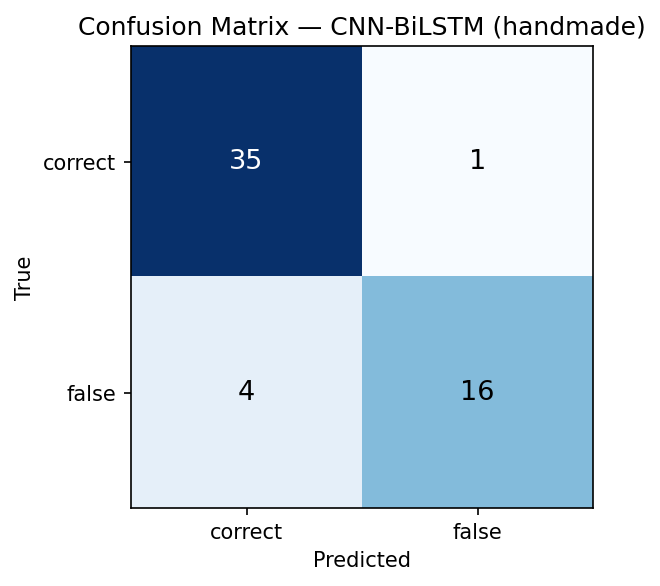
\includegraphics[width=0.60\textwidth]{figures/handmade_confusion_matrix.png}
\caption{Confusion matrix of the best handmade upper-bound model on the test set.}
\label{fig:cm-handmade}
\end{figure}
}{
\noindent\textit{Supplementary figure not available in the LaTeX tree:
\texttt{figures/handmade\_confusion\_matrix.png}.}
}

\IfFileExists{figures/autocorr_confusion_matrix.png}{
\begin{figure}[htbp]
\centering
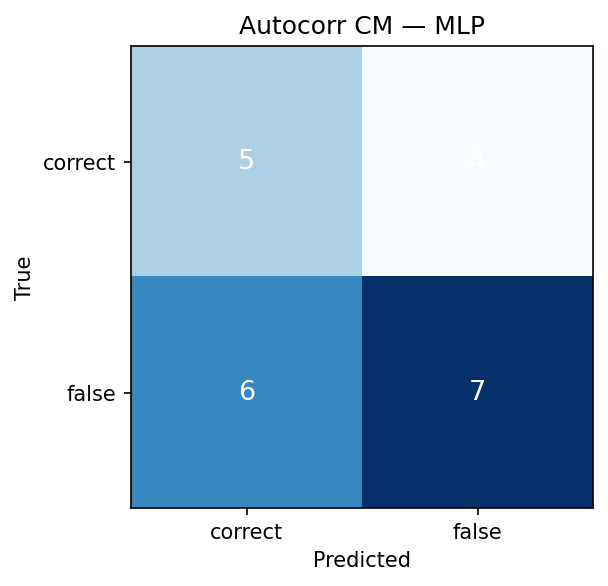
\includegraphics[width=0.60\textwidth]{figures/autocorr_confusion_matrix.png}
\caption{Confusion matrix of the autocorr landmark baseline on the test set.}
\label{fig:cm-autocorr}
\end{figure}
}{
\noindent\textit{Supplementary figure not available in the LaTeX tree:
\texttt{figures/autocorr\_confusion\_matrix.png}.}
}

\IfFileExists{figures/image_confusion_matrix.png}{
\begin{figure}[htbp]
\centering
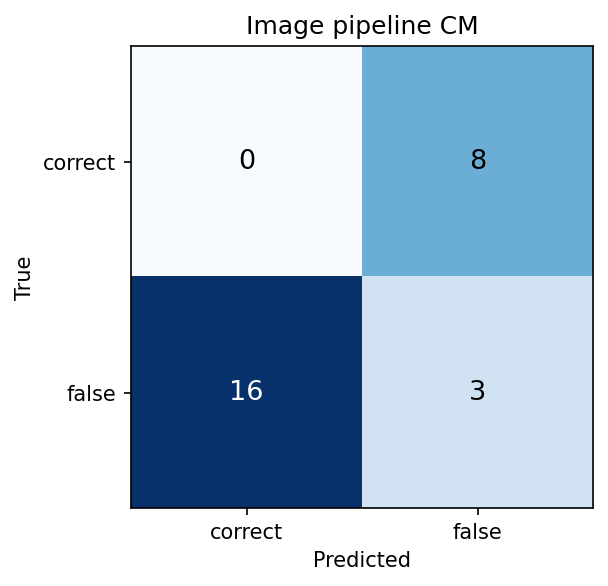
\includegraphics[width=0.60\textwidth]{figures/image_confusion_matrix.png}
\caption{Confusion matrix of the autocorr image-based pipeline on the test set.}
\label{fig:cm-image}
\end{figure}
}{
\noindent\textit{Supplementary figure not available in the LaTeX tree:
\texttt{figures/image\_confusion\_matrix.png}.}
}

% ---------------------------------------------------------------------
\section{Additional Signal Examples}
\label{app:signal-examples}

\IfFileExists{figures/contact_diff_signal_example.png}{
\begin{figure}[htbp]
\centering
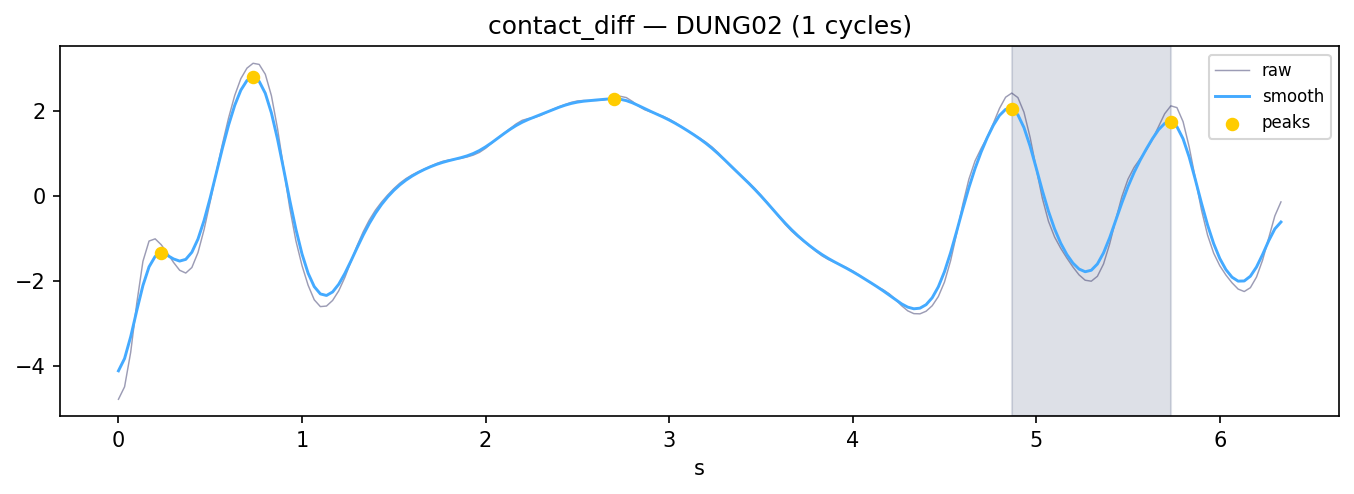
\includegraphics[width=0.80\textwidth]{figures/contact_diff_signal_example.png}
\caption{Example \texttt{contact\_diff} motion signal used for autocorrelation-based cycle detection.}
\label{fig:signal-contactdiff}
\end{figure}
}{
\noindent\textit{Supplementary figure not available in the LaTeX tree:
\texttt{figures/contact\_diff\_signal\_example.png}.}
}

\IfFileExists{figures/detected_cycle_example.png}{
\begin{figure}[htbp]
\centering
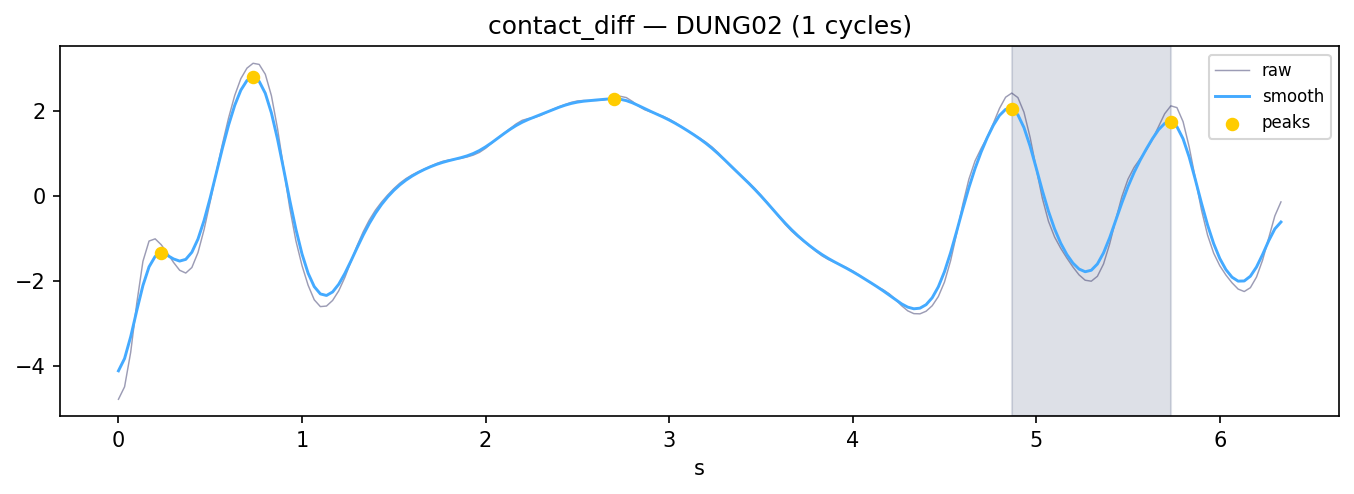
\includegraphics[width=0.80\textwidth]{figures/detected_cycle_example.png}
\caption{Example of an automatically detected foot-strike-to-foot-strike running cycle.}
\label{fig:detected-cycle}
\end{figure}
}{
\noindent\textit{Supplementary figure not available in the LaTeX tree:
\texttt{figures/detected\_cycle\_example.png}.}
}

\IfFileExists{figures/8phase_autocorr_sample.png}{
\begin{figure}[htbp]
\centering
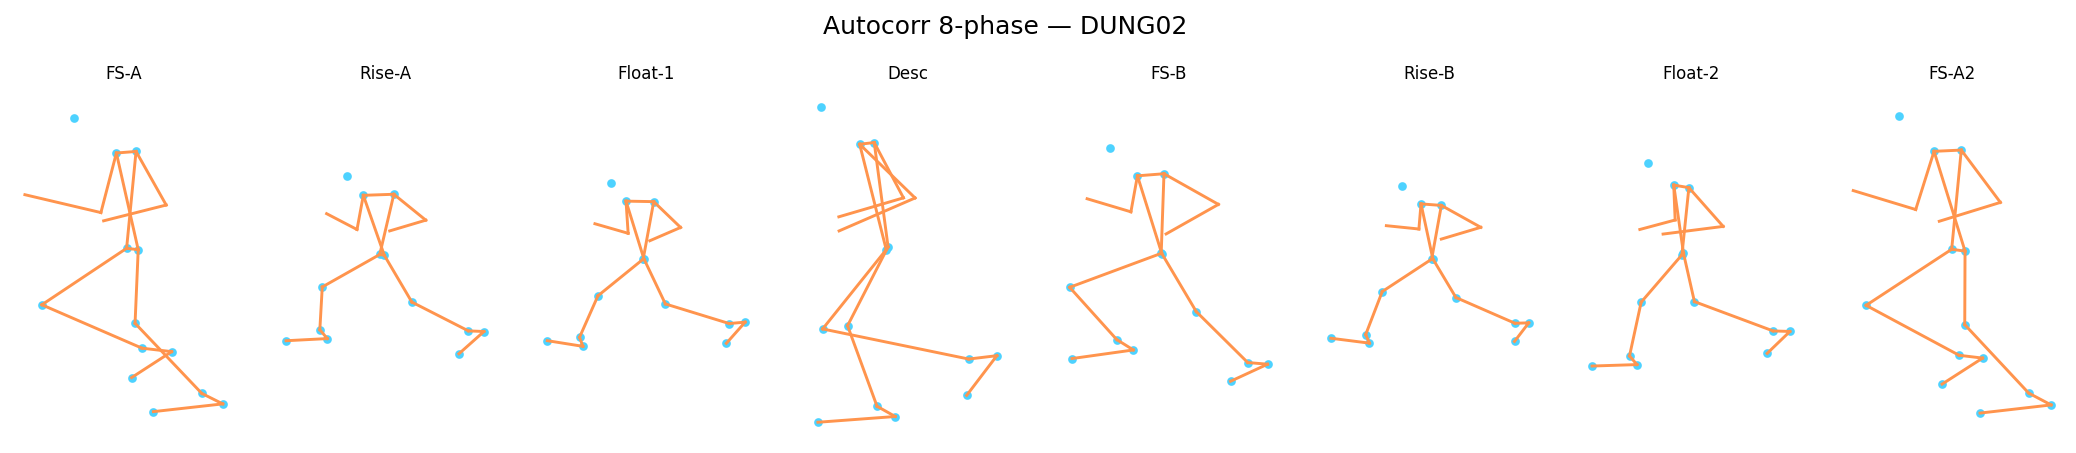
\includegraphics[width=0.80\textwidth]{figures/8phase_autocorr_sample.png}
\caption{Example eight-phase sampling of an automatically detected cycle.}
\label{fig:8phase-autocorr-sample}
\end{figure}
}{
\noindent\textit{Supplementary figure not available in the LaTeX tree:
\texttt{figures/8phase\_autocorr\_sample.png}.}
}

\IfFileExists{figures/period_distribution.png}{
\begin{figure}[htbp]
\centering
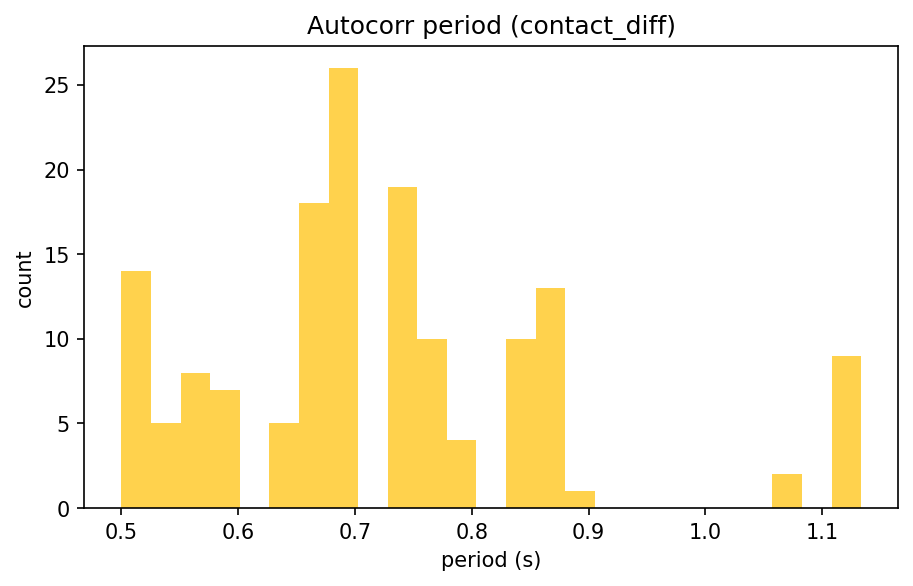
\includegraphics[width=0.70\textwidth]{figures/period_distribution.png}
\caption{Distribution of estimated cycle periods across detected videos.}
\label{fig:period-dist}
\end{figure}
}{
\noindent\textit{Supplementary figure not available in the LaTeX tree:
\texttt{figures/period\_distribution.png}.}
}

% ---------------------------------------------------------------------
\section{Training Curves}
\label{app:training-curves}

\IfFileExists{figures/handmade_training_curve.png}{
\begin{figure}[htbp]
\centering
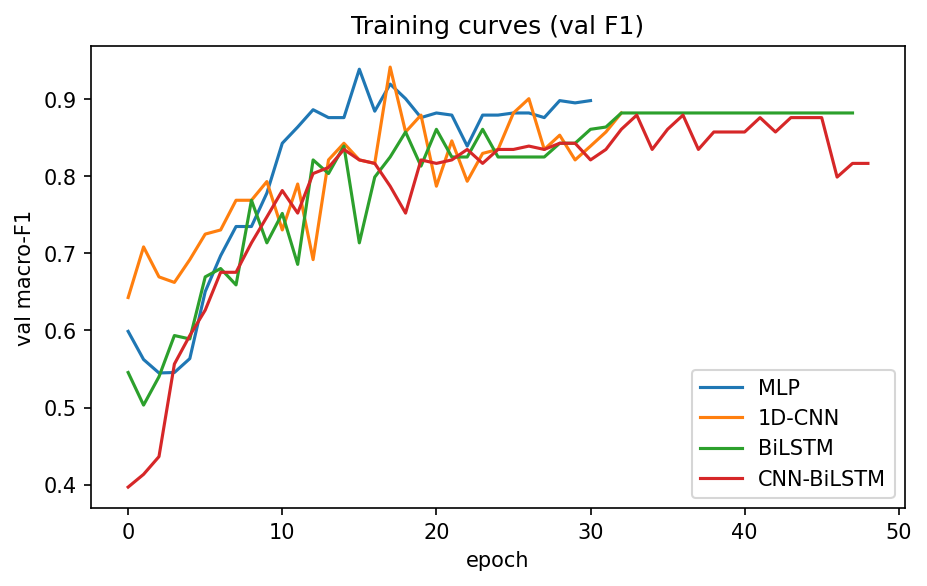
\includegraphics[width=0.80\textwidth]{figures/handmade_training_curve.png}
\caption{Training and validation curves for the handmade upper-bound models.}
\label{fig:curve-handmade}
\end{figure}
}{
\noindent\textit{Supplementary figure not available in the LaTeX tree:
\texttt{figures/handmade\_training\_curve.png}.}
}

\IfFileExists{figures/image_training_curve.png}{
\begin{figure}[htbp]
\centering
\includegraphics[width=0.80\textwidth]{figures/image_training_curve.png}
\caption{Training and validation curves for the autocorr image-based pipeline.}
\label{fig:curve-image}
\end{figure}
}{
\noindent\textit{Supplementary figure not available in the LaTeX tree:
\texttt{figures/image\_training\_curve.png}.}
}

% ---------------------------------------------------------------------
\section{Failed Case Examples}
\label{app:failed-cases}

\IfFileExists{figures/reject_reason_chart.png}{
\begin{figure}[htbp]
\centering
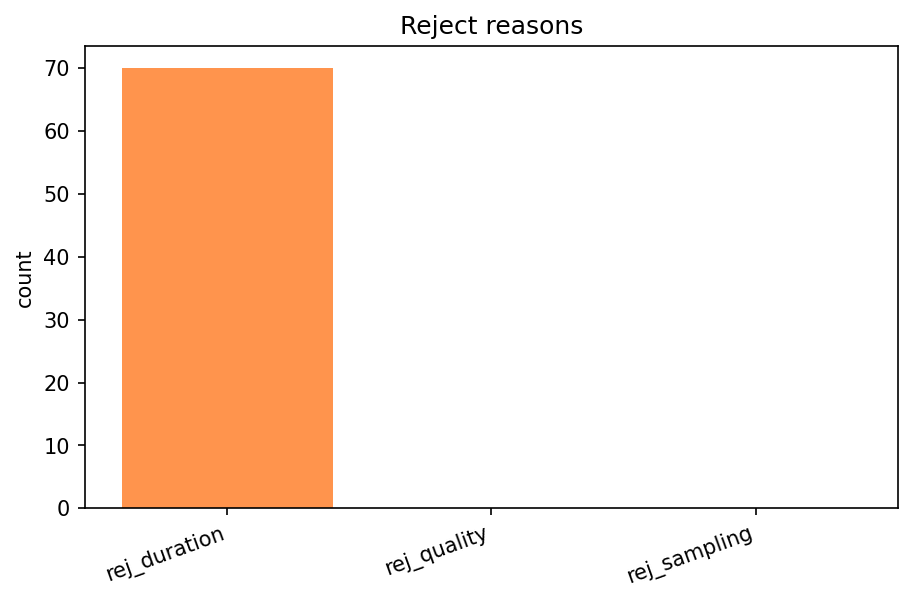
\includegraphics[width=0.70\textwidth]{figures/reject_reason_chart.png}
\caption{Breakdown of cycle-level rejection reasons in the autocorr pipeline.}
\label{fig:reject-reasons}
\end{figure}
}{
\noindent\textit{Supplementary figure not available in the LaTeX tree:
\texttt{figures/reject\_reason\_chart.png}.}
}

The per-video failure records are available in \path{outputs/autocorr/autocorr_failed_videos.csv} and the image-pipeline counterpart \path{outputs/autocorr_image/failed_videos.csv}, when those files are exported by the corresponding notebooks.


% ---------------------------------------------------------------------
\section{Fair Gap Robustness and Permutation Test}
\label{app:fair-gap}

Table~\ref{tab:app-fair-gap} records the supplementary robustness check used in
Section~\ref{sec:fair-gap}. It repeats the handmade--autocorr comparison with
the same MLP classifier, a fixed threshold of $0.5$, and 5-fold video-level
cross-validation. The values support the fixed-split conclusion that automatic
cycle detection is the main bottleneck.

\begin{table}[htbp]
\centering
\caption{Fair-gap robustness check and autocorr MLP permutation test. Source: \texttt{outputs/autocorr/fair\_gap\_and\_mlp\_perm.json}.}
\label{tab:app-fair-gap}
\renewcommand{\arraystretch}{1.18}
\scriptsize
\begin{tabularx}{\textwidth}{X r}
\toprule
\textbf{Quantity} & \textbf{Value} \\
\midrule
Handmade cycles / videos & 370 / 369 \\
Autocorr cycles / videos & 151 / 55 \\
Handmade 5-fold CV macro-F1 & $0.8597 \pm 0.0160$ \\
Handmade OOF macro-F1, 95\% CI & 0.8599 [0.8219, 0.8969] \\
Autocorr 5-fold CV macro-F1 & $0.6146 \pm 0.0809$ \\
Autocorr OOF macro-F1, 95\% CI & 0.6553 [0.5797, 0.7281] \\
Fair gap (handmade $-$ autocorr) & 0.2451 \\
Observed autocorr MLP CV macro-F1 in permutation test & 0.5206 \\
Permutation null mean $\pm$ std. & $0.4680 \pm 0.0740$ \\
Number of permutations & 100 \\
Permutation $p$-value & 0.2475 \\
\bottomrule
\end{tabularx}
\end{table}

The permutation result is interpreted conservatively. It does not prove that the
autocorr cycles contain no signal; it indicates that the signal is not robustly
separable under the tested simple MLP configuration and current sample size.


% ---------------------------------------------------------------------
\section{Autocorr Version History}
\label{app:version-history}

This section reproduces the autocorrelation version history for completeness.
\textbf{These are historical development results, not controlled benchmarks.}
The reported validation accuracies were recorded in development notebooks under
varying protocols and are \emph{not} directly comparable to the controlled
test metrics of Chapter~\ref{ch:results}. In particular,
\texttt{autocorr\_fixed(val\_acc 76.5)} is a historical image-based milestone
that motivated the organised image-based rerun. It must not be used to claim
that image-based modelling outperforms the landmark baseline unless rerun under
the same fixed-split protocol.

\begin{table}[htbp]
\centering
\caption{Autocorr version history. These rows describe historical development stages, not controlled benchmark results. Validation accuracies are reported only when they were recorded in development evidence.}
\label{tab:app-version-history}
\renewcommand{\arraystretch}{1.18}
\scriptsize
\begin{tblr}{
  % Trả colspec về dạng X chuẩn, cực kỳ an toàn cho hệ thống
  colspec = {X[1.3,l,m] X[1,l,m] X[1,l,m] X[1.6,l,m] Q[c,m]},
  rowsep = {4pt}, 
  hline{1,Z} = {0.08em}, 
  hline{2} = {0.05em},   
}
\textbf{Version} & \textbf{Signal} & \textbf{Input} & \textbf{Model} & \textbf{Val. acc.} \\

% Dùng \seqsplit{\texttt{...}} để ép chuỗi tự ngắt dòng khi chạm vách ngăn của cột
\seqsplit{\texttt{autocorr\_fixed\_val\_acc\_69\_6}} & head-Y oscillation & landmarks & CNN+LSTM / historical & 69.6\% \\

\seqsplit{\texttt{autocorr\_fixed\_val\_acc\_72\_9}} & \texttt{contact\_diff} & landmarks & CNN+LSTM / historical & 72.9\% \\

\seqsplit{\texttt{autocorr\_fixed\_biLSTM}} & \texttt{contact\_diff} & landmarks + velocity & BiLSTM & Not recorded \\

\seqsplit{\texttt{autocorr\_fixed\_val\_acc\_76\_5}} & \texttt{contact\_diff} + autocorr period & RGB crop $224 \times 224$ & MobileNetV2 + LSTM & 76.5\% \\

\end{tblr}
\end{table}

\noindent\textit{Note.} The historical validation values in
Table~\ref{tab:app-version-history} are development-stage records and are not
directly comparable to the fixed-split test metrics reported in
Chapter~\ref{ch:results}.

% ---------------------------------------------------------------------
\section{Historical Image-Based Autocorr Pipeline}
\label{app:historical-image-autocorr}

Among the historical autocorrelation-based experiments,
\texttt{autocorr\_fixed(val\_acc 76.5)} represents the most technically complex
development stage. Earlier autocorr versions mainly relied on pose-landmark
sequences and hand-crafted motion signals, such as head vertical oscillation or
contact-related landmark differences. In contrast, this version extended the
pipeline from landmark-based time-series classification to image-based sequence
modelling.

The pipeline first used markerless pose estimation to localise the runner and
extract foot-contact-related motion signals. The \texttt{contact\_diff} signal,
together with autocorrelation-based period estimation, was used to identify
running cycles. Instead of using only normalised landmark coordinates as the
input representation, each detected cycle was converted into an eight-phase RGB
image sequence. For each sampled phase, a runner-centred crop was generated
using a pose-derived bounding box, resized to a fixed image resolution, and
processed by a MobileNetV2-based visual feature extractor. A temporal LSTM head
then aggregated the eight-frame image sequence to classify the running
technique as correct or false.

This experiment is important because it tested whether visual appearance cues
that are absent from sparse landmark representations could improve
classification. RGB crops may preserve information about body silhouette, limb
contours, clothing-relative motion, and visual context that is lost when the
input is reduced to pose coordinates. Therefore, this notebook should be
described as a methodological extension from pose-only sequence classification
toward image-based running-cycle classification.

However, \texttt{autocorr\_fixed(val\_acc 76.5)} should not be used as the main
benchmark result. The reported 76.5\% value is a historical validation accuracy
from a development notebook and was not confirmed under the final fixed-split
evaluation and unified reporting protocol. For this reason, it is interpreted
as development evidence rather than final comparative evidence. The organised
image-based rerun is reported separately in Chapter~\ref{ch:results} as an
extended representation comparison.

% End of Appendix B


% -------------------- Bibliography --------------------
\clearpage
\printbibliography[heading=bibintoc] % Thêm danh mục tài liệu tham khảo vào Table of Contents

\end{document}